
%
% introduction.tex
% Copyright (C) 1995 by John Heidemann, <johnh@isi.edu>.
% $Id: demo2intr.tex,v 1.1 1996/01/12 18:13:58 johnh Exp $
%

\chapter{Non-tracial transport}\label{non-tracial transport chapter}

%%%%%%%%%%%%%%%%%%%%%%%%
%                 		Preliminaries	          		          %
%%%%%%%%%%%%%%%%%%%%%%%%

\section{Preliminaries}\label{prelim}



%	The free Araki-Woods factor and $q$-deformed Araki-Woods algebras
%%%%%%%%%%%%%%%%%%%%%%%%%%%%%%%%%%%%%%%%%%%%%
\subsection{The free Araki-Woods factor and $q$-deformed Araki-Woods algebras}\label{free_Araki-Woods}

Let $\H_\R$ be a real Hilbert space and $U_t$ a strongly continuous one-parameter group of orthogonal transformations on $\H_\R$. Letting $\H_\C:=\H_\R +\i \H_\R$ be the complexified Hilbert space, the $U_t$ can be extended to a one-parameter unitary group (still denoted as $U_t$). Let $A$ be the generator of the $U_t$ (i.e. $U_t=A^{it}$ and $A$ is a potentially unbounded positive operator). Let $\<\cdot,\cdot\>$ be the inner product on $\H_\C$ which is complex-linear in the second coordinate (as all other inner products will be in this section). Define an inner product $\<\cdot,\cdot\>_U$ on $\H_\C$ by
	\begin{align*}
		\<x,y\>_U  = \< \frac{2}{1+A^{-1}}x, y\>,\qquad x,y\in\H_\C.
	\end{align*}
Let $\H$ be the complex Hilbert space obtained by completing $\H_\C$ with respect to $\<\cdot,\cdot\>_U$. Note that if we start with the trivial one-parameter group $U_t=1$ for all $t$ then $A=1$, $\<\cdot,\cdot\>_U=\<\cdot,\cdot\>$ and $\H=\H_\C$. In this case we will write $\<\cdot,\cdot\>_1$ for $\<\cdot,\cdot\>_U$.\par
For $-1<q<1$, the $q$-Fock space $\mathcal{F}_q(\H)$ is the completion of $\mathcal{F}^{\text{finite}}(\H):=\bigoplus_{n=0}^\infty \H^{\otimes n}$, where $\H^{\otimes 0}=\C\Omega$ with vacuum vector $\Omega$, with respect to the sesquilinear form $\<\cdot,\cdot\>_{U,q}$ given by
	\begin{align*}
		\<f_1\otimes\cdots\otimes f_n, g_1\otimes\cdot\otimes g_m\>_{U,q} = \delta_{n=m} \sum_{\pi\in S_n} q^{i(\pi)} \<f_1,g_{\pi(1)}\>_U\cdots \<f_n,g_{\pi(n)}\>_U,
	\end{align*}
where $i(\pi)$ denotes the number of inversions of the permutation $\pi\in S_n$. We may at times denote $\mathcal{F}_q(\H_\R,U_t)=\mathcal{F}_q(\H)$ to emphasize $\{U_t\}$.

For any $h\in \H$ we can define the left $q$-creation operator $l(h)\in \B(\mc{F}_q(\H))$ by
	\begin{align*}
		&l_q(h)\Omega=h;\\
		&l_q(h)(f_1\otimes\cdots\otimes f_n)=h\otimes f_1\otimes\cdots \otimes f_n,
	\end{align*}
then its adjoint is the left $q$-annihilation operator:
	\begin{align*}
		&l_q^*(h)\Omega=0;\\
		&l_q^*(h)(f_1\otimes\cdots\otimes f_n)= \sum_{i=1}^n q^{i-1} \<h,f_i\>_U f_1\otimes \cdots \otimes f_{i-1}\otimes f_{i+1}\otimes\cdots \otimes f_n.
	\end{align*}
Also define
	\begin{align*}
		s_q(h):=l_q(h)+l_q^*(h).
	\end{align*}\par
We let $\Gamma_q(\H_\R,U_t)$ be the $C^*$-algebra generated by $\{s_q(h)\colon h\in\H_\R\}$. The corresponding von Neumann algebra $M_q:=\Gamma_q(\H_\R,U_t)''\subset \B(\mc{F}_q(\H))$ is called a \emph{$q$-deformed Araki-Woods algebra}, after \cite{Hia03}, except when $q=0$ where $M_0=\Gamma_0(\H_\R,U_t)''$ is called a \emph{free Araki-Woods factor}, after \cite{Shl97}.\par
It was shown in \cite{Hia03} that $\Omega$ is a cyclic and separating vector for $M_q$ and consequently the vacuum state $\varphi_q(\cdot)=\<\Omega,\cdot\  \Omega\>_{U,q}$ is faithful. For $q\neq 0$, $\varphi_q$ is called the \emph{$q$-quasi-free state}, or the \emph{$q$-quasi-free state associated to $A$}. For $q=0$, $\varphi_0$ is called the \emph{free quasi-free state}, or the \emph{free quasi-free state associated to $A$}.\par

\begin{rem}
For $f_1,\ldots, f_n\in \H_\R$, computing $\varphi_q(s_q(f_1)\cdots s_q(f_n))$ is best done diagrammatically through non-crossing (when $q=0$) and crossing (when $q\neq 0$) pairing diagrams. When $q=0$, visualize a rectangle with the vectors $f_1,\ldots, f_n$ arranged in order along the top:
	\begin{equation*}
		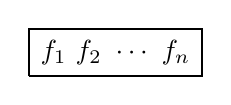
\begin{tikzpicture}
			\draw [thick] (0,0) -- (0,0.6) -- (2.2,0.6) -- (2.2,0) -- (0,0);
			\node at (1.1,0.3) {$f_1\ f_2\ \cdots\ f_n$};
		\end{tikzpicture}.
	\end{equation*}
$\varphi(s(f_1)\cdots s(f_n))$ counts all the ways to pair the vectors to each other via chords above the rectangle so that no two chords intersect and if a vector $f_i$ is connected to a vector $f_j$ (with $f_i$ on the left) then that diagram is weighted by a factor of $\<f_i,f_j\>_U$. For example the following diagram has the denoted weight:
	\begin{equation*}
		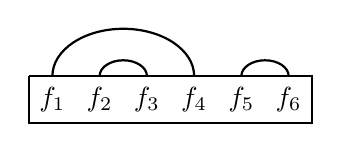
\begin{tikzpicture}[baseline]
			\draw [thick] (0,0.3) -- (0,-0.3) -- (3.6,-0.3) -- (3.6,0.3) -- (0,0.3);
			\node at (.3,0) {$f_1$};
			\node at (.9,0) {$f_2$};
			\node at (1.5,0) {$f_3$};
			\node at (2.1,0) {$f_4$};
			\node at (2.7,0) {$f_5$};
			\node at (3.3,0) {$f_6$};
			\draw[thick] (2.1,0.3) arc (0:180:0.9 and 0.6); %coordinate marks the right end-point of the semi-circle NOT the center
			\draw[thick] (1.5,0.3) arc (0:180:0.3 and 0.2);
			\draw[thick] (3.3,0.3) arc (0:180:0.3 and 0.2);
		\end{tikzpicture}
		=\<f_1,f_4\>_U\<f_2,f_3\>_U\<f_5,f_6\>_U.
	\end{equation*}
Thus
	\begin{align*}
		\varphi(s(f_1)s(f_2)s(f_3)s(f_4)) &= 
			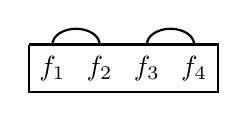
\begin{tikzpicture}[baseline]
			\draw [thick] (0,0.3) -- (0,-0.3) -- (2.4,-0.3) -- (2.4,0.3) -- (0,0.3);
			\node at (.3,0) {$f_1$};
			\node at (.9,0) {$f_2$};
			\node at (1.5,0) {$f_3$};
			\node at (2.1,0) {$f_4$};
			\draw[thick] (0.9,0.3) arc (0:180:0.3 and 0.2);
			\draw[thick] (2.1,0.3) arc (0:180:0.3 and 0.2);
			\end{tikzpicture}
		+
			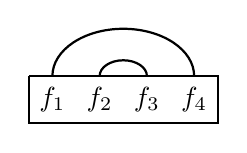
\begin{tikzpicture}[baseline]
			\draw [thick] (0,0.3) -- (0,-0.3) -- (2.4,-0.3) -- (2.4,0.3) -- (0,0.3);
			\node at (.3,0) {$f_1$};
			\node at (.9,0) {$f_2$};
			\node at (1.5,0) {$f_3$};
			\node at (2.1,0) {$f_4$};
			\draw[thick] (2.1,0.3) arc (0:180:0.9 and 0.6);
			\draw[thick] (1.5,0.3) arc (0:180:0.3 and 0.2);
			\end{tikzpicture}\\
		&=\<f_1,f_2\>_U\<f_3,f_4\>_U + \<f_1, f_4\>_U\<f_2,f_3\>_U.
	\end{align*}
Note that $\varphi$ then clearly takes a value of zero on all monomials of odd degree.\par
When $q\neq 0$, the chords may intersect and do so at the cost of a factor of $q$ for each intersection. Revisiting the previous example in this case we then have
	\begin{align*}
		\varphi_q(s_q(f_1)s_q(f_2)s_q(f_3)s_q(f_4)) &= 
			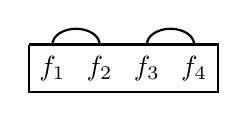
\begin{tikzpicture}[baseline]
			\draw [thick] (0,0.3) -- (0,-0.3) -- (2.4,-0.3) -- (2.4,0.3) -- (0,0.3);
			\node at (.3,0) {$f_1$};
			\node at (.9,0) {$f_2$};
			\node at (1.5,0) {$f_3$};
			\node at (2.1,0) {$f_4$};
			\draw[thick] (0.9,0.3) arc (0:180:0.3 and 0.2);
			\draw[thick] (2.1,0.3) arc (0:180:0.3 and 0.2);
			\end{tikzpicture}
		+
			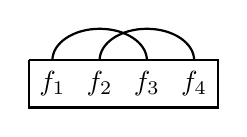
\begin{tikzpicture}[baseline]
			\draw [thick] (0,0.3) -- (0,-0.3) -- (2.4,-0.3) -- (2.4,0.3) -- (0,0.3);
			\node at (.3,0) {$f_1$};
			\node at (.9,0) {$f_2$};
			\node at (1.5,0) {$f_3$};
			\node at (2.1,0) {$f_4$};
			\draw[thick] (1.5,0.3) arc (0:180:0.6 and 0.4);
			\draw[thick] (2.1,0.3) arc (0:180:0.6 and 0.4);
			\end{tikzpicture}
		+
			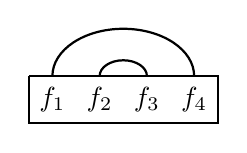
\begin{tikzpicture}[baseline]
			\draw [thick] (0,0.3) -- (0,-0.3) -- (2.4,-0.3) -- (2.4,0.3) -- (0,0.3);
			\node at (.3,0) {$f_1$};
			\node at (.9,0) {$f_2$};
			\node at (1.5,0) {$f_3$};
			\node at (2.1,0) {$f_4$};
			\draw[thick] (2.1,0.3) arc (0:180:0.9 and 0.6);
			\draw[thick] (1.5,0.3) arc (0:180:0.3 and 0.2);
			\end{tikzpicture}\\
		&=\<f_1,f_2\>_U\<f_3,f_4\>_U + q\<f_1,f_3\>_U\<f_2,f_4\>_U + \<f_1, f_4\>_U\<f_2,f_3\>_U.
	\end{align*}
We note that in computing $\varphi_q(s_q(f_1)s_q(f_2)s_q(f_3)s_q(f_4))=\<\Omega, s_q(f_1)s_q(f_2)s_q(f_3)s_q(f_4)\Omega\>_{U,q}$ by writing out $s_q(f_1)s_q(f_2)s_q(f_3)s_q(f_4)\Omega$, the term $ q\<f_1,f_3\>_U\<f_2,f_4\>_U$ comes from when $s_q(f_1)s_q(f_2)$ acts on $f_3\otimes f_4$ and the operator $l_q^*(f_2)$ ``skips'' over the the first vector in the tensor product (hence the factor of $q$).\par
It is a worthwhile exercise to restrict to the case when there is only a single operator $s_q(f)$ (so that all inner-products are $1$) and draw out the diagrams corresponding to $\varphi(s_q(f)^n)$ for $n=2,4,6,8$.
\end{rem}

The Tomita-Takesaki theory for $M_q$ is established in Lemma 1.4 of \cite{Hia03}, which we recall here for convenience. Let $S$ denote the closure of the map $x\Omega\mapsto x^*\Omega$, and let $S=J\Delta^{1/2}$ be its polar decomposition so that $J$ and $\Delta$ are the modular conjugation and modular operator, respectively. Then for $n\geq 1$
	\begin{align}\label{Tomita-Takesaki_formulas}
		S(f_1\otimes\cdots\otimes f_n)&=f_n\otimes \cdots \otimes f_n	&\text{for }f_1,\ldots, f_n\in\H_\R;\notag\\
		\Delta(f_1\otimes\cdots\otimes f_n)&=(A^{-1}f_1)\otimes \cdots\otimes (A^{-1} f_n)		&\text{for }f_1,\ldots,f_n\in \H_\R\cap \text{dom}{A^{-1}};\\
		J(f_1\otimes\cdots\otimes f_n)&=(A^{-1/2} f_n)\otimes\cdots \otimes (A^{-1/2}f_n)		&\text{for }f_1,\ldots, f_n\in \H_\R\cap\text{dom}{A^{-1/2}}.\notag
	\end{align}
Denote by $\sigma_t^{\varphi_q}(\cdot)= \Delta^{it} \cdot \Delta^{-it}$ the modular automorphism group of $\varphi_q$.\par
Henceforth we assume $\dim(\H_\R)=N<\infty$. Consequently $A$ and $A^{-1}$ are bounded operators and hence $\{\sigma_t^{\varphi_q}\}_{t\in\R}$ extends to $\{\sigma_z^{\varphi_q}\}_{z\in\C}$. In particular for $a,b\in M$,
	\begin{align*}
		\varphi(ab)&=\< a^*\Omega, b\Omega\>_{U,q}=\< S a\Omega, b\Omega\>_{U,q}=\<Jb\Omega, \Delta^\frac{1}{2} a\Omega\>_{U,q}\\
				&=\< \Delta \Delta^{-\frac{1}{2}} Jb\Omega,a\Omega\>_{U,q} = \< \Delta b^*\Omega, a\Omega\>_{U,q}= \varphi(\sigma_{i}^{\varphi_q}(b) a).
	\end{align*}
Moreover, the action of $\Delta$ in (\ref{Tomita-Takesaki_formulas}) extends to $f_1,\ldots, f_n\in \H$.\par
From Remark 2.12 in \cite{Shl97} it follows that for a suitable orthonormal basis $\{e_1,\ldots,e_N\}$ of $(\H_\R,\<\cdot,\cdot\>)$, the generator $A$ can be represented as a matrix of the form
	\begin{equation}\label{matrix_form_A}
		A=\text{diag}\left( A_1,\ldots, A_L,1,\ldots,1\right),
	\end{equation}
where for each $k\in\{1,\ldots,L\}$
	\begin{equation}\label{matrix_form_A_2}
		A_k=\frac{1}{2}\left(\begin{array}{cc}
						\lambda_k+\lambda_k^{-1}		& -i\left(\lambda_k-\lambda_k^{-1}\right)	\\
						i\left(\lambda_k-\lambda_k^{-1}\right)	& \lambda_k+\lambda_k^{-1}	\end{array}\right)\in M_2(\C),
	\end{equation}
and $\lambda_k>0$. Note that
	\begin{equation*}
		A_k^{it}=\left(\begin{array}{cc}	\cos(t\log{\lambda_k})	&	-\sin(t\log{\lambda_k})\\
								\sin(t\log{\lambda_k}) 	& 	\cos(t\log{\lambda_k})\end{array}\right),
	\end{equation*}
which is a unitary matrix such that $(A_k^{it})^*=(A_k^{it})^\text{T}=A_k^{-it}$. $A$ has the following properties:
	\begin{enumerate}
		\item[1.] $\text{spectrum}(A)=\left\{1,\lambda_1^{\pm 1},\ldots, \lambda_L^{\pm 1}\right\}$;
		\item[2.] $A^\text{T}=A^{-1}$;
		\item[3.] $\left( A^{it}\right)^*=\left( A^{it}\right)^\text{T}=A^{-it}$; and
		\item[4.] for any fixed $i\in\{1,\ldots, N\}$, 
			\begin{equation*}
				\sum_{j=1}^N \left|[A]_{ij}\right|\leq \max\left\{1,\lambda_1^{\pm 1},\ldots, \lambda_L^{\pm 1}\right\}\leq \|A\|.
			\end{equation*}
	\end{enumerate}
For each $j=1,\ldots, N$, let $X_j^{(q)}=s_q(e_j)$ and write $X^{(q)}=(X_1^{(q)},\ldots, X_N^{(q)})$. Since $s_q$ is real linear, it follows that $M_q=W^*(X_1^{(q)},\ldots, X_N^{(q)})$. We observe that
	\begin{align*}
		\sigma_z^{\varphi_q}(X_j^{(q)})=\sum_{k=1}^N [A^{iz}]_{jk} X_k^{(q)},\qquad \forall z\in \C,
	\end{align*}
or using the vector notation:
	\begin{align}\label{modular_semicircular}
		\sigma_z^{\varphi_q}(X^{(q)})= A^{iz} X^{(q)},\qquad \forall z\in\C.
	\end{align}
Indeed, using (\ref{Tomita-Takesaki_formulas}) it is easy to see that
	\begin{align*}
		\sigma_z^{\varphi_q}(l_q(e_j))&= l_q(A^{-iz} e_j)\\
		\sigma_z^{\varphi_q}(l_q^*(e_j))&=l_q^*( A^{-i\bar{z}} e_j).
	\end{align*}
Equation (\ref{modular_semicircular}) follows from the above properties of $A$, the linearity of $l_q$, and the conjugate linearity of $l_q^*$.


%	Derviations on $M_q$
%%%%%%%%%%%%%%%%%%%%%%%%%%%%%%%%%%%%%%%%
\subsection{Derivations on $M_q$}\label{derivations_on_M_q}

For the remainder of this section we will consider a single fixed $q\in (-1,1)$, so that we may repress the superscript $(q)$ notation on $X^{(q)}_j$, and write $\mathscr{P}$ for the $*$-subalgebra $\C\<X_1,\ldots, X_N\>\subset M_q$ of non-commutative polynomials in $N$-variables. We also simplify notation with $M:=M_q$, $\varphi:=\varphi_q$, and $\sigma_z:=\sigma_z^{\varphi_q}$ for $z\in \C$.\par
For each $j\in\{1,\ldots,N\}$ we let $\delta_j\colon \mathscr{P}\rightarrow \mathscr{P}\otimes\mathscr{P}^{op}$ be Voiculescu's free-difference quotient:
	\begin{align*}
		\delta_j(X_{i_1}\cdots X_{i_n})=\sum_{k=1}^n \delta_{j=i_k} X_{i_1}\cdots X_{i_{k-1}}\otimes \left(X_{i_{k+1}}\cdots X_{i_n}\right)^\circ;
	\end{align*}
that is, $\delta_j$ is the unique derivation satisfying $\delta_j(X_i)=\delta_{j=i}1\otimes 1$. We set the following conventions for working with elementary tensors in $\mathscr{P}\otimes\mathscr{P}^{op}$:
	\begin{itemize}
		\item $(a\otimes b^\circ)\#(c\otimes d^\circ):= (ac)\otimes (b^\circ d^\circ)=(ac)\otimes (db)^\circ$;
		\item $(a\otimes b^\circ)\#c=acb$;
		\item $(a\otimes b^\circ)^*:=a^*\otimes (b^*)^\circ$;
		\item $(a\otimes b^\circ)^\dagger:= b^*\otimes (a^*)^\circ$;
		\item $(a\otimes b^\circ)^\diamond:= b\otimes a^\circ$;
		\item $m(a\otimes b^\circ):=ab$.
	\end{itemize}
We also define the left and right actions of $\mathscr{P}$ as:
	\begin{itemize}
		\item $c\cdot (a\otimes b^\circ):=(ca)\otimes b^\circ$;
		\item $(a\otimes b^\circ)\cdot c:=a\otimes (bc)^\circ$.
	\end{itemize}
Note that 
	\begin{align*}
		c\cdot (a\otimes b^\circ)&= (c\otimes 1^\circ)\# (a\otimes b^\circ),\ \text{and}\\
		(a\otimes b^\circ)\cdot c &= (1\otimes c^\circ )\# (a\otimes b^\circ).
	\end{align*}
We will usually suppress the notation ``$\circ$" and at times represent tensors  of monomials in $\mathscr{P}$ diagrammatically as follows:
	\begin{align}\label{box_notation}
	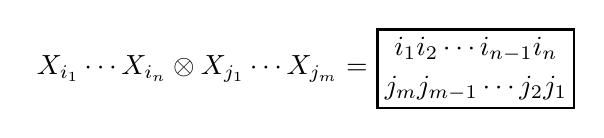
\begin{tikzpicture}[baseline]
	\draw[thick] (0,-.5) rectangle (2.5,.5);
	\node[left] at (0,0) {$X_{i_1}\cdots X_{i_n}\otimes X_{j_1}\cdots X_{j_m}=$};
	\node at (1.25,.25) {$i_1i_2\cdots i_{n-1}i_n$};
	\node at (1.25,-.25) {$j_mj_{m-1}\cdots j_2j_1$};
	\end{tikzpicture}.
	\end{align}
Then multiplication is neatly expressed as:
	\begin{align*}
	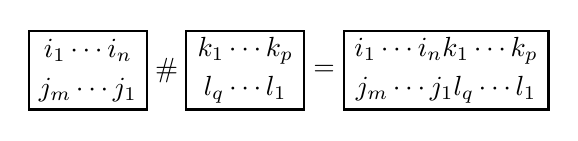
\begin{tikzpicture}[baseline]
	\draw[thick] (0,-.5) rectangle (1.5,.5);
	\node at (.75,.25) {$i_1\cdots i_n$};
	\node at (.75,-.25) {$j_m\cdots j_1$};
	\node at (1.75,0) {$\#$};
	\draw[thick] (2,-.5) rectangle (3.5,.5);
	\node at (2.75,.25) {$k_1\cdots k_p$};
	\node at (2.75,-.25) {$l_q\cdots l_1$};
	\node at (3.75,0) {$=$};
	\draw[thick] (4,-.5) rectangle (6.6,.5);
	\node at (5.3,.25) {$i_1\cdots i_nk_1\cdots k_p$};
	\node at (5.3,-.25) {$j_m\cdots j_1l_q\cdots l_1$};
	\end{tikzpicture}.
	\end{align*}
We note the involutions $*,\dagger,\diamond$ amount to horizontal reflection, vertical reflection, and $180^\circ$ rotation of the diagrams, respectively.\par
For $j,k\in\{1,\ldots, N\}$, we use the shorthand notation
	\begin{align*}
		\alpha_{jk}:=\left[ \frac{2}{1+A}\right]_{jk} =\<e_k,e_j\>_U.
	\end{align*}
Note that the last equality implies $\overline{\alpha_{jk}}=\alpha_{kj}$, $\alpha_{jj}=1$, and $|\alpha_{jk}|\leq 1$ for all $j,k\in\{1,\ldots, N\}$.\par
Let $\Xi_q \in HS(\mc{F}_q(\H))$ be the Hilbert-Schmidt operator on $\mc{F}_q(\H)$ given by the sum $\sum_{n=0}^\infty q^n P_n$ where $P_n\colon \mc{F}_q(\H) \rightarrow \H^{\otimes n}$ is the projection onto vectors of length $n$. We identify the Hilbert space generated by the GNS construction with respect to $\varphi\otimes\varphi^{op}$ with $L^2(M\bar{\otimes}M^{op},\varphi\otimes\varphi^{op})\cong HS(\mc{F}_q(\H))$ via $a\otimes b^\circ\mapsto \<\Omega, b\ \cdot\>a\Omega$ (\emph{cf.} Proposition 5.11 in \cite{Voi94}); in particular, $\Xi_0= P_0$ corresponds to $1\otimes 1$. Realize that the involution $\dagger$ defined above corresponds precisely with the adjoint operation in $HS(\mc{F}_q(\H))$. Consequently, $\Xi_q^\dagger=\Xi_q$ since, as a real sum of projections, it is a self-adjoint Hilbert-Schmidt operator.\par
For each $j=1,\ldots, N$ we define the derivation $\partial_j^{(q)}\colon\mathscr{P}\rightarrow \mathscr{P}\otimes \mathscr{P}^{op}$ by
	\begin{align*}
		\partial_j^{(q)}(P)=\sum_{k=1}^N \alpha_{kj}\delta(P)\#\Xi_q.
	\end{align*}
That is, $\partial_j^{(q)}$ is the unique derivation satisfying $\partial_j^{(q)}(X_i)=\alpha_{ij}\Xi_q$. We shall also consider the derivations
	\begin{align*}
		\bar{\partial}_j^{(q)}(P):=\sum_{k=1}^N \alpha_{jk}\delta_k(P)\# \Xi_q\qquad\text{ and }\qquad \tilde{\partial}_j^{(q)} :=\sum_{k=1}^N \alpha_{jk} \left(\delta_k(P)\# \Xi_q\right)^\diamond,
	\end{align*}
which are related to $\partial_j^{(q)}$ by
	\begin{align*}
		\partial_j^{(q)}(P)^\dagger=\bar{\partial}_j^{(q)}(P^*)\qquad\text{ and }\qquad \partial_j^{(q)}(P)^* = \tilde{\partial}_j^{(q)}(P^*).
	\end{align*}
We remark that in the tracial case ($U_t=1_t$), we have $\bar{\partial}_{j}^{(q)}=[\cdot, r_q(e_j)]$, where $r_q(e_j)$ is the right $q$-creation operator. This is precisely the derivation considered in Lemma 27 of \cite{D}.\par
From (\ref{modular_semicircular}) we see that
	\begin{align*}
		\partial_j^{(q)}(\sigma_{it}(X_k))=\sum_{l=1}^N [A^{-t}]_{kl} \alpha_{lj} \Xi_q = \left[\frac{2A^{-t}}{1+A}\right]_{kj} \Xi_q,
	\end{align*}
and thus $(\sigma_{-it}\otimes\sigma_{-it})\circ\partial_j\circ\sigma_{it}$ defines the unique derivation satisfying $X_k\mapsto \left[\frac{2A^{-t}}{1+A}\right]_{kj}\Xi_q$. In particular, since
	\begin{align*}
		\left[\frac{2A}{1+A}\right]_{kj}=\left[\frac{2}{1+A^{-1}}\right]_{kj}=\left[\frac{2}{1+A}\right]_{jk},
	\end{align*}
we see that
	\begin{equation}\label{differentiating_sigma_with_q}
		(\sigma_i\otimes\sigma_i)\circ\partial_j^{(q)}\circ\sigma_{-i}=\bar{\partial}_j^{(q)}.
	\end{equation}
The motivation for considering such derivations is precisely the following proposition.

\begin{prop}\label{adjoint_of_q-derivations}
View $\partial_j^{(q)}$ and $\bar{\partial}_j^{(q)}$ as densely defined operators from $L^2(\mathscr{P},\varphi)$ to $L^2(\mathscr{P}\otimes \mathscr{P}^{op},\varphi\otimes\varphi^{op})$. Then $1\otimes 1\in \dom{\partial_j^{(q)*}}$ with
	\begin{equation}\label{adjoint_of_1}
		\partial_j^{(q)*}(1\otimes 1)=X_j.
	\end{equation}
Moreover, $1\otimes1\in\dom{\bar{\partial}_j^{(q)*}}$ with
	\begin{equation}
		\bar{\partial}_j^{(q)*}(1\otimes 1)=\sigma_{-i}(X_j).
	\end{equation}
\end{prop}

\begin{rem}
The above proposition states that $X_1,\ldots, X_N$ (resp. $\sigma_{-i}(X_1),\ldots, \sigma_{-i}(X_N)$) are \emph{conjugate variables to $X$ with respect to the derivations $\partial_1^{(q)},\ldots, \partial_N^{(q)}$}  (resp. $\bar{\partial}_1^{(q)},\ldots, \bar{\partial}_N^{(q)}$) (\emph{cf.} Section 3 of \cite{Voi94}).
\end{rem}

\begin{proof}
Consider the monomial $P=X_{i_1}\cdots X_{i_n}\in\mathscr{P}$. Then,
	\begin{align*}
		\varphi(X_j P)=\<X_j\Omega, P\Omega\>_{U,q} = \< P_1X_j\Omega, P\Omega\>_{U,q} = \<P_1X_j\Omega, P_1P\Omega\>_{U,q},
	\end{align*}
where $P_1\in \B (\mc{F}_q(\H))$ is the projection onto tensors of length one. As $P$ is a product of the $X_{i_k}$, it is clear that $P_1P\Omega$ will be a linear combination of $e_{i_1},\ldots, e_{i_n}$, say $P_1P\Omega=\sum_{k=1}^n c_k e_{i_k}$. We claim that
	\begin{align*}
		c_k =\sum_{l=0}^\infty q^l \< P_l X_{i_{k-1}}\cdots X_{i_1}\Omega, P_l X_{i_{k+1}}\cdots X_{i_n}\Omega\>_{U,q}.
	\end{align*}
Indeed, diagrammatically each term contributing to $c_k$ is a pairing of the vectors $e_{i_1},\ldots, e_{i_n}$ with $e_{i_k}$ excluded. We can arrange such pairings according to the number of pairs whose connecting chords cross over $e_{i_k}$. Fix $l\geq 0$ and consider pairings with $l$ chords passing over $e_{i_k}$. Write $P=A_kX_{i_k}B_k$, then $P_lB_k\Omega$ gives pairings within $B_k$ that leave $l$ vectors unpaired. Hence $\<\Omega, A_kP_lB_k\Omega\>$ counts the pairings in which there are exactly $l$ pairs with one vector coming from $A_k$ and one coming from $B_k$. Since the cost of skipping over $e_{i_k}$ $l$ times is $q^l$ we see that
	\begin{equation*}
		c_k = \sum_{l=0}^\infty q^l \<\Omega, A_kP_l B_k\Omega\>_{U,q} = \sum_{l=0}^\infty q^l \< P_l A_k^*\Omega, P_l B_k\Omega\>_{U,q},
	\end{equation*}
as claimed. Thus
	\begin{align*}
		\< P_1X_j\Omega, P_1P\Omega\>_{U,q} =\sum_{k=1}^n \< P_1 X_j\Omega, e_{i_k}\>_{U,q} c_k = \sum_{k=1}^n \<e_j, e_{i_k}\>_U  \sum_{l=0}^\infty q^l \< P_l A_k^*\Omega, P_l B_k\Omega\>_{U,q}.
	\end{align*}\par
Now, we inductively orthonormalize the monomials $X_{\ul{i}}\in\mathscr{P}$ with respect to $\<\cdot\ \Omega,\cdot\ \Omega\>_{U,q}$ to obtain a basis $\{r_{\ul{j}}\}_{|\ul{j}|\geq 0}$ so that for each $l$, $\text{span}\{r_{\ul{j}}\colon |\ul{j}|=l\}=\text{span}\{X_{\ul{i}}\colon |\ul{i}|=l\}$. Then $P_lB_k=\sum_{|\ul{j}|=l} \<r_{\ul{j}}\Omega, B\Omega\>_{U,q} r_{\ul{j}}$ and using our identification with $L^2(M\bar{\otimes}M^{op},\varphi\otimes\varphi^{op})$ we see that $P_l = \sum_{|\ul{j}|=l} r_{\ul{j}}\otimes r_{\ul{j}}^*$. Thus we have
	\begin{align*}
		\varphi(X_jP) &= \sum_{k=1}^n \<e_j, e_{i_k}\>_{U}\sum_{l=0}^\infty q^l \< P_l A_k^*\Omega, P_l B_k\Omega\>_{U,q}\\
			&= \sum_{k=1}^n \< e_j, e_{i_k}\>_U \sum_{l=0}^\infty q^l \sum_{|\ul{j}|=l}\< A_k^*\Omega, r_{\ul{j}}\Omega\>_{U,q}\<r_{\ul{j}}\Omega, B_k\Omega\>_{U,q}\\
			&= \sum_{k=1}^n \<e_j, e_{i_k}\>_U \sum_{l=0}^\infty q^l \sum_{|\ul{j}|=l} \varphi\otimes\varphi^{op}\left( A_k\otimes B_k \# r_{\ul{j}}\otimes r_{\ul{j}}^* \right)\\
			&= \sum_{k=1}^n \<e_j, e_{i_k}\>_U \varphi\otimes \varphi^{op}\left( A_k\otimes B_k \#\Xi_q\right) \\
			&= \varphi\otimes \varphi^{op}\left( \partial_j^{(q)}P \right),
	\end{align*}
or $\<X_j, P\>_{\varphi} = \< 1\otimes 1, \partial_j^{(q)}P\>_{\varphi\otimes\varphi^{op}}$, which implies $\partial_j^{(q)*}(1\otimes 1)=X_j$.\par
Now,
	\begin{align*}
		\<\sigma_{-i}(X_j),P\>_{\varphi}&=\varphi(\sigma_i(X_j)P)=\varphi(PX_j)=\<P^*,\partial_j^{(q)*}(1\otimes 1)\>_{\varphi}=\<\bar{\partial}_j^{(q)}(P)^\dagger,1\otimes 1\>_{\varphi}\\
			&=\varphi\otimes\varphi^{op}( \bar{\partial}_j^{(q)}(P)^\diamond)=\varphi\otimes\varphi^{op}(\bar{\partial}_j^{(q)}(P))=\<1\otimes 1, \bar{\partial}_j^{(q)}(P)\>_{\varphi},
	\end{align*}
so that $1\otimes 1\in \text{dom}\left(\bar{\partial}_j^{(q)}\right)$ and $\bar{\partial}_j^{(q)*}(1\otimes 1)=\sigma_{-i}(X_j)$.
\end{proof}

\begin{cor}\label{difference_quotient_adjoint}
Viewing $\partial_j^{(q)}\colon L^2(\mathscr{P},\varphi)\rightarrow L^2(\mathscr{P}\otimes\mathscr{P}^{op},\varphi\otimes\varphi^{op})$ as a densely defined operator we have $\mathscr{P}\otimes\mathscr{P}^{op}\subset \dom{\partial_j^{(q)*}}$. In particular, if $\eta\in \dom{\partial_j^{(q)*}}$ and $P\in\mathscr{P}$ then
	\begin{align*}
		\partial_j^{(q)*}(\eta\cdot P)&=\partial_j^{(q)*}(\eta)\sigma_{-i}(P) - 1\otimes\varphi^{op} \left(\eta\# \hat{\sigma}^{\varphi}_i\circ\bar{\partial}_j^{(q)}(P)^\diamond\right),\ \text{and}\\
		\partial_j^{(q)*}( P\cdot\eta) &= P\partial_j^{(q)*}(\eta) - \varphi\otimes 1^{op}\left( \hat{\sigma}_i(\eta)\# \bar{\partial}_j^{(q)}(P)^\diamond\right),
	\end{align*}
where $\hat{\sigma}_z=\sigma_z\otimes \sigma_{\bar{z}}$ with $z\in \C$. In particular, for $P,Q\in \mathscr{P}$ we have
	\begin{align}\label{adjoint_formula}
		\partial_j^{(q)*}(P\otimes Q) = [1\otimes\sigma_{-i}]&(P\otimes Q)\# X_j\nonumber\\
								& -m\circ\left( 1\otimes\varphi\otimes \sigma_{-i}\right)\circ\left(1\otimes\bar{\partial}_j^{(q)}+\bar{\partial}_j^{(q)}\otimes 1\right)(P\otimes Q),
	\end{align}
or equivalently (using Equation (\ref{differentiating_sigma_with_q}))
	\begin{align}\label{adjoint_formula_2}
		\partial_j^{(q)*}(P\otimes Q) = [1\otimes\sigma_{-i}]&(P\otimes Q)\#X_j\\
			&-m\circ\left( 1\otimes\varphi\otimes 1\right)\circ\left(1\otimes\partial_j^{(q)}+\bar{\partial}_j^{(q)}\otimes 1\right)\circ[1\otimes\sigma_{-i}](P\otimes Q).\nonumber
	\end{align}
\end{cor}
\begin{proof}
We make the following notational simplifications: $\<\cdot,\cdot\>_{\varphi}=\<\cdot,\cdot\>$ and $\<\cdot,\cdot\>_{\varphi\otimes\varphi^{op}} = \<\cdot,\cdot\>_\otimes$. First note that for $A,B,C,D\in \mathscr{P}$ we have
	\begin{align*}
		\varphi\otimes\varphi^{op}( A\otimes B\# C\otimes D))&=\varphi\otimes \varphi^{op
}( (AC)\otimes (DB))= \varphi(AC)\varphi(DB)\\
			&=\varphi(\sigma_i(C)A)\varphi(B\sigma_{-i}(D)) =\varphi\otimes \varphi^{op} (\hat{\sigma}_i(C\otimes D)\# A\otimes B).
	\end{align*}
Also observe that
	\begin{align*}
		\hat{\sigma}_i\left( (a\otimes b)^\dagger\right)= \hat{\sigma}_i (b^*\otimes a^*)= \sigma_i(b^*)\otimes \sigma_{-i}(a^*)= \sigma_{-i}(b)^* \otimes \sigma_i(a)^* = \hat{\sigma}_i(a\otimes b)^\dagger.
	\end{align*}
Now, let $Q\in\mathscr{P}$, then
	\begin{align*}
		\<\eta\cdot P, \partial_j^{(q)}(Q)\>_\otimes&=\<\eta, \partial_j^{(a)}(Q)\cdot P^*\>_\otimes=\<\eta, \partial_j^{(q)}(QP^*) - Q\cdot\partial_j^{(q)}(P^*)\>_\otimes\\
			&=\varphi\left(\left[\partial_j^{(q)*}(\eta)\right]^* QP^*\right) - \varphi\otimes\varphi^{op}\left(\hat{\sigma}_i\left(\partial_j^{(q)}(P^*)\right)\# \eta^*\# Q\otimes 1\right)\\
			&=\<\partial_j^{(q)*}(\eta)\sigma_{-i}(P),Q\> -\varphi\otimes\varphi^{op} \left( \hat{\sigma}_i\left(\bar{\partial}_j^{(q)}(P)\right)^\dagger \#\eta^*\#Q\otimes 1\right)\\
			&=\<\partial_j^*(\eta)\sigma_{-i}(P) -1\otimes\varphi^{op} \left(\eta\#\hat{\sigma}_i\circ\bar{\partial}_j^{(q)}(P)^\diamond\right), Q\>.
	\end{align*}
Similarly,
	\begin{align*}
		\<P\cdot\eta,\partial_j^{(q)}(Q)\>_\otimes&= \<\eta, P^*\cdot\partial_j^{(q)}(Q)\>_\otimes = \<\eta, \partial_j^{(q)}(P^*Q) - \partial_j^{(q)}(P^*)\cdot Q\>_\otimes\\ 
			&=\<\partial_j^{(q)*}(\eta), P^*Q\> - \varphi\otimes \varphi^{op}\left( \hat{\sigma}_i\circ \partial_j^{(q)}(P^*)\#\eta^*\# 1\otimes Q\right)\\
			&=\<P\partial_j^{(q)*}(\eta), Q\> - \<\sigma_{-i}\left(\varphi\otimes 1^{op}\left( \eta\#\hat{\sigma}_i\circ \bar{\partial}_j^{(q)}(P)^\diamond\right)\right), Q\>\\
			&=\< P\partial_j^{(q)*}(\eta) - [\varphi\otimes 1^{op}]\circ\hat{\sigma}_i\left( \eta\#\hat{\sigma}_i\circ \bar{\partial}_j^{(q)}(P)^\diamond\right), Q\>\\
			&=\< P\partial_j^{(q)*}(\eta) - \varphi\otimes 1^{op}\left( \hat{\sigma}_i(\eta)\# \bar{\partial}_j^{(q)}(P)^\diamond\right), Q\>.
	\end{align*}
Applying both of these formulas and (\ref{adjoint_of_1}) yields
	\begin{align*}
		\partial_j^{(q)*}(P\otimes Q)&=PX_j\sigma_{-i}(Q) -m\left( 1\otimes\left[\sigma_{-i}(\varphi\otimes 1^{op})\bar{\partial}_j^{(q)}\right] + \left[(1\otimes \varphi^{op})\bar{\partial}_j^{(q)}\right]\otimes \sigma_{-i}\right)(P\otimes Q)\\
		&=[1\otimes\sigma_{-i}](P\otimes Q)\# X_j -m\circ\left( 1\otimes\varphi\otimes \sigma_{-i}\right)\circ\left(1\otimes\bar{\partial}_j^{(q)}+\bar{\partial}_j^{(q)}\otimes 1\right)(P\otimes Q).
	\end{align*}
The equivalent form follows easily from Equation (\ref{differentiating_sigma_with_q}).
\end{proof}

For each $j$ we also define the \textit{$\sigma$-difference quotient} $\partial_j\colon\mathscr{P}\rightarrow\mathscr{P}\otimes\mathscr{P}^{op}$ as
	\begin{equation*}
		\partial_j=\sum_{k=1}^N \alpha_{kj}\delta_k,
	\end{equation*}
which is the unique derivation satisfying $\partial_j(X_k)=\alpha_{kj}1\otimes 1$. We see that
	\begin{align*}
		\partial_j^{(q)}(P)=\partial_j(P)\# \Xi_q.
	\end{align*}
For $q=0$, we have $\partial_j=\partial_j^{(0)}$ since $\Xi_0=1\otimes 1$, but otherwise $\partial_j\neq \partial_j^{(q)}$. We also consider
	\begin{align*}
		\bar{\partial}_j(P):=\sum_{k=1}^N \alpha_{jk} \delta_k(P)\qquad\text{ and }\qquad \tilde{\partial}_j(P) :=\sum_{k=1}^N \alpha_{jk} \delta_k(P)^\diamond,
	\end{align*}
which are related to $\partial_j(P)$ in the expected way. Furthermore, we see that
	\begin{equation}\label{differentiating_sigma}
		(\sigma_i\otimes\sigma_i)\circ\partial_j\circ\sigma_{-i}=\bar{\partial}_j,
	\end{equation}
by the same argument that produced (\ref{differentiating_sigma_with_q}).\par
These latter derivations do not depend on $q$ and in fact could have been defined on $\C\<t_1,\ldots, t_N\>$ where the $t_j$ are some abstract indeterminates. This ``universality'' means that they are suitable for stating a Schwinger-Dyson equation (\emph{cf.} Subsection \ref{S-D_section}), which is a non-commutative differential equation satisfied by a unique state under certain restrictions. This uniqueness is precisely what will allow us to to establish the state-preserving isomorphism $M_q\cong M_0$, for small $|q|$. 
	
%	The Banach algebra $\mathscr{P}^{(R,\sigma)}$ and norm $\|\cdot\|_{R,\sigma}$
%%%%%%%%%%%%%%%%%%%%%%%%%%%%%%%%%%%%%%%%
\subsection{The Banach algebra $\mathscr{P}^{(R,\sigma)}$ and norm $\|\cdot\|_{R,\sigma}$.}\label{setup}

We use the convention that an underline connotes a multi-index: $\ul{j}=(j_1,\ldots, j_n) \in N^n$ for some $n$. Then $|\ul{j}|$ gives the length of the multi-index. We write $\ul{j}\cdot \ul{k}$  to mean the concatenation of multi-indices $\ul{j}$ and $\ul{k}$: $(j_1,\ldots,j_n,k_1,\ldots,k_m)$. We also allow concatenation of multi-indices with single indices: $\ul{j}\cdot l=(j_1,\ldots,j_n,l)$. Monomials of the form $X_{j_1}\cdots X_{j_n}$ may be denoted by $X_{\ul{j}}$ when $\ul{j}=(j_1,\ldots, j_n)$. Hence an arbitrary $P\in\mathscr{P}$ may be written as
	\begin{equation*}
		P=\sum_{n=0}^{\deg{P}} \sum_{|\ul{j}|=n} c(\ul{j}) X_{\ul{j}},
	\end{equation*}
with $c(\ul{j})\in\C$. Denote the reversed multi-index by $\ul{j}^{-1}=(j_n,\ldots, j_1)$, then $X_{\ul{j}}^*=X_{\ul{j}^{-1}}$. For each $n\geq 0$, we let $\pi_n\colon \mathscr{P}\rightarrow \mathscr{P}$ be the projection onto monomials of degree $n$:
	\begin{equation*}
		\pi_n(P)=\sum_{|\ul{j}|=n} c(\ul{j}) X_{\ul{j}}.
	\end{equation*}
For $R>0$ we consider the norm $\|\cdot \|_R$ defined in \cite{GS14}:
	\begin{align*}
		\|P\|_R= \sum_{n=0}^{\deg{P}} \sum_{|\ul{j}|=n} |c(\ul{j})| R^n.
	\end{align*}\par
	Denote the \textit{centralizer of $\varphi$ in $\mathscr{P}$} by $\mathscr{P}_{\varphi}=\mathscr{P}\cap M_\varphi$, where $M_\varphi=\{a\in M\colon \sigma_i(a)=a\}$. Observe that as $\sigma_i$ does not change the degree of a monomial (i.e. $[\sigma_i,\pi_n]=0$ for each $n$), $P\in\mathscr{P}_\varphi$ iff $\pi_n(P)\in\mathscr{P}_\varphi$ for every $n\geq 0$.\par
	

	
	
	
	
	
	
	
Define a map on monomials by
	\begin{align*}
		\rho(X_{j_1}\cdots X_{j_n})=\sigma_{-i}(X_{j_n})X_{j_1}\cdots X_{j_{n-1}},
	\end{align*}
then by letting $\rho(c)=c$ for $c\in\C$ we can extend this to a linear map $\rho\colon\mathscr{P}\rightarrow\mathscr{P}$. We refer to $\rho^k(P)$ as a \textit{$\sigma$-cyclic rearrangement of $P$}. We note that
	\begin{align*}
		\rho^{-1}(X_{j_1}\cdots X_{j_n})=X_{j_2}\cdots X_{j_n}\sigma_i(X_{j_1}).
	\end{align*}
We define
	\begin{align*}
		\|P\|_{R,\sigma}:=\sum_{n=0}^{\deg{P}} \sup_{k_n\in\Z} \|\rho^{k_n}(\pi_n(P))\|_R \in [0,\infty].
	\end{align*}
Then from the norm properties of $\|\cdot\|_R$ and the subadditivity of the supremum it is easy to see that for $P,Q\in\mathscr{P}$ and $c\in\C$
	\begin{enumerate}
			\item[1.] $\| cP\|_{R,\sigma}=|c| \|P\|_{R,\sigma}$
			
			\item[2.] $\|P+Q\|_{R,\sigma}\leq \|P\|_{R,\sigma}+\|Q\|_{R,\sigma}$
			
			\item[3.] $\|P\|_{R,\sigma}=0\ \Longrightarrow\ P=0$.
	\end{enumerate}
Hence, $\|\cdot\|_{R,\sigma}$ restricted to the set $\{P\in\mathscr{P}\colon \|P\|_{R,\sigma}<\infty\}=:\mathscr{P}^{finite}$ is a norm.\par
Observe that $\rho^k(\sigma_{-im}(X_{j_1}\cdots X_{j_n}))=\rho^{k+mn}(X_{j_1}\cdots X_{j_n})$, so $\|\cdot\|_{R,\sigma}$ is invariant under $\sigma_{im}$, $m\in\Z$. Consequently, $\mathscr{P}_\varphi\subset \mathscr{P}^{finite}$. Indeed, if $P\in\mathscr{P}_\varphi$ then $\pi_n(P)\in\mathscr{P}_\varphi$ for all $n$. Hence $\rho^{k_n}(\pi_n(P))=\rho^{l_n}(\pi_n(P))$ where $k_n\equiv l_n\mod{n}$ and $l_n\in\{0,\ldots,n-1\}$. Consequently
	\begin{align*}
		\|P\|_{R,\sigma} =\sum_{n=0}^{\deg{P}} \max_{l_n\in\{0,\ldots,n-1\}} \|\rho^{l_n}(\pi_n(P))\|_R <\infty.
	\end{align*}
In fact, since $\|\cdot\|_R$ is a Banach norm and 
	\begin{align*}
		\|\sigma_{-i}(X_j)\|_R=\sum_{k=1}^N |[A]_{jk}| R\leq \|A\| R,
	\end{align*}
it is easy to see that $\|\rho^{l_n}(\pi_n(P))\|_R\leq \|A\|^{n-1} \|\pi_n(P)\|_R$ for $n\geq 1$ and any $l_n\in\{1,\ldots,n-1\}$. Thus we have the bound
	\begin{align*}
		\|P\|_{R,\sigma}\leq \|A\|^{\deg{P}-1}\|P\|_R,\qquad \text{for }P\in\mathscr{P}_\varphi.
	\end{align*}
\par
We let $\mathscr{P}^{(R)}$ and $\mathscr{P}^{(R,\sigma)}$ denote the closures of $\mathscr{P}$ and $\mathscr{P}^{finite}$ with respect to the norms $\|\cdot\|_R$ and $\|\cdot\|_{R,\sigma}$, respectively. Both can be thought of as non-commutative power series: the former whose radii of convergence are at least $R$ and the latter whose radii of convergence for each $\sigma$-cyclic rearrangement are at least $R$. Note that $\pi_n$ can be extended to both $\mathscr{P}^{(R)}$ and $\mathscr{P}^{(R,\sigma)}$ with
	\begin{align*}
		\|P\|_R=\sum_{n=0}^\infty \|\pi_n(P)\|_R\qquad\text{ and }\qquad \|P\|_{R,\sigma}=\sum_{n=0}^\infty \|\pi_n(P)\|_{R,\sigma}.
	\end{align*}\par
We claim that $\mathscr{P}^{(R,\sigma)}$ is a Banach algebra. It suffices to show $\|PQ\|_{R,\sigma}\leq \|P\|_{R,\sigma}\|Q\|_{R,\sigma}$. Initially we consider the case $P=\sum_{|\ul{i}|=m}a(\ul{i})X_{\ul{i}}$ and $Q=\sum_{|\ul{j}|=n} b(\ul{j})X_{\ul{j}}$ for $m,n\geq 0$. Fix $k\in\Z$ and write $k=r(m+n)+l$. We treat the case $0\leq l \leq n$, the case $n<l<n+m$ being similar. We also introduce the following notation for $|\ul{i}|=|\ul{j}|=n$ and $t\in\R$:
	\begin{equation*}
		A^t(\ul{i},\ul{j})=\prod_{u=1}^n \left[A^t\right]_{i_u j_u}.
	\end{equation*}
Now,
	\begin{align*}
		\rho^k(PQ)=&\sum_{\substack{|\ul{i}|=m\\ |\ul{j}|=n-l \\ \ul{k}|=l}} a(\ul{i})b\left(\ul{j}\cdot\ul{k}\right)\sigma_{-i(r+1)}(X_{\ul{k}})\sigma_{-ir}(X_{\ul{i}}X_{\ul{j}}) \\
			=& \sum_{\substack{|\ul{i}|=m\\ |\ul{j}|=n-l\\  |\ul{k}|=l}}\sum_{\substack{|\ul{\hat{i}}|=m\\ |\ul{\hat{j}}|=n-l \\ |\ul{\hat{k}}|=l}} a(\ul{i})b\left(\ul{j}\cdot\ul{k}\right) A^{r+1}\left( \ul{k}, \ul{\hat{k}}\right) A^r\left(\ul{i},\ul{\hat{i}}\right)A^r\left(\ul{j},\ul{\hat{j}}\right) X_{\ul{\hat{k}}}X_{\ul{\hat{i}}} X_{\ul{\hat{j}}},
	\end{align*}
hence
	\begin{align*}
		\left\|\rho^k(PQ)\right\|_{R} =&\sum_{\substack{|\ul{\hat{i}}|=m\\ |\ul{\hat{j}}|=n-l \\ |\ul{\hat{k}}|=l}} \left|\sum_{\substack{|\ul{i}|=m\\ |\ul{j}|=n-l\\  |\ul{k}|=l}} a(\ul{i})b\left(\ul{j}\cdot\ul{k}\right) A^{r+1}\left( \ul{k}, \ul{\hat{k}}\right)  A^r\left(\ul{i},\ul{\hat{i}}\right)A^r\left(\ul{j},\ul{\hat{j}}\right)\right| R^{n+m}\\
					=&\sum_{|\ul{\hat{i}}|=m} \left|\sum_{|\ul{i}|=m}a(\ul{i}) A^r\left(\ul{i},\ul{\hat{i}}\right)\right| R^m \sum_{\substack{|\ul{\hat{j}}|=n-l\\ |\ul{\hat{k}}|=l}} \left| \sum_{\substack{|\ul{j}|=n-l\\ |\ul{k}|=l}}b\left(\ul{j}\cdot\ul{k}\right) A^{r+1}\left( \ul{k},\ul{\hat{k}}\right) A^r\left( \ul{j}, \ul{\hat{j}}\right) \right|R^n\\
					=&\|\rho^{rm}(P)\|_R\|\rho^{rn+l}(Q)\|_R\leq \|P\|_{R,\sigma}\|Q\|_{R,\sigma}.
	\end{align*}
Thus $\|PQ\|_{R,\sigma}\leq \|P\|_{R,\sigma}\|Q\|_{R,\sigma}$.\par
Now let $P,Q\in\mathscr{P}^{(R,\sigma)}$ be arbitrary. Then
	\begin{align*}
		\|PQ\|_{R,\sigma}&\leq \sum_{m,n=0}^\infty \| \pi_m(P)\pi_n(Q)\|_{R,\sigma} \leq \sum_{m,n=0}^\infty \|\pi_m(P)\|_{R,\sigma}\|\pi_n(Q)\|_{R,\sigma}\\
					& = \left(\sum_{m=0}^\infty \|\pi_m(P)\|_{R,\sigma}\right)\left(\sum_{n=0}^\infty \|\pi_n(Q)\|_{R,\sigma}\right)=\|P\|_{R,\sigma}\|Q\|_{R,\sigma}.
	\end{align*}
Hence $\mathscr{P}^{(R,\sigma)}$ is a Banach algebra.

Since $\|\cdot \|_R$ is dominated by $\|\cdot \|_{R,\sigma}$, we can embed $\mathscr{P}^{(R,\sigma)}$ into $\mathscr{P}^{(R)}$. Furthermore, the following Lemma implies that if $R\geq\|X_1\|,\ldots, \|X_N\|$ (so that $\|\cdot\|_R$ dominates the operator norm) then we can embed $\mathscr{P}^{(R)}$ into $M$. From Lemma 4 in \cite{BS91} we see that $\|X_j\| \leq \frac{2}{1-|q|}$ for all $j=1,\ldots, N$, so we restrict ourselves to $R\geq \frac{2}{1-|q|}$ from now on and consider $\mathscr{P}^{(R,\sigma)}\subset \mathscr{P}^{(R)}\subset M$ as subalgebras. We let $\mathscr{P}_\varphi^{(R,\sigma)}$ and $\mathscr{P}_\varphi^{(R)}$ denote their respective intersections with $M_\varphi$.

\begin{lem}\label{analytically_free}
Let $R>\max_{j} \|X_j\|$ and suppose the coefficients $\beta_Q(\ul{i})\in \C$, for $n\geq 0$ and $|\ul{i}|=n$, satisfy
	\begin{align*}
		\sum_{n\geq 0} \sum_{|\ul{i}|=n} |\beta_Q(\ul{i})| R^n<\infty.
	\end{align*}
Then
	\begin{align*}
		Q:=\sum_{n\geq 0} \sum_{|\ul{i}|=n} \beta_Q(\ul{i}) X_{\ul{i}}
	\end{align*}
is an element of $M$ and $Q=0$ if and only if every coefficient $\beta_Q(\ul{i})=0$.
\end{lem}
\begin{proof}
The hypothesis on the coefficients implies $\|Q\|_R<\infty$ and that
	\begin{align*}
		Q_k:=\sum_{0\leq n \leq k} \sum_{|\ul{i}|=n} \beta_Q(\ul{i}) X_{\ul{i}}
	\end{align*}
converge to $Q$ in the $\|\cdot\|_R$-norm. As the $Q_k$ are polynomials in the $X_j$, they lie in $M$. Since the $\|\cdot\|_R$-norm dominates the operator norm by our hypothesis on $R$, we then see that $Q\in \overline{\P}^{\|\cdot\|}\subset M$.

Now, suppose $Q=0$. The rest of the proof follows \textit{mutatis mutandis} from Lemma 37 of \cite{Dab14} once we note that the free difference quotients $\{\delta_j\}_{j=1}^n$ are closable. As each $\delta_j$ is linear combinations of the $\partial_{j}$ (using the fact that $\frac{2}{1+A}$ is invertible), it suffices to show that each $\partial_{j}$ is closable. This is easily checked using (\ref{adjoint_formula_2}).
\end{proof}

\begin{rem}\label{conjugate_variables_suffice}
The second part of the previous lemma is really asserting that the generators are analytically free. We also note that the closability of the $\{\partial_j\}_{j=1}^n$ relied only on the existence of conjugate variables. Indeed, if $\xi_{j} = \partial_{j}^*(1\otimes 1)$ then Equation (\ref{adjoint_formula_2}) holds when $X_{j}$ is replaced with $\xi_{j}$, and hence $\partial_{j}$ is closable.
\end{rem}	

We shall also use $\|\cdot\|_{R,\sigma}$ to denote the norm on $\left(\mathscr{P}^{(R,\sigma)}\right)^N$ defined by
	\begin{equation*}
		\| (P_1,\ldots, P_N)\|_{R,\sigma}=\max\{\|P_1\|_{R,\sigma},\ldots, \|P_N\|_{R,\sigma}\}.
	\end{equation*}






%	The operators $\mathscr{S}$, $\mathscr{N}$, $\Sigma$, $\Pi$, $\J_\sigma$, $\J$ and $\D$.
%%%%%%%%%%%%%%%%%%%%%%%%%%%%%%%%%%%%%%%%%


\subsection{The operators $\mathscr{N}$, $\Sigma$, $\mathscr{S}$, $\Pi$, $\J_\sigma$, $\J$ and $\D$.}\label{tensor_product_notation}

The maps $\mathscr{N}$, $\Sigma$, and $\Pi$ are defined as in \cite{GS14},  but we recall them here for convenience. $\mathscr{N}$ is defined on monomials by
	\begin{align*}
		\mathscr{N}(X_{\ul{i}})=|\ul{i}|X_{\ul{i}},
	\end{align*}
and is linearly extended to a map $\mathscr{N}\colon \mathscr{P}^{(R)}\rightarrow\mathscr{P}^{(R)}$. $\Pi\colon \mathscr{P}^{(R)}\rightarrow \mathscr{P}^{(R)}$ in terms of our present notation is simply $1-\pi_0$: it is the projection onto power series with zero constant term. Lastly, $\Sigma$ is the inverse of $\mathscr{N}$ precomposed with $\Pi$:
	\begin{equation*}
		\Sigma (X_{\ul{i}})= \frac{1}{|\ul{i}|} X_{\ul{i}},
	\end{equation*}
if $|\ul{i}| >0$ and is zero otherwise.\par
Next we consider the following map defined on monomials as:
	\begin{equation*}
		\mathscr{S}(X_{i_1}\cdots X_{i_n})=\frac{1}{n}\sum_{k=0}^{n-1} \rho^k(X_{i_1}\cdots X_{i_n}),
	\end{equation*}
and on constants as simply $\mathscr{S}(c)=c$. For $n\geq 0$ and $P\in \pi_n\left(\mathscr{P}_\varphi\right)$,
	\begin{align*}
		\rho(\mathscr{S}(P))=\frac{1}{n}\sum_{k=0}^{n-1}\rho^{k+1}(P) = \frac{1}{n}\left( \sigma_{-i}(P)+\sum_{k=1}^{n-1} \rho^k(P)\right)= \frac{1}{n}\left( P+\sum_{k=1}^{n-1}\rho^k(P)\right)=\mathscr{S}(P).
	\end{align*}
And of course $\rho(\mathscr{S}(c))=c=\mathscr{S}(c)$. Thus if we denote the set of \textit{$\sigma$-cyclically symmetric} elements by $\mathscr{P}^{(R,\sigma)}_{c.s.}=\{P\in\mathscr{P}^{(R,\sigma)}\colon \rho(P)=P\}$, then 
	\begin{align*}
		\mathscr{S}\left(\mathscr{P}^{(R,\sigma)}_\varphi\right)\subset \mathscr{P}^{(R,\sigma)}_{c.s.}\subset\mathscr{P}^{(R,\sigma)}_{\varphi},
	\end{align*}
with the last inclusion following from the fact that $\rho^n(\pi_n(P))=\sigma_{-i}(\pi_n(P))$ and $P\in\mathscr{P}^{(R,\sigma)}_\varphi$ iff $\pi_n(P)\in \mathscr{P}_\varphi$ for each $n$. Moreover, $\mathscr{S}$ is a contraction on $\mathscr{P}^{(R,\sigma)}_{\varphi}$ with respect to the $\|\cdot\|_{R,\sigma}$. Indeed, since $\|Q\|_{R,\sigma}=\|Q\|_R$ for $Q\in\mathscr{P}^{(R,\sigma)}_{c.s.}$, for $P\in\mathscr{P}^{(R,\sigma)}_{\varphi}$ we have
	\begin{align*}
		\left\| \mathscr{S}(P)\right\|_{R,\sigma}=\|\mathscr{S}(P)\|_{R}\leq \sum_{n=0}^\infty \frac{1}{n}\sum_{k=0}^{n-1}\|\rho^k(\pi_n(P))\|_R \leq \sum_{n=0}^\infty \| \pi_n(P)\|_{R,\sigma} =\|P\|_{R,\sigma}.
	\end{align*}\par
If $f=(f_1,\ldots, f_N)$ with $f_j\in\mathscr{P}$ then we write $\J f,\J_\sigma f \in M_{N}(\mathscr{P}\otimes\mathscr{P}^{op})$ for the matrices given by
	\begin{align*}
		[\J f]_{ij}=\delta_j f_i\qquad\text{ and }\qquad [\J_\sigma f]_{ij}=\partial_j f_i.
	\end{align*}
On elements $Q\in M_N(\mathscr{P}\otimes \mathscr{P}^{op})$ we define the adjoint, transpose, and dagger involution as:
	\begin{align*}
		[Q^*]_{ij}&=[q]_{ji}^*,\\
		[Q^\text{T}]_{ij}&=[q]_{ji}^\diamond,\\
		[Q^\dagger]_{ij}&=[q]_{ij}^\dagger.
	\end{align*}
Thus $Q^*=(Q^\dagger)^\text{T}=(Q^\text{T})^\dagger$. Consequently, we define
	\begin{align*}
		[\bar{\J}_\sigma f]_{ij}=\bar{\partial}_j f_i\qquad\text{ and }\qquad [\tilde{\J}_\sigma f]_{ij} = \tilde{\partial}_i f_j,
	\end{align*}
so that $(\J_\sigma f)^\dagger= \bar{\J}_\sigma (f^*)$ and $(\J_\sigma f)^*=\tilde{\J}_\sigma(f^*)$.\par

Recall $X=(X_1,\ldots, X_N)$ and observe that $[\J_\sigma X]_{ij}=\alpha_{ij}1\otimes 1$.  So after embedding $M_{N}(\C)$ into $M_{N} (\mathscr{P}\otimes\mathscr{P}^{op})$ in the obvious way,  $\J_\sigma X$ and $\frac{2}{1+A}$ can be used interchangeably. Consequently it is clear that $\J_\sigma X$ is self-adjoint (with respect to the adjoint defined above) and invertible with inverse satisfying $[\J_\sigma X^{-1}]_{ij} = \left[\frac{1+A}{2}\right]_{ij} 1\otimes 1$.\par

We also define the multiplication for $Q,Q'\in M_N(\mathscr{P}\otimes\mathscr{P}^{op})$ and left actions on $f=(f_1,\ldots, f_N),\ g=(g_1,\ldots, g_N)\in \mathscr{P}^N$ by
	\begin{align*}
		[Q\# Q']_{i,j} &= \sum_{k=1}^N [Q]_{ik}\#[Q']_{kj} \in \mathscr{P}\otimes\mathscr{P}^{op},\text{ for }i,j\in\{1,\ldots, N\},\\
		Q\# g&= \left( \sum_{j=1}^N [Q]_{ij}\# g_j\right)_{i=1}^N \in \mathscr{P}^N,\text{ and}\\
		f\# g &= \sum_{j=1}^N f_jg_j \in \mathscr{P}.
	\end{align*}
For $Q\in M_N(\mathscr{P}\otimes\mathscr{P}^{op})$ we extend the notation of (\ref{box_notation}) by writing
	\begin{align*}
	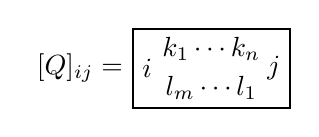
\begin{tikzpicture}
	\draw[thick] (0,0) rectangle (2,1);
	\node[left] at (0,.5) {$[Q]_{ij}=$};
	\node at (1,.75) {$k_1\cdots k_n$};
	\node at (1,.25) {$l_m\cdots l_1$};
	\node[right] at (0,.5) {$i$};
	\node[left] at (2,.5) {$j$};
    	\end{tikzpicture}
	\end{align*}
when $[Q]_{ij}=X_{k_1}\cdots X_{k_n}\otimes X_{l_1}\cdots X_{l_m}$, $i,j\in\{1,\ldots, N\}$.

Lastly, we define the $j$th \textit{$\sigma$-cyclic derivative} $\D_j\colon\mathscr{P}\rightarrow\mathscr{P}$ by
	\begin{equation*}
		\D_j(X_{k_1}\cdots X_{k_n})= \sum_{l=1}^n \alpha_{j k_l} \sigma_{-i}(X_{k_{l+1}}\cdots X_{k_n})X_{k_1}\cdots X_{k_{l-1}}.
	\end{equation*}
$\D_j$ can also be written as $m\circ\diamond\circ(1\otimes\sigma_{-i})\circ\bar{\partial}_j$. Let $\D P=(\D_1 P,\ldots, \D_N P)\in\mathscr{P}^N$ be the \textit{$\sigma$-cyclic gradient}. We also define
	\begin{align*}
		\bar{\D}_j(X_{k_1}\cdots X_{k_n})= \sum_{l=1}^n \alpha_{k_l j} X_{k_{l+1}}\cdots X_{k_n}\sigma_i(X_{k_1}\cdots X_{k_{l-1}}),
	\end{align*}
or $\bar{\D}_j=m\circ\diamond\circ(\sigma_i\otimes 1)\circ\partial_j$. Then $(\D_j P)^*=\bar{\D}_j (P^*)$, and from (\ref{differentiating_sigma}) we also have $\D_j\circ\sigma_i=\bar{\D}_j$.


%	The norm $\|\cdot\|_{R\otimes_\pi R}$
%%%%%%%%%%%%%%%%%%%%%

\subsection{The norm $\|\cdot\|_{R\otimes_\pi R}$.}\label{projective_tensor_norm}

Following \cite{GS14}, we denote by $\|\cdot\|_{R\otimes_\pi R}$ the projective tensor product norm on $\mathscr{P}\otimes \mathscr{P}^{op}$; that is,
	\begin{align*}
		\left\| \sum_i a_i\otimes b_i \right\|_{R\otimes_\pi R} = \sup_{\eta} \left\| \eta\left(\sum_i a_i\otimes b_i\right)\right\|,
	\end{align*}
where the supremum is taken over all maps $\eta$ valued in a Banach algebra such that $\eta(a\otimes 1)$ and $\eta(1\otimes b)$ commute and have norms bounded by $\|a\|_R$ and $\|b\|_R$, respectively. In particular, letting $\eta$ be given by left and right multiplication on $\mathscr{P}$ we see that for $D\in \mathscr{P}\otimes\mathscr{P}^{op}$ and $g\in\mathscr{P}$, we have
	\begin{align*}
		\| D\# g\|_R \leq \|D\|_{R\otimes_\pi R} \|g\|_R.
	\end{align*}
We extend the norm to $\left(\mathscr{P}\otimes\mathscr{P}^{op}\right)^N$ by putting for $F=(F_1,\ldots, F_N)\in \left(\mathscr{P}\otimes\mathscr{P}^{op}\right)^N$
	\begin{align*}
		\|F\|_{R\otimes_\pi R} = \max_{1\leq i \leq n} \|F_i\|_{R\otimes_\pi R}.
	\end{align*}
The same symbol is used to denote the norm imposed on $M_N(\mathscr{P}\otimes\mathscr{P}^{op})$ by identifying it with the Banach space of left multiplication operators on $\left(\mathscr{P}\otimes\mathscr{P}^{op}\right)^N$. In \cite{GS14} it is noted that this norm is given by
	\begin{align*}
		\| Q\|_{R\otimes_\pi R} = \max_{1\leq i\leq N} \sum_{j=1}^N \| [Q]_{ij}\|_{R\otimes_\pi R}.
	\end{align*}

%	Cyclic derivatives of $\sigma$-cyclically symmetric polynomials
%%%%%%%%%%%%%%%%%%%%%%%%%%%

\subsection{Cyclic derivatives of $\sigma$-cyclically symmetric polynomials}

Suppose $g\in\pi_n\left(\mathscr{P}^{(R,\sigma)}_{c.s.}\right)$ and write $g=\sum_{|\ul{j}|=n} c(\ul{j}) X_{\ul{j}}$. Then the condition $\rho^l(g)=g$ for $l\in \{0,\ldots, n-1\}$ implies
	\begin{align*}
		 g&=\rho^l(g)=\sum_{\substack{|\ul{j}|=n-l\\ |\ul{k}|=l}} c(\ul{j}\cdot \ul{k}) \sigma_{-i}(X_{\ul{k}})X_{\ul{j}} \\
		 	&= \sum_{\substack{|\ul{j}|=n-l\\ |\ul{k}|=l}} c(\ul{j}\cdot \ul{k})\sum_{|\ul{i}|=l} A(\ul{k},\ul{i}) X_{\ul{i}}X_{\ul{j}} = \sum_{\substack{|\ul{i}|=l\\ |\ul{j}|=n-l}} \left\{ \sum_{|\ul{k}|=l} c(\ul{j}\cdot \ul{k})A(\ul{k},\ul{i})\right\} X_{\ul{i}}X_{\ul{j}}.
	\end{align*}
Hence
	\begin{align}\label{cyclically_symmetric_coefficients_positive}
		c(\ul{i}\cdot\ul{j})=\sum_{|\ul{k}|=l} c(\ul{j}\cdot \ul{k}) A(\ul{k},\ul{i}).
	\end{align}
A similar computation using $l\in \{-n+1,\ldots, -1,0\}$ yields
	\begin{align}\label{cyclically_symmetric_coefficients_negative}
		c(\ul{i}\cdot\ul{j})=\sum_{|\ul{k}|=l} c(\ul{k}\cdot\ul{i}) A^{-1}(\ul{k}\cdot\ul{j}).
	\end{align}
Since $\rho^n(g)=\sigma_{-i}(g)$ for $g\in\pi_n(\mathscr{P})$, we can use Equation (\ref{cyclically_symmetric_coefficients_positive}) to characterize the coefficients of $g\in \pi_n\left(\mathscr{P}_\varphi\right)$:
	\begin{align}\label{centralizer_coefficients}
		c(\ul{i})=\sum_{|\ul{k}|=n} c(\ul{k}) A(\ul{k},\ul{i}).
	\end{align}
With these formulas in hand, the following lemmas are easily obtained.

\begin{lem}\label{cyclic_derivative_bounded}
For $P = \sum_{|\ul{i}|=n}c(\ul{i})X_{\ul{i}} \in \pi_n\left(\mathscr{P}_{c.s.}\right)$ and each $t\in\{1,\ldots, N\}$ we have
	\begin{equation}\label{cyclic_derivative_of_cyclically_symmetric}
		\D_t \Sigma P=\sum_{|\ul{i}|=n} \alpha_{t i_n} c(\ul{i}) X_{i_1}\cdots X_{i_{n-1}}.
	\end{equation}
Moreover, $\D\Sigma$ can be extended to a bounded operator $\D\Sigma\colon \mathscr{P}_{c.s.}^{(R,\sigma)}\rightarrow \left(\mathscr{P}^{(R)}\right)^N$ with $\|\D\Sigma \|\leq \frac{1}{R}$. Additionally, for $1<S<R$, $\D$ can be extended to a bounded operator $\D\colon \mathscr{P}_{c.s.}^{(R,\sigma)}\rightarrow \left(\mathscr{P}^{(S)}\right)^N$ with $\|\D\| \leq C\left(\frac{R}{S}\right)$ depending only on the ratio $\frac{R}{S}$.
\end{lem}
\begin{proof}
Let $P=\sum_{|\ul{i}|=n} c(\ul{i}) X_{\ul{i}}$. Equation (\ref{cyclic_derivative_of_cyclically_symmetric}) follows easily from Equation (\ref{cyclically_symmetric_coefficients_positive}), which then implies
	\begin{align*}
		\| \D_t\Sigma P\|_R= \left\| \sum_{|\ul{i}|=n} \alpha_{t i_n} c(\ul{i}) X_{i_1}\cdots X_{i_{n-1}}\right\|_R \leq \sum_{|\ul{i}|=n} |c(\ul{i})| R^{n-1} = \frac{1}{R} \|P\|_{R}=\frac{1}{R} \|P\|_{R,\sigma}.
	\end{align*}
So for arbitrary $P\in \mathscr{P}_{c.s.}$ we have
	\begin{align*}
		\| \D\Sigma P\|_R =\max_{t\in\{1,\ldots,N\}} \|\D_t\Sigma P\|_R &\leq \sum_{n=0}^{\deg{P}} \max_{t\in\{1,\ldots,N\}} \|\D_t\Sigma \pi_n(P)\|_R \\
			&\leq \sum_{n=0}^{\deg{P}} \frac{1}{R} \|\pi_n(P)\|_{R,\sigma} = \frac{1}{R} \|P\|_{R,\sigma},
	\end{align*}
and so $\D\Sigma$ extends to $\mathscr{P}_{c.s.}^{(R,\sigma)}$ with the claimed bound on its norm.\par
Considering only $\D$,  (\ref{cyclic_derivative_of_cyclically_symmetric}) implies
	\begin{align*}
		\D_t  P=n\sum_{|\ul{i}|=n} \alpha_{t i_k} c(\ul{i}) X_{i_1}\cdots X_{i_{n-1}}
	\end{align*}
for $P\in\pi_n\left(\mathscr{P}_{c.s.}\right)$. Hence
	\begin{align*}
		\| \D P\|_S \leq n \sum_{|\ul{i}|=n} |c(\ul{i})| S^{n-1} = n\left(\frac{S}{R}\right)^{n-1} \sum_{|\ul{i}|=n} |c(\ul{i})| R^{n-1} = \frac{ n S^{n-1}}{R^n} \|P\|_{R,\sigma}.
	\end{align*}
A routine computation shows for each $n$
	\begin{align*}
		\frac{ n S^{n-1}}{R^n} \leq \frac{ c S^{c-1}}{R^c}\leq c\left(\frac{S}{R}\right)^c=:C\left(\frac{R}{S}\right),
	\end{align*}
where $c=\frac{1}{\ln(R/S)}$. The rest of the argument then proceeds as in the previous case.
\end{proof}

\begin{lem}\label{D_of_S}
For $P\in\mathscr{P}_{\varphi}^{(R,\sigma)}$
	\begin{equation*}
		\D\mathscr{S}\Pi P=\D P.
	\end{equation*}
\end{lem}
\begin{proof}
Suppose $P\in \pi_n(\mathscr{P}_\varphi)$. The cases $n=0,1$ are clear so suppose $n\geq 2$. Write $P=\sum_{|\ul{i}|=n} c(\ul{i}) X_{\ul{i}}$, then
	\begin{align*}
		\mathscr{S}\Pi P&=\frac{1}{n}\sum_{l=0}^{n-1} \sum_{\substack{|\ul{j}|=n-l\\ |\ul{k}|=l}}c(\ul{j}\cdot \ul{k})\sigma_{-i}(X_{\ul{k}}) X_{\ul{j}} = \frac{1}{n}\sum_{l=0}^{n-1} \sum_{\substack{|\ul{i}|=l\\ |\ul{j}|=n-l}} \sum_{|\ul{k}|=l} c(\ul{j}\cdot \ul{k}) A(\ul{k},\ul{i}) X_{\ul{i}} X_{\ul{j}}\\
			&=\frac{1}{n}\sum_{|\ul{i}|=n} \left\{ \sum_{l=0}^{n-1}\sum_{|\ul{k}|=l} c\left( (i_{l+1},\ldots, i_{n})\cdot \ul{k}\right) A\left(\ul{k}, (i_1,\ldots, i_l) \right) \right\} X_{\ul{i}} =: \frac{1}{n} \sum_{|\ul{i}|=n} b(\ul{i}) X_{\ul{i}}.
	\end{align*}
So if we let $Q=\sum_{|\ul{i}|=n} b(\ul{i}) X_{\ul{i}}$, then $\mathscr{S}\Pi P=\Sigma Q$ and using Equation (\ref{cyclic_derivative_of_cyclically_symmetric}) we obtain
	\begin{align*}
		\D_t\mathscr{S}\Pi P=\sum_{|\ul{i}|=n} \alpha_{t i_n} b(\ul{i}) X_{i_1}\cdots X_{i_{n-1}},
	\end{align*}
for each $t\in\{1,\ldots, N\}$. It is then a straightforward computation to show that the above equals $\D_t P$. The case for general $P\in\mathscr{P}_\varphi^{(R,\sigma)}$ then follows from linearity.
\end{proof}

%	Notation
%%%%%%%%

\subsection{Notation}

We use the same notation as in \cite{GS14}, adjusted slightly to accommodate our new operators. For $Q\in M_{N}(\mathscr{P}\otimes \mathscr{P}^{op})$ we write
	\begin{align*}
		\text{Tr}(Q)&=\sum_{i=1}^N [Q]_{ii} \in\mathscr{P}\otimes\mathscr{P}^{op},\\
		\text{Tr}_{A}(Q)&=\text{Tr}(A\# Q) = \sum_{i,j=1}^N [A]_{ij} [Q]_{ji} \in \mathscr{P}\otimes\mathscr{P}^{op},\\
		\text{Tr}_{A^{-1}}(Q) &= \text{Tr}(A^{-1}\# Q) = \sum_{i,j=1}^N [A^{-1}]_{ij} [Q]_{ji}\in\mathscr{P}\otimes\mathscr{P}^{op}.
	\end{align*}
By Corollary \ref{difference_quotient_adjoint} $\mathscr{P}\otimes\mathscr{P}^{op}\subset \dom{\partial_j^*}$, so we note
	\begin{align*}
		\J_\sigma^*(Q)=\left( \sum_i \partial_i^*([Q]_{ji})\right)_{j=1}^N \in L^2(\mathscr{P},\varphi)^N.
	\end{align*}
where $\J_\sigma$ is viewed as a densely defined operator from $L^2(\mathscr{P}^N,\varphi)$ to $L^2(M_N(\mathscr{P}\otimes \mathscr{P}^{op}), \varphi\otimes\varphi^{op}\otimes\text{Tr})$ and the above is its adjoint.

%	Transport and invertible power series
%%%%%%%%%%%%%%%%%%%%

\subsection{Transport and invertible power series}

Let $(\M,\theta)$ be a von Neumann algebra with faithful normal state $\theta$ and let $T_1,\ldots, T_N\in \M$ be self-adjoint elements which generate $\M$. Then, after \cite{GS14}, $\M$ can be thought of as a completion of the algebra $\C\<T_1,\ldots, T_N\>$, and $\theta$ induces a linear functional $\theta_T$ on $\C\<t_1,\ldots, t_N\>$, the non-commutative polynomials in abstract indeterminates $t_1,\ldots, t_N$, via $\theta_T(t_{k_1}\cdots t_{k_n})=\theta(T_{k_1}\cdots T_{k_n})$, $k_1,\ldots, k_n\in\{1,\ldots, N\}$. $\theta_T$ is called the \textit{non-commutative law of} $T_1,\ldots, T_N$ and we write $W^*(\theta_T)\cong \M$. Let $S_1,\ldots, S_N\in \mc{N}$ be self-adjoint elements generating another von Neumann algebra $\mc{N}$ with faithful normal state $\psi$ and let $\psi_S$ be their law so that $W^*(\psi_S)\cong \mc{N}$. 

\begin{defi}\label{transport}
By \textit{transport} from $\theta_T$ to $\psi_S$ we mean an $N$-tuple of self-adjoint elements $Y_1,\ldots, Y_N\in \M$ having the same law as $S_1,\ldots,S_N$:
	\begin{align*}
		\psi(P(S_1,\ldots, S_N)) = \theta(P(Y_1,\ldots, Y_N)),
	\end{align*}
for all non-commutative polynomials $P$ in $N$ variables. If such an $N$-tuple exists then there is a state-preserving embedding $\mc{N}\cong W^*(Y)\subset \M$.
\end{defi}

Let $M=W^*(X_1,\ldots, X_N)$ be as before. Suppose $L$ is a von Neumann algebra generated by self-adjoint $Z_1,\ldots, Z_N$ with faithful normal state $\psi$ and there exists transport $Y=(Y_1,\ldots, Y_N)$  from $\varphi_X$ to $\psi_Z$ such that $Y=G(X)\in (\mathscr{P}^{(R)})^N$. That is, $Y_j=G_j(X)$ is a power series in terms of $X_1,\ldots, X_N$. If we can invert this power series so that $X=H(Y)$, then $H(Z)\in L^N$ is transport from $\psi_Z$ to $\varphi_X$. It would then follow that we have a state-preserving isomorphism $L\cong M$. The following lemma, which is presented as Corollary 2.4 in \cite{GS14}, shows that such inverses can be found.

\begin{lem}\label{invertible_power_series}
Let $R<S$ and consider the equation $Y=X+f(X)$ with $f\in (\mathscr{P}^{(S)})^N$ and $\|Y\|_{R}<S$. Let $R'=\max\{R,\|Y\|_R\}<S$. Then there exists a constant $C>0$, depending only on $S$ and $R$ so that whenever $\|f\|_S<C$, then there exists $H\in (\mathscr{P}^{(R')})^N$ so that $X=H(Y)$.
\end{lem}
\begin{proof}
Fix $S'\in (R', S)$ and define
	\begin{align*}
		C(S')=\|f\|_S \max_{k\geq 0} k(S')^{k-1}S^{-k}.
	\end{align*}
Since $\|f\|_S<C$, we can choose $C$ sufficiently small so that $C(S')<1$ and
	\begin{align*}
		R'+\frac{C}{1-C(S')}\leq S'.
	\end{align*}
We define a sequence of $N$-tuples of (a priori formal) power series with $H^{(0)}=X$ and
	\begin{align*}
		H^{(k)}= X- f(H^{(k-1)})\qquad \forall k\geq 1.
	\end{align*}
We claim that $H^{(k)}\in (\P^{(R')})^N$ with $\|H^{(k)}\|_{R'}<S'$ for each $k\geq 0$. Indeed, this is clearly true for $H^{(0)}$ so assume it holds for $H^{(1)},\ldots, H^{(k-1)}$. Denote the component functions of $H^{(k)}$ by $H^{(k)}_j$ for $j=1,\ldots, N$. Suppose
	\begin{align*}
		f_j(X_1,\ldots, X_N)=\sum_{|\ul{i}|\geq 0} c(\ul{i}) X_{\ul{i}}.
	\end{align*}
Then for any $0\leq l\leq k-1$ we have
	\begin{align*}
		\|H^{(l+1)}_j - H^{(l)}_j\|_{R'} &= \| f_j(H^{(l)}) - f_j(H^{(l-1)})\|_{R'} \\
			&\leq \sum_{n=0}^\infty \sum_{|\ul{i}|=n} |c(\ul{i})| \sum_{u=1}^n \| H^{(l)}\|_{R'}^{u-1} \| H^{(l)}_{i_u} - H^{(l-1)}_{i_u}\|_{R'} \| H^{(l-1)}\|_{R'}^{n-u}\\
			&\leq\|H^{(l)} - H^{(l-1)}\|_{R'}\sum_{n=0}^\infty n(S')^{n-1}S^{-n}\sum_{|\ul{i}|=n} |c(\ul{i})| S^n\\
			&\leq \|H^{(l)} - H^{(l-1)}\|_{R'} C(S').
	\end{align*}
As $j$ was arbitrary, we obtain through iteration
	\begin{align*}
		\|H^{(l+1)} - H^{(l)}\|_{R'} \leq \|H^{(1)} - H^{(0)}\|_{R'} C(S')^l = \| f\|_{R'} C(S')^l \leq C C(S')^l,
	\end{align*}
and thus
	\begin{align*}
		\| H^{(k)}\|_{R'} &\leq \|H^{(0)}\|_{R'} + \|H^{(k)}- H^{(0)}\|_{R'} \\
				&\leq R' + \sum_{l=0}^{k-1} \|H^{(l+1)} - H^{(l)}\|_{R'} \\
				&\leq R' + \sum_{l=0}^{k-1} C C(S')^l \\
				&\leq R' + \frac{C}{1 - C(S')} \leq S',
	\end{align*}
by our assumption on $C$. So the claim holds and by induction we have the bound $\|H^{(k)}\|_{R'}\leq S'$ for all $k\geq 0$. Moreover, by a standard argument we can see that $\{H^{(k)}\}_{k\geq 0}$ is a Cauchy sequence and so converges to some $H\in (\P^{(R')})^N$ satisfying $\|H\|_{R'}\leq S'$ and $H=X-f(H)$.

Now, $Y=X+f(X)$ satisfies $\|Y\|_R\leq R'$ and so $H(Y)\in (\P^{(R)})^N$ with $\|H(Y)\|_R \leq S'$ and $H(Y)=Y- f(H(Y))$. Since $\|X\|_R=R\leq S'$ we can use the same argument as above to show
	\begin{align*}
		\| X- H(Y)\|_R = \| Y - f(X) - Y+ f(H(Y))\|_R \leq \| X - H(Y)\|_R C(S').
	\end{align*}
But $C(S')<1$ implies $H(Y)=X$.
\end{proof}


%	Monotonicity of transport
%%%%%%%%%%%%%%%

\subsection{Monotonicity of transport.}

We introduce a definition for what it means for transport to be ``monotone.\rq{}\rq{} Note that in the tracial case ($A=1$) this coincides with Definition 2.1 in \cite{GS14}.
\begin{defi}
We say that transport from $\varphi_X$ to $\psi_Z$ via the $N$-tuple $Y=(Y_1,\ldots, Y_N)$ is monotone if $Y=\D G$ for some $G\in \mathscr{P}^{(R)}$, $R\geq4\sqrt{\|A\|}$, such that $(\sigma_\frac{i}{2}\otimes 1)(\J_\sigma \D G)\geq 0$ as an operator on $L^2(\mathscr{P}\otimes\mathscr{P}^{op},\varphi\otimes\varphi^{op})^N$.
\end{defi}

Suppose $(\M,\psi)$ is a von Neumann algebra with a faithful normal state $\psi$. Let $\H_\psi=L^2(\M,\psi,\xi_0)$ be the Hilbert space obtained via the GNS construction with a cyclic vector implementing $\psi$. Let $S_\psi$ be the Tomita conjugation for the left Hilbert algebra $\M\xi_0$, and let $\Delta_\psi$ and $J_\psi$ be the modular operator and conjugation (respectively). Recall (\emph{cf.} \cite{Tak03}, Chapter IX, \textsection 1) that there is a canonical pointed convex cone
	\begin{align*}
		\mathfrak{P}_\psi=\overline{\{ \Delta_\psi^{1/4}x\xi_0\colon x\in\M_+\}}^{\|\cdot\|_{\psi}},
	\end{align*}
which is self-dual in the sense that if $\eta\in\H_\psi$ satisfies $\<\eta,\xi\>_\psi\geq 0$ for all $\xi\in \mf{P}_\psi$ then $\eta\in \mf{P}_\psi$. The embedding
	\begin{align*}
		x\mapsto \Delta_\psi^\frac{1}{4} x \xi_0
	\end{align*}
of $\M$ into $\H_\psi$ then has the benefit of sending positive elements in $\M$ into $\mf{P}_\psi$.\par
In particular, if $\M=M_N(M\bar{\otimes} M^{op})$ and $\psi=\varphi\otimes\varphi^{op}\otimes \text{Tr}_A$ then
	\begin{align*}
		\Delta_\psi^\frac{1}{4} q \xi_0= (\sigma_{-\frac{i}{4}}\otimes \sigma_\frac{i}{4})(A^\frac{1}{4}\# q\# A^{-\frac{1}{4}})\xi_0.
	\end{align*}
We shall see in Lemma \ref{change_of_variables}.(iv) that if $G\in \mathscr{P}_\varphi^{(R,\sigma)}$ then $A^s\#\J_\sigma \D G \# A^{-s}=(\sigma_{-is}\otimes\sigma_{-is})(\J_\sigma \D G)$. Hence if $Y=\D G$ for such $G$, then $(\sigma_\frac{i}{2}\otimes 1)(\J_\sigma Y)$ embeds into $\H_\psi$ as
	\begin{align*}
		(\sigma_{-\frac{i}{4}}\otimes \sigma_\frac{i}{4})(A^\frac{1}{4}\# (\sigma_\frac{i}{2}\otimes 1)(\J_\sigma Y)\# A^{-\frac{1}{4}})\xi_0 = \J_\sigma Y \xi_0.
	\end{align*}



%	The Schwinger-Dyson equation and free Gibbs state
%%%%%%%%%%%%%%%%%%%%%%%%%

\subsection{The Schwinger-Dyson equation and free Gibbs state.}\label{S-D_section}
Our construction of the transport $Y$ will exploit the condition that $\varphi_Y$ satisfies the so-called Schwinger-Dyson equation:

\begin{defi}
Given $V\in\mathscr{P}^{(R,\sigma)}_{c.s.}$, we say a linear functional $\varphi_V$ on $\mathscr{P}$ satisfies \textit{the Schwinger-Dyson equation with potential $V$} if
	\begin{align}\label{Schwinger-Dyson_1}
		\varphi_V( \D(V) \# P) = \varphi_V\otimes\varphi_V^{op}(\text{Tr}(\J_\sigma P)),\qquad\forall P\in\mathscr{P}.
	\end{align}
The law $\varphi_V$ is called the \textit{free Gibbs state with potential $V$}.
\end{defi}

Note that when $\J_\sigma$ is viewed as a densely defined operator from $L^2(\mathscr{P}^N,\varphi)$ to $L^2(M_N(\mathscr{P}\otimes\mathscr{P}^{op}),\varphi\otimes\varphi^{op}\otimes\text{Tr})$, (\ref{Schwinger-Dyson_1}) is equivalent to
	\begin{align}\label{Schwinger-Dyson_2}
		\J_\sigma^*(1)=\D V,
	\end{align}
where $1\in M_N(\mathscr{P}\otimes\mathscr{P}^{op})$ is the identity matrix.\par
Consider the potential
	\begin{align}\label{quadratic_potential}
		V_0=\frac{1}{2}\sum_{j,k=1}^N \left[\frac{1+A}{2}\right]_{jk} X_k X_j.
	\end{align}
Then
	\begin{align*}
		\rho(V_0)&=\frac{1}{2}\sum_{j,k=1}^N  \left[\frac{1+A}{2}\right]_{jk} \sigma_{-i}(X_j)X_k\\
			&=\frac{1}{2}\sum_{j,k,l=1}^N  \left[\frac{1+A^{-1}}{2}\right]_{kj}[A]_{jl} X_l X_k\\
			& = \frac{1}{2} \sum_{k,l=1}^N  \left[\frac{1+A}{2}\right]_{kl} X_l X_k= V_0,
	\end{align*}
and hence $V_0\in\mathscr{P}_{c.s.}^{(R,\sigma)}$. Also,
	\begin{align*}
		\D_l(V_0)&=\frac{1}{2}\sum_{i,j}  \left[\frac{1+A}{2}\right]_{ij} \left(\alpha_{lj} \sigma_{-i}(X_i) + \alpha_{li} X_j\right)\\
			&= \frac{1}{2} \sum_{i,j,k=1}^N  \left[\frac{2}{1+A}\right]_{lj}\left[\frac{1+A^{-1}}{2}\right]_{ji}[A]_{ik} X_k + \frac{1}{2}\sum_{i,j=1}^N  \left[\frac{2}{1+A}\right]_{li} \left[\frac{1+A}{2}\right]_{ij} X_j \\
			&=\frac{1}{2}X_l+\frac{1}{2}X_l=X_l,
	\end{align*}
so that $\D V_0=X$. Using $A=A^*$ it is also easy to see that $V_0^*=V_0$.\par
Now, (\ref{Schwinger-Dyson_2}) for $V=V_0$ states $\J_\sigma^*(1)=X$, or $\partial_j^*(1\otimes 1)=X_j$ for each $j=1,\ldots, N$, where the the adjoint is with respect to $\varphi_{V_0}$. However, from (\ref{adjoint_of_1}) we know this relation holds when the adjoint of $\partial_j=\partial_j^{(0)}$ is taken with respect to the free quasi-free state $\varphi_0$. We therefore immediately obtain the following result.

\begin{thm}\label{free_Gibbs_is_free_quasi-free}
The free Gibbs state with potential $V_0$ is the free quasi-free state $\varphi_0$ on $M_0=\Gamma(\H_\R,U_t)''$.
\end{thm}\par

It is clear that the $\varphi_{V_0}$ is unique since (\ref{Schwinger-Dyson_1}) for $V=V_0$ recursively defines $\varphi_{V_0}$ for all monomials. However, even for small perturbations (in the $\|\cdot\|_{R,\sigma}$-norm) $V=V_0+W$  of $V_0$ the free Gibbs state with potential $V$ is unique, which we demonstrate below. Consequently, if $\psi_Z$ satisfies the Schwinger-Dyson equation for a $V$, then to find transport from $\varphi_X$ it suffices to produce $Y\in M^N$ whose law $\varphi_Y$ (determined by $\varphi$) satisfies the Schwinger-Dyson equation with the same potential $V$. The proof of uniqueness presented here differs from the proof of Theorem 2.1 in \cite{GM06} only in the differential operators considered.


\begin{thm}\label{Gibbs_state_unique}
Fix $R\geq 4\sqrt{\|A\|}$. Let $V=V_0+W\in \mathscr{P}_{c.s.}^{(R,\sigma)}$. Then for sufficiently small $\|W\|_{R,\sigma}$, the Schwinger-Dyson equation has a unique solution amongst states that satisfy
	\begin{align}\label{phi_monomial0}
		|\varphi(X_{\ul{j}})| \leq 3^{|\ul{j}|}
	\end{align}
for any multi-index $\ul{j}$.
\end{thm}
\begin{proof}
Suppose two states $\varphi$ and $\varphi'$ both solve the Schwinger-Dyson equation with potential $V$. Then $\varphi(1)=\varphi'(1)=1$ and hence they agree on $\pi_0(\mathscr{P})$. Fix $l\geq 1$ and a monomial $P\in \pi_{l-1}(\mathscr{P})$. Then we have
	\begin{align*}
		(\varphi-\varphi')(X_i P)= ((\varphi-\varphi')\otimes\varphi)(\partial_i P) + (\varphi'\otimes (\varphi-\varphi'))(\partial_i P) - (\varphi-\varphi')(\D_i W P).
	\end{align*}
(Note that for $l=1$ the first two terms disappear). Define
	\begin{equation*}
		\Delta_l(\varphi,\varphi'):=\max_{|\ul{j}|=l} |(\varphi-\varphi')(X_{\ul{j}})|.
	\end{equation*}
In particular $\Delta_0(\varphi,\varphi')=0$. Write $\D W=\sum_{\ul{i}} c(\ul{j}) X_{\ul{j}}$. Then we have
	\begin{align*}
		\Delta_l(\varphi,\varphi') \leq 2 \sum_{k=0}^{l-2} \Delta_k(\varphi,\varphi') 3^{l-2-k} + \sum_{p=0}^\infty \sum_{|\ul{j}|=p} |c(\ul{j})| \Delta_{p+l-1}(\varphi,\varphi').
	\end{align*}
For $\gamma>0$, set
	\begin{equation*}
		d_\gamma(\varphi,\varphi') = \sum_{l=1}^\infty \gamma^l \Delta_l(\varphi,\varphi').
	\end{equation*}
Since (\ref{phi_monomial0}) implies $\Delta_l(\varphi,\varphi')\leq 2 (3)^l$, we see that $d_\gamma(\varphi,\varphi')<\infty$ so long as $\gamma< \frac{1}{3}$. In the above equality we multiply both sides of the equation by $\gamma^l$ and then sum over $l\geq 1$ to obtain
	\begin{align*}
		d_\gamma&(\varphi,\varphi') \leq 2\sum_{l=2}^\infty \gamma^l\sum_{k=0}^{l-2} \Delta_k(\varphi,\varphi') 3^{l-2-k} + \sum_{l=1}^\infty \gamma^l \sum_{p=0}^\infty \sum_{|\ul{j}|=p} |c(\ul{j})| \Delta_{p+l-1}(\varphi,\varphi')\\
				&=2\gamma^2\sum_{k=0}^\infty \gamma^k\Delta_k(\varphi,\varphi')\sum_{l=k+2}^\infty \gamma^{l-2-k}3^{l-2-k} + \sum_{p=0}^\infty \sum_{|\ul{j}|=p} |c(\ul{j})| \gamma^{-p+1}\sum_{l=1}^\infty \gamma^{p+l-1}\Delta_{p+l-1}(\varphi,\varphi')\\
				&\leq \frac{2\gamma^2}{1-3\gamma} d_\gamma(\varphi,\varphi') + \gamma\sum_{p=0}^\infty \sum_{|\ul{j}|=p} |c(\ul{j})| \gamma^{-p}d_\gamma(\varphi,\varphi').
	\end{align*}
Let $\gamma=\frac{28}{25 R}$. Then $\gamma^{-1}<R$ and $R>4$ implies $3\gamma<\frac{21}{25}$. Hence
	\begin{align*}
		d_\gamma(\varphi,\varphi')&\leq d_\gamma(\varphi,\varphi')\left(\frac{49}{50} + \frac{7}{25}\|\D W\|_{\frac{25R}{28}}\right).
	\end{align*}
Recall from Lemma \ref{cyclic_derivative_bounded}, that $\|\D W\|_{\frac{25R}{28}} \leq C\|W\|_{R,\sigma}$ where the constant only depends on the ratio $\frac{R}{25R/28}=\frac{28}{25}$. Thus if $\|W\|_{R,\sigma} <\frac{1}{14C}$ then
	\begin{align*}
		d_\gamma(\varphi,\varphi') \leq c d_\gamma(\varphi,\varphi')\qquad \text{with }c<1,
	\end{align*}
implying $d_\gamma(\varphi,\varphi')=0$ and hence $\Delta_l(\varphi,\varphi')=0$ for all $l\geq 1$.
\end{proof}

This theorem implies that if the law $\psi_Z$ of $Z=(Z_1,\ldots, Z_N)\subset (L,\psi)$ and the law $\varphi_Y$ of $Y=(Y_1,\ldots, Y_N)\subset (M,\varphi)$ both solve the Schwinger-Dyson equation with potential $V$, then $W^*(Z_1,\ldots, Z_N)\cong W^*(Y_1,\ldots, Y_N)\cong W^*(\varphi_V)$. In particular, $W^*(\varphi_V)$ is well-defined.

%	Outline of the Paper
%%%%%%%%%%%%%

\subsection{Outline of the paper.}

The general outline for the paper is as follows: we begin in Section \ref{construction} by fixing $q=0$ and a potential $V=V_0+W\in \mathscr{P}^{(R,\sigma)}_{c.s.}$ and assuming there exists $Y=(Y_1,\ldots, Y_N)\in (\mathscr{P}^{(R)})^N$ whose law (induced by $\varphi$) satisfies the Schwinger-Dyson equation with potential $V$. Several equivalent versions of this equation will be derived in Sections \ref{equivalent_S-D} and \ref{identities} until we arrive at a final version for which a fixed point argument can be applied. Several technical estimates will be produced in Section \ref{technical_estimates} for the purposes of this fixed point argument so that in Section \ref{existence_of_g}, given certain assumptions regarding $V$, we can assert the existence of $Y$. Having obtained the desired transport, we then use Lemma \ref{invertible_power_series} to refine the transport into an isomorphism in Section \ref{summary}. Finally, in Section \ref{application} we present the main application to q-deformed Araki-Woods algebras.


%%%%%%%%%%%%%%%%%%%%%%%%%%%%%%
%	Construction of the Non-tracial monotone transport map	%
%%%%%%%%%%%%%%%%%%%%%%%%%%%%%%

\section{Construction of the Non-tracial monotone transport map}\label{construction}

For all this section, we consider only $q=0$ and maintain the same notational simplifications as above ($M=M_0$, $\varphi=\varphi_0$, $X_j^{(0)}=X_j$, and $\sigma^{\varphi_0}_{z}=\sigma_z$).  Recall that $V_0$ is defined by (\ref{quadratic_potential}) and that by Theorem \ref{free_Gibbs_is_free_quasi-free}, $\varphi$ is the free Gibbs state with potential $V_0$. Our goal is to construct $Y=(Y_1,\ldots, Y_N)\in (\mathscr{P}^{(R)})^N$ whose law with respect to $\varphi$ is the free Gibbs state with potential $V=V_0+W \in \mathscr{P}^{(R,\sigma)}_{c.s.}$, for $\|W\|_{R,\sigma}$ sufficiently small.\par
We will need differential operators $\partial_j$, $\J_\sigma$, $\J$, and $\D$ for $Y$ as well as $X$, so we adopt the following convention: differential operators which have no indices or have a numeric index refer to differentiation with respect to $X_1,\ldots, X_N$. Operators involving differentiation with respect to $Y_1,\ldots, Y_N$ shall be labeled $\partial_{Y_j}$, $\D_{Y_j}$, etc. We define these latter operators using the comments at the end of Subsection \ref{derivations_on_M_q}; that is, $\partial_{Y_j}(Y_{k_1}\cdots Y_{k_n})$ is computed exactly as one would compute $\partial_j(X_{k_1}\cdots X_{k_n})$ and exchanging $X_j$'s for $Y_j$'s in the end.\par
Assuming the law $\varphi_Y$ of $Y=(Y_1,\ldots, Y_N)$ is the free Gibbs state with potential $V$ and $1\otimes 1\in\dom{\partial_{Y_j}^*}$, (\ref{Schwinger-Dyson_2}) implies
	\begin{equation*}
		\partial_{Y_j}^*(1\otimes 1)=\D_{Y_j} (V_0(Y)+W(Y))=Y_j+\D_{Y_j}(W(Y)),
	\end{equation*}
or, in short
	\begin{align}\label{Schwinger-Dyson_Y}
		(\J_\sigma)_Y^*(1)=Y+(\D W)(Y).
	\end{align}
It will turn out that $Y=X+f$ for some $f=\D g$ and $g\in\mathscr{P}^{(R,\sigma)}_{c.s.}$, and so we start by considering the implications of assuming $Y$ is of this form.


%	Change of variables formula
%%%%%%%%%%%%%%%%

\subsection{Change of variables formula.}

\begin{lem}\label{change_of_variables}
Assume $Y$ is such that $\J_\sigma Y=(\partial_{X_j} Y_i)_{ij}\in M_N(M\bar{\otimes}M^{op})$ is bounded and invertible.
	\begin{enumerate}
	\item[(i)] Define
		\begin{equation*}
			\hat{\partial}_j(P)=\sum_{i=1}^N \partial_{X_i}(P)\#\left[ \J_\sigma Y^{-1}\# \J_\sigma X\right]_{ij},
		\end{equation*}
	then $\hat{\partial}_j=\partial_{Y_j}$.
	
	\item[(ii)] $\partial_{Y_j}^*(1\otimes 1)=\sum_l \partial_{X_l}^*\circ\hat{\sigma}_{-i}\left(\left[ \J_\sigma Y^{-1}\# \J_\sigma X\right]_{lj}^*\right)$. Hence
		\begin{equation}\label{change_of_variables_formula}
			(\J_\sigma)_Y^*(1)=\J_\sigma^*\left(\hat{\sigma}_{-i}\left( \J_\sigma X\# \left(\J_\sigma Y^{-1}\right)^*\right)\right),
		\end{equation}
	where $1\in M_N(M\bar{\otimes}M^{op})$ is the identity matrix.

	\item[(iii)] Assume in addition that $Y_j=\D_jG$ for some $G\in\mathscr{P}^{(R,\sigma)}_\varphi$ with $G=G^*$. Then $(\J_\sigma Y)^*=(\sigma_i\otimes 1)(\J_\sigma Y)$ and $\left(\J_\sigma Y^{-1}\right)^*=(\sigma_i\otimes 1)(\J_\sigma Y^{-1})$ and hence Equation (\ref{change_of_variables_formula}) becomes
		\begin{equation}\label{change_of_variables_formula_2}
			(\J_\sigma)_Y^*(1)=\J_\sigma^*\circ (1\otimes \sigma_i)\left( \J_\sigma X \# \J_\sigma Y^{-1}\right).
		\end{equation}
	
	\item[(iv)] For $G\in\mathscr{P}^{(R,\sigma)}_{\varphi}$,
		\begin{align*}
			(\sigma_{-is}\otimes\sigma_{-is})(\J_\sigma\D G) = A^s\# \J_\sigma\D G \# A^{-s},\qquad \forall s\in\R.
		\end{align*}
	\end{enumerate}
\end{lem}
\begin{proof}
Let $Q=\J_\sigma Y$.
	\begin{enumerate}
	\item[(i):] We verify
		\begin{align*}
			\hat{\partial}_iY_k&=\sum_{i=1}^N \partial_{X_i}Y_k\#[Q^{-1}\# \J_\sigma X]_{ij}=\sum_{i=1}^N Q_{ki}\#[Q^{-1}\#\J_\sigma X]_{ij}\\
				&=[Q\#Q^{-1}\#\J_\sigma X]_{kj}=[\J_\sigma X]_{kj}=\partial_{X_j}X_k=\alpha_{kj}1\otimes 1=\partial_{Y_j}Y_k.
		\end{align*}
		
	\item[(ii):] We compute
		\begin{align*}
			\<\partial_{Y_j}^*(1\otimes 1), X_{k_1}\cdots X_{k_p}\>_\varphi &= \<1\otimes 1, \partial_{Y_j}(X_{k_1}\cdots X_{k_p})\>_{\varphi\otimes\varphi^{op}}\\
							&=\sum_{l=1}^N \<1\otimes 1, \partial_{X_l}(X_{k_1}\cdots X_{k_p})\#[Q^{-1}\#\J_\sigma X]_{lj}\>_{\varphi\otimes\varphi^{op}}\\
							&=\sum_{l=1}^N \<\hat{\sigma}_{-i}\left([Q^{-1}\# \J_\sigma X]_{lj}^*\right), \partial_{X_l}(X_{k_1}\cdots X_{k_p})\>_{\varphi\otimes\varphi^{op}}\\
							&=\< \sum_{l=1}^N \partial_{X_l}^*\circ \hat{\sigma}_{-i}\left([Q^{-1}\# \J_\sigma X]_{lj}^*\right),X_{k_1}\cdots X_{k_p}\>_\varphi.
		\end{align*}
		 Recalling that $\J_\sigma X=\J_\sigma X^*$, the definition of $\J_\sigma^*$ implies (\ref{change_of_variables}).
		 
	\item[(iii):] Suppose $G=G^*\in\mathscr{P}^{(R,\sigma)}_{\varphi}$. Then 
		\begin{equation*}
			[(\J_\sigma\D G)^*]_{jk}=[\J_\sigma\D G]_{kj}^*=\partial_j\circ\D_k(G)^*=\tilde{\partial}_j\circ\bar{\D}_k(G^*)=\tilde{\partial}_j\circ\bar{\D}_k(G).
		\end{equation*}		
	A computation on monomials shows that
		\begin{align*}
			\left[\tilde{\partial}_j\circ\bar{\D}_k-(\sigma_i\otimes 1)\circ\partial_k\circ\D_j\right]\circ\sigma_{it}(P)=H_t(P)-H_{t-1}(P),
		\end{align*}
	where
		\begin{align*}
			H_t(P)=\sum_{a,b=1}^N \sum_{P=AX_bB X_a C}\left[\frac{2A^t}{1+A^{-1}}\right]_{ka}\left[\frac{2A^{t+1}}{1+A}\right]_{jb} \sigma_{i(t+1)}(B)\otimes \sigma_{it}(C)\sigma_{i(t+1)}(A).
		\end{align*}
	We claim that $H_{t-1}(P)=H_t(\sigma_{-i}(P))$. Indeed
	\begin{align*}
		H_{t-1}(P)=&\sum_{a,b=1}^N \sum_{P=AX_bBX_aC} \sum_{p,q=1}^N \left[\frac{2 A^t}{1+A^{-1}}\right]_{kp}[A^{-1}]_{pa}\left[\frac{2A^{t+1}}{1+A}\right]_{jq}[A^{-1}]_{qb}\\
				&\times \sigma_{i(t+1)}( \sigma_{-i}(B))\otimes \sigma_{it}(\sigma_{-i}(C)) \sigma_{i(t+1)}(\sigma_{-i}(A))\\
 =& \sum_{a,b,p,q=1}^N [A^{-1}]_{pa}[A^{-1}]_{qb}\sum_{P=\sigma_i(A)X_l\sigma_i(B)X_k\sigma_i(C)} \left[\frac{2 A^t}{1+A^{-1}}\right]_{kp} \left[\frac{2A^{t+1}}{1+A}\right]_{jq}\\
 				&\times \sigma_{it(t+1)}(B)\otimes \sigma_{it}(C)\sigma_{i(t+1)}(A).
	\end{align*}
Note that $\sigma_i(X_p)=\sum_{a=1}^N [A^{-1}]_{pa} X_a$ and $\sigma_i(X_q)=\sum_{b=1}^N [A^{-1}]_{qb} X_b$. So continuing the above computation we have
	\begin{align*}
		H_{t-1}(P)&=\sum_{p,q=1}^N \sum_{P=\sigma_i(AX_pBX_qC)} \left[\frac{2 A^t}{1+A^{-1}}\right]_{kp} \left[\frac{2A^{t+1}}{1+A}\right]_{jq} \sigma_{it(t+1)}(B)\otimes \sigma_{it}(C)\sigma_{i(t+1)}(A)\\
				&=\sum_{p,q=1}^N \sum_{\sigma_{-i}(P)=AX_pBX_qC} \left[\frac{2 A^t}{1+A^{-1}}\right]_{kp} \left[\frac{2A^{t+1}}{1+A}\right]_{jq} \sigma_{it(t+1)}(B)\otimes \sigma_{it}(C)\sigma_{i(t+1)}(A)\\
				&=H_t(\sigma_{-i}(P)).
	\end{align*}
Thus from $G=\sigma_{-i}(G)$ we obtain
	\begin{align*}
		\left[\tilde{\partial}_j\circ\bar{\D}_k-(\sigma_i\otimes 1)\circ\partial_k\circ\D_j\right]\circ\sigma_{it}(G)=0,
	\end{align*}
and hence
	\begin{align*}
		(\J_\sigma \D G)^*=(\sigma_i\otimes 1)(\J_\sigma\D G).
	\end{align*}
	Now, if $Y=\D G$ for such $G$ then $\J_\sigma Y^*=(\sigma_i\otimes 1)(\J_\sigma Y)$ and $\J_\sigma Y^{-1}$ satisfies this formula as well because $\sigma_i\otimes 1$ is a homomorphism. That Equation (\ref{change_of_variables_formula}) becomes Equation (\ref{change_of_variables_formula_2}) is then clear after realizing $\J_\sigma X=(\sigma_{it} \otimes \sigma_{is})(\J_\sigma X)$  for all $t,s\in \R$ (since the entries of $\J_\sigma X$ are merely scalars multiplied with $1\otimes 1$).
	
	\item[(iv):] Recall
		\begin{align*}
			(\sigma_{-it}\otimes\sigma_{-it})\circ\partial_j\circ\sigma_{it} = \sum_{k=1}^N [A^{-t}]_{kj} \partial_k.
		\end{align*}
	Also,
		\begin{align*}
			\bar{\partial}_j=(\sigma_i\otimes\sigma_i)\circ\partial_j\circ\sigma_{-i},
		\end{align*}
	so that
		\begin{align*}
			(\sigma_{-it}\otimes\sigma_{-it})\circ\bar{\partial}_j\circ\sigma_{it}=\sum_{k=1}^N [A^{-t}]_{kj}\bar{\partial}_k.
		\end{align*}
	Using these identities we have
		\begin{align*}
			(\sigma_{-is}\otimes\sigma_{-is})\circ \partial_k\circ \D_j &= (\sigma_{-is}\otimes\sigma_{-is})\circ\partial_k\circ m \circ\diamond\circ(1\otimes\sigma_{-i})\circ\bar{\partial}_j\\
							&=\sum_{a,b=1}^N [A^{-s}]_{ak}[A^{-s}]_{bj} \partial_a\circ m\circ\diamond\circ(1\otimes\sigma_{-i})\circ \circ\bar{\partial}_b\circ\sigma_{-is}\\
							&=\sum_{a,b,=1}^N [A^{s}]_{jb} [A^{-s}]_{ak}  \partial_a\circ\D_b\circ\sigma_{-is}.
		\end{align*}
	Hence for $G\in\mathscr{P}_\varphi^{(R,\sigma)}$ we have
		\begin{align*}
			[(\sigma_{-is}\otimes\sigma_{-is})(\J_\sigma \D G)]_{jk}&=(\sigma_{-is}\otimes\sigma_{-is})\circ \partial_k\circ \D_j(G)\\
				&=\sum_{a,b,=1}^N [A^s]_{jb} [A^{-s}]_{ak} \partial_a\circ\D_b\circ\sigma_{-is}(G)\\
				&=\sum_{a,b,=1}^N [A^s]_{jb} [A^{-s}]_{ak} [\J_\sigma\D G]_{ba} = [A^s\# \J_\sigma\D G\# A^{-s}]_{jk},
		\end{align*}
	for each $j,k=1,\ldots, N$.\qedhere
	\end{enumerate}
\end{proof}

\begin{cor}
Assume $g=g^*\in\mathscr{P}^{(R,\sigma)}_{\varphi}$ and put $G=V_0+g$ and $f_j=\D_j g$. Let $Y_j=X_j+f_j$ so that $Y=\D G$. Define $B=\J_\sigma f\# \J_\sigma X^{-1}$ and assume $1+B$ is invertible. Then Equation (\ref{Schwinger-Dyson_Y}) is equivalent to the equation
	\begin{equation}\label{S-D_Y_2}
		\J_\sigma^*\circ(1\otimes\sigma_i)\left( \frac{1}{1+B}\right) = X+f+(\D W)(X+f).
	\end{equation}
\end{cor}
\begin{proof}
Since $\J_\sigma X+ \J_\sigma f=(1+B)\#\J_\sigma X$, $\J_\sigma Y=\J_\sigma X+\J_\sigma f$ is invertible as a consequence of $1+B$ and $\J_\sigma X$ both being invertible. Then upon noting that
	\begin{equation*}
		\J_\sigma X\# (\J_\sigma X+ \J_\sigma f)^{-1}= 1\# (1+B)^{-1}=\frac{1}{1+B},
	\end{equation*}
the corollary follows immediately from Lemma \ref{change_of_variables}, (ii) and (iii).
\end{proof}


%	An equivalent form of Equation (\ref{S-D_Y_2})
%%%%%%%%%%%%%%%%%%%%%%%%%

\subsection{An equivalent form of Equation (\ref{S-D_Y_2})}\label{equivalent_S-D}

\begin{lem}\label{K_1}
Assume that the map $\xi\mapsto (1+B)\# \xi$ is invertible on $\left(\mathscr{P}^{(R)}\right)^N$, and that $f=\D g$ for some self-adjoint $g\in\mathscr{P}_\varphi^{(R,\sigma)}$. Let
	\begin{equation*}
		K(f)=-\J_\sigma^*\circ(1\otimes \sigma_i)(B)- f.
	\end{equation*}
Then Equation (\ref{S-D_Y_2}) is equivalent to
	\begin{align*}
		K(f)=&\D(W(X+f))\\
			&+\left[B\# f+ B\#\J_\sigma^*\circ(1\otimes\sigma_i)\left(\frac{B}{1+B}\right) -\J_\sigma^*\circ(1\otimes\sigma_i)\left(\frac{B^2}{1+B}\right)\right].
	\end{align*}
\end{lem}
\begin{proof}
Using $\frac{1}{1+x}=1-\frac{x}{1+x}$ and $\J_\sigma^*\circ(1\otimes \sigma_i)(1)=\J_\sigma^*(1)=X$, we see that Equation (\ref{S-D_Y_2}) is equivalent to
	\begin{align*}
		0=\J_\sigma^*\circ(1\otimes\sigma_i)\left(\frac{B}{1+B}\right)+f+(\D W)(X+f).
	\end{align*}
By the assumed invertibility of multiplying by $(1+B)$, this is then equivalent to
	\begin{align*}
		0=&\J_\sigma^*\circ(1\otimes\sigma_i)\left(\frac{B}{1+B}\right)+f+(\D W)(X+f)\\
			&+B\#\J_\sigma^*\circ(1\otimes\sigma_i)\left(\frac{B}{1+B}\right)+B\#f+B\#(\D W)(X+f).
	\end{align*}
Using $\frac{x}{1+x}=x-\frac{x^2}{1+x}$, we then obtain
	\begin{align*}
		K(f)=&(\D W)(X+f)+B\#(\D W)(X+f) \\
			&+\left[B\# f+ B\#\J_\sigma^*\circ(1\otimes\sigma_i)\left(\frac{B}{1+B}\right)-\J_\sigma^*\circ(1\otimes\sigma_i)\left(\frac{B^2}{1+B}\right)\right].
	\end{align*}
Thus it remains to show
	\begin{align*}
		\D_j (W(X+f)) = [(1+B)\# (\D W)(X+f)]_j,
	\end{align*}
for each $j=1,\ldots,N$. Initially suppose $W=X_{k_1}\cdots X_{k_n}$ (the general case will follow via linearity), then
	\begin{align*}
		W(X+f)= (X_{k_1}+f_{k_1})\cdots (X_{k_n}+f_{k_n}).
	\end{align*}
For notational convenience, if we are focusing on the $k_l$th factor then we will write $W(X+f)=A_l(X_{k_l}+f_{k_l})B_l$. Using the derivation property of $\bar{\partial}_j$ in $\D_j=m\circ\diamond\circ(1\otimes\sigma_{-i})\circ\bar{\partial}_j$ we have
	\begin{align*}
		\D_j(W(X+f))=&\sum_{l=1}^n m\circ\diamond\circ(1\otimes \sigma_{-i})\left[ A_l (\alpha_{jk_l}1\otimes 1+\bar{\partial}_j(f_{k_l}) )B_l\right]\\
				=&\sum_{l=1}^n  \alpha_{j k_l} \sigma_{-i}(B_l)A_l + (1\otimes\sigma_{-i})\circ\bar{\partial}_j(f_{k_l})^\diamond\# \sigma_{-i}(B_l)A_l\\
				=&(\D W)(X+f)+\sum_{l=1}^n \partial_{k_l}(f_j)\#\sigma_{-i}(B_l)A_l,
	\end{align*}
where we have used $(\J_\sigma f)^*=(\J_\sigma\D g)^*=(\sigma_i\otimes 1)(\J_\sigma\D g)=(\sigma_i\otimes 1)(\J_\sigma f)$. Now
	\begin{align*}
		[&B\# (\D W)(X+f)]_j\\
			&=\sum_{k=1}^N [B]_{jk}\# (\D_k W)(X+f)=\sum_{k=1}^N \sum_{l=1}^N [\J_\sigma f]_{jl}\# [\J_\sigma X^{-1}]_{lk}\# (\D_k W)(X+f)\\
				&= \sum_{l=1}^N [\J_\sigma f]_{jl}\#\sum_{k=1}^N [\J_\sigma X^{-1}]_{lk} \sum_{p=1}^N \alpha_{kp}\ m\circ\diamond\circ(1\otimes\sigma_{-i})\circ\delta_p (W)(X+f)\\
				&=\sum_{l=1}^N [\J_\sigma f]_{jl}\# m\circ\diamond\circ(1\otimes\sigma_{-1})\circ\delta_l(W)(X+f)=\sum_{l=1}^n [\J_\sigma f]_{j k_l}\# \sigma_{-i}(B_l)A_l,
	\end{align*}
which is precisely the second term in our above computation of $\D_j(W(X+f))$.
\end{proof}


%	Some identities involving $\J_\sigma$ and $\D$.
%%%%%%%%%%%%%%%%%%%%%

\subsection{Some identities involving $\J_\sigma$ and $\D$.}\label{identities}

\begin{lem}\label{pictorial_lemma}
Let $g\in\mathscr{P}_{\varphi}^{(R,\sigma)}$ and let $f=\D g$. Then for any $m\geq -1$ we have:
	\begin{align*}
		-\J_\sigma^*\circ(1\otimes \sigma_{i})(B^{m+2}) + &B\#\J_\sigma^*\circ(1\otimes\sigma_i)(B^{m+1})\\
			&=\frac{1}{m+2}
\D\left[(\varphi\otimes 1)\circ\text{Tr}_{A^{-1}} +(1\otimes \varphi)\circ\text{Tr}_A\right](B^{m+2})
	\end{align*}
\end{lem}
\begin{proof}
We prove the identity weakly. Let $P\in (\mathscr{P}^{(R)})^N$ be a test function and denote $\phi=\varphi\otimes\varphi^{op}\otimes\text{Tr}$. Then
	\begin{align*}
		\<P\right.&\left., -\J_\sigma^*\circ(1\otimes\sigma_i)(B^{m+2}) + B\# \J_\sigma^*\circ(1\otimes\sigma_i)(B^{m+1})\>_\varphi\\
		 &= -\< \J_\sigma P, (1\otimes\sigma_i)(B^{m+2})\>_{\phi} + \varphi\left( \sum_{i,j=1}^N P_i^* \# B_{ij} \# \left[\J_\sigma^*\circ(1\otimes\sigma_i)(B^{m+1})\right]_j \right)\\
		 &=-\< \J_\sigma P, (1\otimes\sigma_i)(B^{m+2})\>_{\phi} + \varphi\left( \sum_{i,j=1}^N (\sigma_i\otimes 1)(B_{ij}^\diamond) \# P_i^*\# \left[\J_\sigma^*\circ(1\otimes\sigma_i)(B^{m+1})\right]_j\right)\\
		 &=-\< \J_\sigma P, (1\otimes\sigma_i)(B^{m+2})\>_{\phi} + \sum_{i,j=1}^N\< (1\otimes\sigma_{-i})(B_{ij}^*)\# P_i, \left[\J_\sigma^*\circ(1\otimes\sigma_i)(B^{m+1})\right]_j\>_\varphi\\
		 &=-\< \J_\sigma P, (1\otimes\sigma_i)(B^{m+2})\>_{\phi} + \<\J_\sigma\left\{(1\otimes\sigma_{-i})(B^*)\# P\right\}, (1\otimes \sigma_i)(B^{m+1})\>_{\phi}\\
		  &=-\< \J_\sigma P, (1\otimes\sigma_i)(B^{m+2})\>_{\phi} + \<\J_\sigma X^{-1}\# \J_\sigma\left\{\hat{\sigma}_i(\J_\sigma f)\# P\right\}, (1\otimes \sigma_i)(B^{m+1})\>_{\phi},
	\end{align*}
where we have used $(\J_\sigma f)^*=(\sigma_i\otimes 1)(\J_\sigma f)$ from Lemma \ref{change_of_variables}.(iii). Now we focus on the term $\J_\sigma\{\hat{\sigma}_i(\J_\sigma f)\# P\}$:
	\begin{align*}
		\left[\J_\sigma\{\hat{\sigma}_i(\J_\sigma f)\# P\}\right]_{jk}= \sum_{l=1}^N (\partial_k\otimes 1)\circ \hat{\sigma}_i\circ\partial_l (f_j) \#_2 P_l &+ (1\otimes \partial_k)\circ\hat{\sigma}_i\circ\partial_l(f_j) \#_1 P_l\\
			& + \hat{\sigma}_i\circ\partial_l (f_j) \# \partial_k(P_l),
	\end{align*}
where $a\otimes b\otimes c\#_1 \xi = a\xi b\otimes c$ and $a\otimes b\otimes c \#_2 \xi= a\otimes b\xi c$. Define
	\begin{align*}
		Q^P_{jk} = \sum_{l=1}^N (\partial_k\otimes 1)\circ \hat{\sigma}_i\circ\partial_l (f_j) \#_2 P_l + (1\otimes \partial_k)\circ\hat{\sigma}_i\circ\partial_l(f_j) \#_1 P_l ,
	\end{align*}
so that
	\begin{align*}
		\J_\sigma\{\hat{\sigma}_i(\J_\sigma f)\# P\} = Q^P + \hat{\sigma}_i (\J_\sigma f)\# \J_\sigma P.
	\end{align*}
Continuing our initial computation we obtain
	\begin{align*}
		\<P, -\J_\sigma^*\circ(1\otimes\sigma_i)\right.&\left.(B^{m+2}) + B\# \J_\sigma^*\circ(1\otimes\sigma_i)(B^{m+1})\>_\varphi\\
			 =&-\phi\left( \left(\J_\sigma P\right)^*\# (1\otimes\sigma_i)(B^{m+1})\right)\\
			 	&+ \phi\left( (Q^P)^*\#\J_\sigma X^{-1} \# (1\otimes\sigma_i)(B^{m+1})\right)\\
			   &+ \phi\left( (\J_\sigma P)^*\# \hat{\sigma}_{-i}( (\J_\sigma f)^*) \# \J_\sigma X^{-1} \# (1\otimes \sigma_i)(B^{m+1})\right)\\
			  =& \< Q^P, \J_\sigma X^{-1}\# (1\otimes\sigma_i)(B^{m+1})\>_{\phi}.
	\end{align*}
Hence
	\begin{align*}
		\< -\J_\sigma^*\circ \right.&\left.(1\otimes\sigma_i)(B^{m+2})  + B\# \J_\sigma^*\circ(1\otimes\sigma_i)(B^{m+1}),P\>_\varphi\\
			&= \< \J_\sigma X^{-1}\# (1\otimes\sigma_i)(B^{m+1}), Q^P\>_{\phi}= \phi( (1\otimes \sigma_{-i})( (B^^*)^{m+1}) \J_\sigma X^{-1} Q^P)\\
			&=\phi( (1\otimes\sigma_{-i})(\underbrace{ \J_\sigma X^{-1} (\J_\sigma f)^* \cdots \J_\sigma X^{-1} (\J_\sigma f)^*}_{m+1} \J_\sigma X^{-1} ) Q^P)\\
			&=\phi( (1\otimes\sigma_{-i})(\underbrace{ \J_\sigma X^{-1} (\sigma_i\otimes 1)(\J_\sigma f) \cdots \J_\sigma X^{-1} (\sigma_i\otimes 1)(\J_\sigma f)}_{m+1} \J_\sigma X^{-1} ) Q^P)\\
			&=\phi( \J_\sigma X^{-1} \hat{\sigma}_i(B^{m+1}) Q^P)=\phi(Q^P \J_\sigma X^{-1} B^{m+1}).
	\end{align*}
We break from the present computation to consider the terms on the other side of the desired equality.\par
For each $u=1,\ldots, m+2$ let $R_u$ be the matrix such that $[R_u]_{i_uj_u}=a_u\otimes b_u$ for some $i_u, j_u\in\{1,\ldots, N\}$ and all other entries are zero. Then
	\begin{align*}
		\text{Tr}_{A^{-1}}( R_1\cdots R_{m+2})=\text{Tr}(A^{-1}R_1\cdots R_{m+2})= [A^{-1}]_{j_{m+2}i_1}\prod_{u=1}^{m+2}\delta_{j_u=i_{u+1}} a_1\cdots a_{m+2}\otimes b_{m+2}\cdots b_1.
	\end{align*}
Denote $C=[A^{-1}]_{j_{m+2}i_1}\prod_{u=1}^{m+2}\delta_{j_u=i_{u+1}}$. Then
	\begin{align*}
		\sum_{k}\varphi &\left(\bar{D}_k(\varphi\otimes 1)\text{Tr}_{A^{-1}}(R_1\cdots R_{m+2}) P_k\right)= \sum_{k}C \varphi(a_1\cdots a_{m+2}) \varphi( \bar{\D}_k(b_{m+2}\cdots b_1) P_k)\\
		&=\sum_{k,u} C \varphi(\sigma_i(a_u\cdots a_{m+2})a_1\cdots a_{u-1}) \varphi( b_{u-1}\cdots b_1\sigma_i(b_{m+2}\cdots b_{u+1})\cdot \hat{\sigma}_i\circ\partial_k(b_u)\# P_k)\\
		&=\sum_{u} \varphi\otimes\varphi^{op}\otimes\text{Tr} ( \Delta_{(1,P)}(R_u) (\sigma_i\otimes\sigma_i)(R_{u+1}\cdots R_{m+2})A^{-1}R_1\cdots R_{u-1}),
	\end{align*}
where for an arbitrary matrix $O$
	\begin{align*}
		[\Delta_{(1,P)}(O)]_{ij}=\sum_k \sigma_{i}\otimes(\hat{\sigma}_i\circ\partial_k)([O]_{ij})\#_2 P_k.
	\end{align*}
Using linearity, replace $R_u$ with $B$ for each $u$. From Lemma \ref{change_of_variables}.(iv) we know $(\sigma_i\otimes\sigma_i)(\J_\sigma f) A^{-1}=A^{-1}\J_\sigma f$. As $[A,\J_\sigma X^{-1}]=0$, we also have $(\sigma_i\otimes\sigma_i)(B)A^{-1}=A^{-1}B$ and hence
	\begin{align*}
		\sum_{k}\varphi\left(\bar{D}_k(\varphi\otimes 1)\text{Tr}_{A^{-1}}(B^{m+2}) P_k\right)
		=(m+2)\phi(\Delta_{(1,P)}(B)A^{-1}B^{m+1}).
	\end{align*}
Observe that the left-hand side is $\<\D(\varphi\otimes 1)\text{Tr}_{A^{-1}}(B^{m+2}, P\>$. Indeed,
	\begin{align*}
		\<\D(\varphi\otimes 1)\text{Tr}_{A^{-1}}(B^{m+2}), P\> =\sum_k \varphi( \bar{\D}_k (\varphi\otimes 1)\text{Tr}_{A^{-1}}((B^*)^{m+2}) P_k),
	\end{align*}
and
	\begin{align*}
		(\varphi\otimes 1)\text{Tr}(A^{-1} (B^*)^{m+2})&=(\varphi\otimes1)\text{Tr}(A^{-1} \underbrace{\J_\sigma X^{-1} (\sigma_i\otimes 1)(\J_\sigma f) \cdots \J_\sigma X^{-1} (\sigma_i\otimes 1)(\J_\sigma f)}_{m+2})\\
			&=(\varphi\otimes 1)(\sigma_i\otimes 1)\text{Tr}(A^{-1} B^{m+2})=(\varphi\otimes 1)\text{Tr}(A^{-1} B^{m+2}),
	\end{align*}
where in the second to last equality we have used the fact that $A^{-1}$ and $\J_\sigma X^{-1}$ commute.\par
So 
	\begin{align*}
		\frac{1}{m+2}\<\D(\varphi\otimes 1)\text{Tr}_{A^{-1}}(B^{m+2}), P\> = \phi(\Delta_{(1,P)}(B)A^{-1}B^{m+1}),
	\end{align*}
and a similar computation yields
	\begin{align*}
		\frac{1}{m+2}\<\D(1\otimes \varphi)\text{Tr}_{A}(B^{m+2}), P\> = \phi(\Delta_{(2,P)}(B)A B^{m+1}),
	\end{align*}
where for an arbitrary matrix $O$
	\begin{align*}
		[\Delta_{(2,P)}(O)]_{ij}= \sum_k (\hat{\sigma}_i\circ\partial_k)\otimes \sigma_{-i} ([O]_{ij})\#_1 P_k.
	\end{align*}\par
Thus it suffices to show
	\begin{align*}
		\Delta_{(1,p)}(B)A^{-1}+\Delta_{(2,P)}(B)A = Q^P \J_\sigma X^{-1}.
	\end{align*}
This is easily verified entry-wise using the identities
	\begin{align*}
		(\delta_r\otimes 1)\circ\hat{\sigma}_i\circ\partial_k&= (\sigma\otimes (\hat{\sigma}\circ\partial_k))\circ\left(\sum_{b=1}^N [A^{-1}]_{br}\delta_b\right),\\
		(1\otimes \delta_r)\circ\hat{\sigma}_i\circ\partial_k&=((\hat{\sigma}_i\circ\partial_k)\otimes\sigma_{-i})\circ\left(\sum_{b=1}^N [A]_{br}\delta_b\right),
	\end{align*}
and the definitions of $Q^P$, $\Delta_{(1,P)}$, $\Delta_{(2,P)}$.
\end{proof}


\begin{lem}\label{Q}
Assume $f=\D g$ for $g=g^*\in \mathscr{P}_\varphi^{(R,\sigma)}$ and that $\|B\|_{R\otimes_\pi R}<1$. Let
	\begin{align*}
		Q(g)=\left[(1\otimes\varphi)\circ\text{Tr}_{A}+(\varphi\otimes 1)\circ\text{Tr}_{A^{-1}}\right](B-\log(1+B)).
	\end{align*}
Then
	\begin{equation*}
		\D Q(g)=B\# \J_\sigma^*\circ(1\otimes\sigma_i)\left(\frac{B}{1+B}\right) - \J_\sigma^*\circ(1\otimes\sigma_i)\left(\frac{B^2}{1+B}\right).
	\end{equation*}
\end{lem}
\begin{proof}
Using the previous lemma this follows from comparing the convergent power series of each side.
\end{proof}

\begin{lem}\label{K_2}
Let
	\begin{equation*}
		K(f)=-\J_\sigma^*\circ(1\otimes\sigma_i)(B)-f.
	\end{equation*}
Assume that $f=\D g$ for $g=g^*\in \mathscr{P}_\varphi^{(R,\sigma)}$. Then
	\begin{align*}
		K(f)=\D\left\{ \left[ (\varphi\otimes 1)\circ\text{Tr}_{A^{-1}} + (1\otimes\varphi)\circ \text{Tr}_A\right](B) - \mathscr{N} g\right\}.
	\end{align*}
\end{lem}
\begin{proof}
When $m=-1$, the equality in Lemma \ref{pictorial_lemma} becomes
	\begin{equation*}
		\D\left[ (\varphi\otimes 1)\circ\text{Tr}_{A^{-1}} + (1\otimes\varphi)\circ \text{Tr}_A\right](B) = -\J_\sigma^*\circ(1\otimes\sigma_i)(B)+B\#\J_\sigma^*\circ(1\otimes \sigma_i)(1).
	\end{equation*}
Since $X=\J_\sigma^*(1)=\J_\sigma^*\circ(1\otimes \sigma_i)(1)$, the last term becomes $B\# X= \J f\# X=\mathscr{N} f$. Since $\D\mathscr{N} g=(\mathscr{N}+1)\D g=\mathscr{N} f+  f$, we have
	\begin{align*}
		\D\left\{ \left[ (\varphi\otimes 1)\circ\text{Tr}_{A^{-1}} + (1\otimes\varphi)\circ \text{Tr}_A\right](B) - \mathscr{N} g\right\}&=-\J_\sigma^*\circ(1\otimes\sigma_i)(B) +\mathscr{N} f- \D\mathscr{N} g\\
			&=K(f),
	\end{align*}
as claimed.
\end{proof}

\begin{lem}\label{S-D_Y_2=3}
Assume $f=\D g$ for $g=g^*\in \mathscr{P}_\varphi^{(R,\sigma)}$ and $\|\J\D g\|_{R\otimes_\pi R}<1$. Let $Q(g)$ be as before. Then Equation (\ref{S-D_Y_2}) is equivalent to
	\begin{align}\label{S-D_Y_3}
		\D\left\{ \left[ (\varphi\otimes 1)\circ\text{Tr}_{A^{-1}} +\right.\right.&\left.\left. (1\otimes\varphi)\circ \text{Tr}_A\right](\J\D g) - \mathscr{N} g\right\} \notag\\
											&= \D(W(X+\D g))+\D Q(g)+ \J_\sigma\D g\#(\J_\sigma X)^{-1}\#\D g.
	\end{align}
\end{lem}
\begin{proof}
By Lemma \ref{K_2}, the left-hand side is $K(f)$. Then using Lemmas \ref{K_1} and \ref{Q} we have
	\begin{align*}
		K(f)&=\D(W(X+f)) + B\#\J_\sigma^*\circ(1\otimes\sigma_i)\left(\frac{B}{1+B}\right)-\J_\sigma^*\circ(1\otimes\sigma_i)\left(\frac{B^2}{1+B}\right) + B\# f\\
		&=\D(W(X+\D g))+ \D Q(g) + \J_\sigma\D g\#(\J_\sigma X)^{-1}\# \D g.
	\end{align*}
Note that the hypothesis in Lemma 2.5 that the map $\xi\mapsto (1+B)\#\xi$ is invertible is satisfied since $\|B\|_{R\otimes_\pi R}=\|\J\D g\|_{R\otimes_\pi R}<1$.
\end{proof}

To prove the existence of a $g$ satisfying the equation above we use a fixed point argument and therefore require some preliminary estimates.


%	Technical Estimates
%%%%%%%%%%%%

\subsection{Technical estimates.}\label{technical_estimates}

Recall that $\|X_j\|\leq 2$ for each $j=1,\ldots, N$. Since $\varphi$ is a state it then follows that
	\begin{equation}\label{phi_monomial}	
		|\varphi(X_{i_1}\cdots X_{i_n})|\leq 2^n.
	\end{equation}
	
\begin{lem}\label{centralizer_commutes_with_A}
For $g_1,\ldots, g_m\in \mathscr{P}_{\varphi}$
	\begin{align*}
		\left[(1\otimes\varphi)\circ\text{Tr}_A+(\varphi\otimes1)\circ\text{Tr}_{A^{-1}}\right]( \J\D g_1\#\cdots\# \J\D g_m)\in \mathscr{P}_\varphi.
	\end{align*}
\end{lem}
\begin{proof}
Recall $A^{-t}\# \J\D g\# A^t=(\sigma_{it}\otimes \sigma_{it})(\J\D g)$ for $g\in\mathscr{P}_{\varphi}^{(R,\sigma)}$ by Lemma \ref{change_of_variables}.(iv). Given this identity, for $g_1,\ldots, g_m\in \mathscr{P}_\varphi$ we have
	\begin{align*}
		(1\otimes \varphi)\circ\text{Tr}&(A\# \J\D g_1\#\cdots \# \J\D g_m)\\
			&=(1\otimes\varphi)\circ\text{Tr}\left( (\sigma_{-i}\otimes\sigma_{-i})(\J\D g_1\#\cdots\# \J\D g_m)\# A\right)\\
												&=(1\otimes\varphi)\circ\text{Tr}\left( A\#(\sigma_{-i}\otimes\sigma_{-i})(\J\D g_1\#\cdots\# \J\D g_m)\right)\\
												&=\sigma_{-i}\circ(1\otimes\varphi)\circ\text{Tr}(A\# \J\D g_1\#\cdots\# \J\D g_m),
	\end{align*}
implying $(1\otimes \varphi)\circ\text{Tr}_A(\J\D g_1\#\cdots \# \J\D g_m)\in\mathscr{P}_\varphi$. Similarly
	\begin{align*}
		(\varphi\otimes 1)\circ\text{Tr}&(A^{-1}\# \J\D g_1\#\cdots \# \J\D g_m)\\
			&=\sigma_{i}\circ (\varphi\otimes 1)\circ\text{Tr}(A^{-1}\# \J\D g_1\#\cdots \# \J\D g_m),
	\end{align*}
implying $(\varphi\otimes 1)\circ\text{Tr}_{A^{-1}} (\J\D g_1\#\cdots \# \J\D g_m)\in\mathscr{P}_\varphi$.
\end{proof}

Using Equation (\ref{cyclic_derivative_of_cyclically_symmetric}) we see that for $g\in\pi_n\left(\mathscr{P}_{c.s.}^{(R,\sigma)}\right)$
	\begin{align*}
	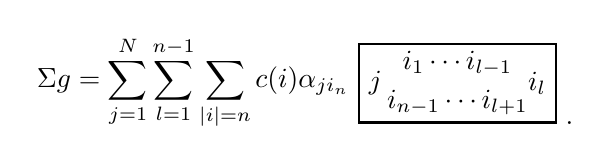
\begin{tikzpicture}[baseline]
	\node[left] at (0,0) {$\displaystyle\J\D\Sigma g=\sum_{j=1}^N \sum_{l=1}^{n-1}\sum_{|\ul{i}|=n} c(\ul{i}) \alpha_{ji_n}$};
	\draw[thick] (0,-.5) rectangle (2.5,.5);
	\node at (1.25,.25) {$i_1\cdots i_{l-1}$};
	\node at (1.25,-.25) {$i_{n-1}\cdots i_{l+1}$};
	\node[right] at (0,0) {$j$};
	\node[left] at (2.5,0) {$i_l$};
	\node[right] at (2.5,-.5) {.};
	\end{tikzpicture}
	\end{align*}

\begin{lem}
Let $g_1,\ldots, g_m\in \Pi\left(\mathscr{P}_{c.s.}\right)$. Set
	\begin{equation*}
		Q_m(g_1,\ldots,g_m)=\left[ (1\otimes\varphi)\circ\text{Tr}_A +(\varphi\otimes 1)\circ\text{Tr}_{A^{-1}}\right]\left( \J\D g_1\cdots \J\D g_m\right).
	\end{equation*}
Assume $R\geq4$, so that $\frac{2}{R}\leq\frac{1}{2}$. Then
	\begin{align*}
		\| Q_m(\Sigma g_1,\ldots, \Sigma g_m)\|_{R,\sigma} \leq \|A\|\frac{2^{m+1}}{R^{2m}} \prod_{u=1}^m \|g_u\|_{R,\sigma}.
	\end{align*}
In particular, $Q_m$ extends to a bounded multilinear operator on $\mathscr{P}^{(R,\sigma)}_{c.s.}$ with values in $\mathscr{P}^{(R,\sigma)}_{\varphi}$.
\end{lem}
\begin{proof}
First, for each $u=1,\ldots, m$  assume $g_u\in \pi_{n_u}(\mathscr{P}_{c.s.})$ and write $g_u=\sum_{|\ul{i}^{(u)}|=n_u} c_u(\ul{i}^{(u)}) X_{\ul{i}^{(u)}}$. By the computation preceding the statement of the lemma we can see that
	\begin{align*}
		\text{Tr}_{A^{-1}}( \J\D\Sigma g_1\cdots \J\D\Sigma g_m)=&\sum_{p_0,\ldots,p_m=1}^N [A^{-1}]_{p_mp_0}[\J\D\Sigma g_1]_{p_0p_1}\cdots [\J\D\Sigma g_m]_{p_{m-1}p_m}\\
			=&\sum_{j=1}^N \sum_{l_1=1}^{n_1-1}\cdots \sum_{l_m=1}^{n_m-1} \sum_{|\ul{i}^{(1)}|=n_1}\cdots \sum_{|\ul{i}^{(m)}|=n_m}\prod_{u=1}^m c_u(\ul{i}^{(u)}) \alpha_{i_{l_{u-1}}^{(u-1)}i_{n_u}^{(u)}}\\
			&\times
				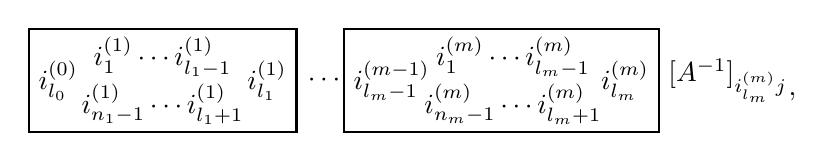
\begin{tikzpicture}[baseline]
				\draw[thick] (0,-.65) rectangle (3.4,.65);
				\node at (1.7,.3) {$i_1^{(1)}\cdots i_{l_1-1}^{(1)}$};
				\node at (1.7,-.3) {$i_{n_1-1}^{(1)}\cdots i_{l_1+1}^{(1)}$};
				\node[right] at (0,0) {$i_{l_0}^{(0)}$};
				\node[left] at (3.4,0) {$i_{l_1}^{(1)}$};
				\node at (3.75,0) {$\cdots$};
				\draw[thick] (4,-.65) rectangle (8,.65);
				\node at (6.15,.3) {$i_1^{(m)}\cdots i_{l_m-1}^{(m)}$};
				\node at (6.15,-.3) {$i_{n_m-1}^{(m)}\cdots i_{l_m+1}^{(m)}$};
				\node[right] at (4,0) {$i_{l_m-1}^{(m-1)}$};
				\node[left] at (8,0) {$i_{l_m}^{(m)}$};
				\node[right] at (8,0) {$[A^{-1}]_{i_{l_m}^{(m)} j}$};
				\node at (9.7,-.2) {,};
				\end{tikzpicture}
	\end{align*}
where $i_{l_0}^{(0)}=j$. Hence
	\begin{align*}
		(\varphi\otimes 1)\circ \text{Tr}_{A^{-1}}( \J\D\Sigma g_1\cdots \J\D\Sigma g_m)=&\sum_{j=1}^N \sum_{l_1,\ldots,l_m}\sum_{\ul{i}^{(1)},\ldots,\ul{i}^{(m)}} \prod_{u=1}^m c_u(\ul{i}^{(u)}) \alpha_{i_{l_{u-1}}^{(u-1)} i_{n_u}^{(u)}} \\
						&\times\varphi( X_{i_1^{(1)}}\cdots X_{i_{l_1-1}^{(1)}} \cdots X_{i_1^{(m)}}\cdots X_{i_{l_m-1}^{(m)}})\\
						&\times X_{i_{l_{m+1}}^{(m)}} \cdots X_{i_{n_m-1}^{(m)}} \cdots X_{i_{l_1+1}^{(1)}} \cdots X_{i_{n_1-1}^{(1)}}\cdot [A^{-1}]_{i_{l_m}^{(m)}j}.
	\end{align*}
Fix $l_1,\ldots, l_m$ in the above quantity, then the sum over $i_{l_0}^{(0)}$ and the multi-indices $\ul{i}^{(1)},\ldots,\ul{i}^{(m)}$ is a sum of monomials all with the same degree: $\sum_u n_u-l_u-1=:n_0$. By Lemma \ref{centralizer_commutes_with_A}, it suffices to bound $\|\rho^k(\cdot)\|_R$ for $k\in\{-n_0+1,\ldots, -1,0\}$. For $k=0$ we have
	\begin{align*}
		\left\| (\varphi\otimes 1)\circ\text{Tr}_{A^{-1}}\right.&\left.(\J\D\Sigma g_1\cdots \J\D\Sigma g_m)\right\|_R \\
				&\leq \sum_{j=1}^N \sum_{l_1,\ldots,l_m} \sum_{\ul{i}^{(1)},\ldots, \ul{i}^{(m)}} \prod_{u=1}^m \left|c_u\left(\ul{i}^{(u)}\right)\right| \left|[A^{-1}]_{i_m^{(m)} j}\right| R^{n_1-l_1-1+\cdots +n_m-l_m-1} 2^{l_1-1+\cdots +l_m-1}\\
				&\leq \sum_{l_1,\ldots,l_m} \sum_{\ul{i}^{(1)},\ldots, \ul{i}^{(m)}} \prod_{u=1}^m \left|c_u\left(\ul{i}^{(u)}\right)\right| \left\|A^{-1}\right\| R^{n_1+\cdots +n_m - 2m} \left(\frac{2}{R}\right)^{l_1+\cdots +l_m-m}\\
				&=\|A\| \prod_{u=1}^m \frac{1}{R^2}\| g_u\|_R \sum_{l_u=1}^{n_m-1} \left(\frac{2}{R}\right)^{l_u-1} \leq \|A\| \prod_{u=1}^m \frac{2}{R^2}\|g_u\|_R=\|A\| \prod_{u=1}^m \frac{2}{R^2}\|g_u\|_{R,\sigma},
	\end{align*}
where we have used $\|g_u\|_R=\|g_u\|_{R,\sigma}$.\par
Next, let $k\in\{ -n_0+1,\ldots, -1\}$ and suppose
	\begin{align*}
		\rho^k\left( X_{i_{l_{m}+1}^{(m)}}\right. &\cdots \left.X_{i_{n_m-1}^{(m)}}\cdots X_{i_{l_1+1}^{(1)}} \cdots X_{i_{n_1-1}^{(1)}}\right)\\
			&=X_{i_{a+1}^{(v)}}\cdots X_{i_{n_v-1}^{(v)}} \cdots X_{i_{l_1+1}^{(1)}} \cdots X_{i_{n_1-1}^{(1)}}\sigma_i\left( X_{i_{l_m+1}^{(m)}}\cdots X_{i_{n_m-1}^{(m)}} \cdots X_{i_{l_v+1}^{(v)}}\cdots X_{i_a^{(v)}}\right),
	\end{align*}
for some $v\in \{1,\ldots,m\}$ and some $a\in\{l_v+1,\ldots ,n_v-1\}$. The corresponding $\varphi$ output is
	\begin{align*}
		\varphi\left( X_{i_1^{(1)}}\right.& \left.\cdots X_{i_{l_1-1}^{(1)}}\cdots X_{i_1^{(m)}}\cdots X_{i_{l_m-1}^{(m)}}\right)\\
				&=\varphi\left( \sigma_i\left( X_{i_1^{(v)}}\cdots X_{i_{l_v -1}^{(v)}} \cdots X_{i_1^{(m)}}\cdots X_{i_{l_m-1}^{(m)}}\right) X_{i_1^{(1)}}\cdots X_{i_{l_1-1}^{(1)}} \cdots X_{i_1^{(v-1)}}\cdots X_{i_{l_{v-1}-1}^{(v-1)}}\right).
	\end{align*}
Using Lemma \ref{centralizer_commutes_with_A} we can in this case replace $\text{Tr}(A^{-1}\# \J\D\Sigma g_1\cdots \J\D\Sigma g_m)$ with
	\begin{equation*}
		\text{Tr}(\J\D\Sigma g_1 \cdots \J\D\Sigma g_v\#A^{-1}\#(\sigma_{-i}\otimes\sigma_{-i})(\J\D\Sigma g_{v+1}\cdots \J\D\Sigma g_m))
	\end{equation*}
so that output of $\rho^k$ changes to
	\begin{align*}
		X_{i_{a+1}^{(v)}}\cdots X_{i_{n_v-1}^{(v)}} \cdots X_{i_{l_1+1}^{(1)}} \cdots X_{i_{n_1-1}^{(1)}} X_{i_{l_m+1}^{(m)}}\cdots X_{i_{n_m-1}^{(m)}} \cdots \sigma_i\left(X_{i_{l_v+1}^{(v)}}\cdots X_{i_a^{(v)}}\right),
	\end{align*}
and the output of $\varphi$ changes to
	\begin{align*}
		\varphi\left( \sigma_i\left( X_{i_1^{(v)}}\cdots X_{i_{l_v -1}^{(v)}}\right) \cdots X_{i_1^{(m)}}\cdots X_{i_{l_m-1}^{(m)}} X_{i_1^{(1)}}\cdots X_{i_{l_1-1}^{(1)}} \cdots X_{i_1^{(v-1)}}\cdots X_{i_{l_{v-1}-1}^{(v-1)}}\right).
	\end{align*}
Hence it suffices to consider when $v=m$. In this case we further fix $\ul{i}^{(1)},\ldots, \ul{i}^{(m-1)}$ and denote $F_u:=X_{i_1^{(u)}}\cdots X_{i_{l_u-1}^{(u)}}$ and $G_u:=X_{i_{l_u+1}^{(u)}}\cdots X_{i_{n_u-1}^{(u)}}$. Consider
	\begin{align*}
		\sum_{j=1}^N &\sum_{\ul{i}^{(m)}}  c_m\left(\ul{i}^{(m)}\right) \alpha_{i_{l_{m-1}}^{(m-1)} i_{n_m}^{(m)}}[A^{-1}]_{i_{l_m}^{(m)} j}\\
				&\times \varphi\left( \sigma_i\left( X_{i_1^{(m)}}\cdots X_{i_{l_m -1}^{(m)}}\right)  F_1\cdots F_{m-1}\right)   X_{i_{a+1}^{(m)}}\cdots X_{i_{n_m-1}^{(m)}}G_1\cdots G_{m-1} \sigma_i\left(X_{i_{l_m+1}^{(m)}}\cdots X_{i_a^{(m)}}\right)\\
		=&\sum_{j=1}^N \sum_{\ul{i}^{(m)}}\ \sum_{\hat{i}_1^{(m)},\ldots, \hat{i}_{l_m-1}^{(m)}=1}^N\  \sum_{\hat{i}_{l_m+1}^{(m)},\ldots, \hat{i}_a^{(m)}=1}^N c_m\left(\ul{i}^{(m)}\right) \alpha_{i_{l_{m-1}}^{(m-1)} i_{n_m}^{(m)}}\prod_{t\neq l_m}[A^{-1}]_{i_t^{(m)} \hat{i}_t^{(m)}} \cdot [A^{-1} ]_{i_{l_m}^{(m)} j}\\
				&\times \varphi\left( X_{\hat{i}_1^{(m)}}\cdots X_{\hat{i}_{l_m-1}^{(m)}}F_1\cdots F_{m-1}\right)  X_{i_{a+1}^{(m)}}\cdots X_{i_{n_m-1}^{(m)}}G_1\cdots G_{m-1} X_{\hat{i}_{l_m+1}^{(m)}}\cdots X_{\hat{i}_a^{(m)}}\\
		=&\sum_{\ul{i}^{(m)}} \sum_{|\ul{\hat{i}}^{(m)}|=a} c_m\left( \ul{i}^{(m)}\right) \alpha_{i_{l_{m-1}}^{(m-1)} i_{n_m}^{(m)}}\prod_{t=1}^a [A^{-1}]_{i_t^{(m)} \hat{i}_t^{(m)}} \varphi\left( X_{\hat{i}_1^{(m)}}\cdots X_{\hat{i}_{l_m-1}^{(m)}}F_1\cdots F_{m-1}\right) \\
				&\times X_{i_{a+1}^{(m)}}\cdots X_{i_{n_m-1}^{(m)}}G_1\cdots G_{m-1} X_{\hat{i}_{l_m+1}^{(m)}}\cdots X_{\hat{i}_a^{(m)}}\\
		=&\sum_{\ul{j}^{(m)}} c_m\left( \ul{j}^{(m)}\right) \alpha_{i_{l_{m-1}}^{(m-1)} j_{n_m-a}^{(m)}}\varphi\left( X_{j_{n_m-a+1}^{(m)}}\cdots X_{i_{n_m-a+l_m-1}^{(m)}} F_1\cdots F_{m-1}\right)\\
			&\times  X_{j_1^{(m)}} \cdots X_{j_{n_m-a-1}^{(m)}} G_1\cdots G_{m-1} X_{i_{n_m-a+l_m+1}^{(m)}} \cdots X_{j_{n_m}^{(m)}},
	\end{align*}
where in the final equality we have used the characterization of the coefficients of elements of $\mathscr{P}_{c.s.}$ given by (\ref{cyclically_symmetric_coefficients_negative}). We note that while the multi-index has changed to $\ul{j}^{(m)}$, there are still $l_m-1$ terms inside $\varphi$ and $n_m-l_m-1$ outside. Thus we have
	\begin{align*}
		\left\| \rho^k\circ(\varphi\otimes 1)\circ\right.&\left.\text{Tr}_{A^{-1}}(\J\D\Sigma g_1\cdots \J\D\Sigma g_m)\right\|_R \\
				&\leq \sum_{l_1,\ldots,l_m} \sum_{\ul{i}^{(1)},\ldots, \ul{i}^{(m)}} \prod_{u=1}^m \left| c_u\left(\ul{i}^{(u)}\right)\right| R^{n_1-l_1-1+\cdots +n_m-l_m-1}2^{l_1-1+\cdots +l_m-1}\\
				&=\sum_{l_1,\ldots,l_m} \sum_{\ul{i}^{(1)},\ldots, \ul{i}^{(m)}} \prod_{u=1}^m \left| c_u\left(\ul{i}^{(u)}\right)\right| R^{n_1+\cdots +n_m - 2m}\left(\frac{2}{R}\right)^{l_1-1+\cdots +l_m-1}\\
				&=\prod_{u=1}^m \frac{1}{R^2} \|g_u\|_{R} \sum_{l_u=1}^{n_u-1} \left(\frac{2}{R}\right)^{l_u-1}\leq \prod_{u=1}^m \frac{2}{R^2} \|g_u\|_{R,\sigma}\leq \|A\| \prod_{u=1}^m \frac{2}{R^2} \|g_u\|_{R,\sigma}.
	\end{align*}
Thus	
	\begin{align*}
		\left\| (\varphi\otimes 1)\circ\text{Tr}_{A^{-1}}(\J\D\Sigma g_1\cdots \J\D\Sigma g_m)\right\|_{R,\sigma}\leq \|A\| \frac{2^m}{R^{2m}}\prod_{u=1}^m \|g_u\|_{R,\sigma},
	\end{align*}
and similar estimates show
	\begin{align*}
		\left\| (\varphi\otimes 1)\circ\text{Tr}_{A}(\J\D\Sigma g_1\cdots \J\D\Sigma g_m)\right\|_{R,\sigma}\leq \|A\| \frac{2^m}{R^{2m}}\prod_{u=1}^m \|g_u\|_{R,\sigma}.
	\end{align*}\par
Now let $g_1,\ldots, g_m\in \mathscr{P}_{c.s.}$ be arbitrary. We note that $\pi_{n_u}(g_u)\in\mathscr{P}_{c.s.}$ for each $n_u\geq 0$ since $[\rho,\pi_{n_u}]=0$. Then since $Q_m$ is multi-linear we have
	\begin{align*}
		Q_m(\Sigma g_1,\ldots,\Sigma g_m)= \sum_{n_1,\ldots, n_m=0}^\infty Q_m\left(\Sigma \pi_{n_1}(g_1),\ldots, \Sigma \pi_{n_m}(g_m)\right),
	\end{align*}
and hence
	\begin{align*}
		\left\| Q_m(\Sigma g_1,\ldots,\Sigma g_m)\right\|_{R,\sigma} &\leq \sum_{n_1,\ldots, n_m} \|A\|\frac{2^{m+1}}{R^{2m}} \prod_{u=1}^m \|\pi_{n_u}(g_u)\|_{R,\sigma} \\
				&= \|A\| \frac{2^{m+1}}{R^{2m}} \prod_{u=1}^m \sum_{n_u=0}^\infty \|\pi_{n_u}(g_u)\|_{R,\sigma}=\|A\|\frac{2^{m+1}}{R^{2m}} \prod_{u=1}^m \|g_u\|_{R,\sigma}.
	\end{align*}
Thus $Q_m$ extends to a bounded multilinear operator on $\mathscr{P}^{(R,\sigma)}_{c.s.}$. That $Q_m$ takes values in $\mathscr{P}^{(R,\sigma)}_\varphi$ follows from Lemma \ref{centralizer_commutes_with_A}.
\end{proof}

\begin{lem}\label{Q_m}
For $f,g\in \mathscr{P}_{c.s.}^{(R,\sigma)}$ set $Q_m(\Sigma g)=Q_m(\Sigma g,\ldots, \Sigma g)$ and assume $R\geq4$. Then
	\begin{align*}
		\left\| Q_m(\Sigma g)- Q_m(\Sigma f)\right\|_{R,\sigma} \leq \|A\|\frac{2^{m+1}}{R^{2m}} \sum_{k=0}^{m-1} \|g\|_{R,\sigma}^k \|f\|_{R,\sigma}^{m-k-1} \|f-g\|_{R,\sigma}.
	\end{align*}
In particular, $\|Q_m(\Sigma g)\|_{R,\sigma}\leq \|A\| \frac{2^{m+1}}{R^{2m}} \|g\|_{R,\sigma}^m$.
\end{lem}
\begin{proof}
Using a telescoping sum we have
	\begin{align*}
		\|Q_m(\Sigma f)&-Q_m(\Sigma g)\|_{R,\sigma}\\
			&=\left\| \sum_{k=0}^{m-1} Q_m(\underbrace{\Sigma g,\ldots,\Sigma g}_k,\underbrace{\Sigma f,\ldots,\Sigma f}_{m-k})-Q_m(\underbrace{\Sigma g,\ldots,\Sigma g}_{k+1},\underbrace{\Sigma f,\ldots,\Sigma f}_{m-k-1})\right\|_{R,\sigma}\\
					&\leq \sum_{k=0}^{m-1} \| Q_m(\underbrace{\Sigma g,\ldots \Sigma g}_{k},\Sigma f-\Sigma g,\underbrace{\Sigma f,\ldots,\Sigma f}_{m-k-1})\|_{R,\sigma}\\
					&\leq  \|A\| \frac{2^{m+1}}{R^{2m}} \sum_{k=0}^{m-1}\|g\|_{R,\sigma}^k\|f\|_{R,\sigma}^{m-k-1}\|f-g\|_{R,\sigma}.
	\end{align*}
\end{proof}

\begin{lem}\label{Q_2}
Assume $R\geq4$. Let $g\in\mathscr{P}^{(R,\sigma)}_{c.s.}$ be such that $\|g\|_{R,\sigma}<\frac{R^2}{2}$, and set
	\begin{equation*}
		Q(\Sigma g)=\sum_{m\geq 0} \frac{(-1)^m}{m+2}Q_{m+2}(\Sigma g).
	\end{equation*}
Then this series converges in $\|\cdot\|_{R,\sigma}$. Moreover, in the sense of analytic functional calculus on $M_{N}(W^*(\mathscr{P}\otimes \mathscr{P}^{op},\varphi\otimes\varphi^{op}))$, we have the equality
	\begin{equation*}
		Q(\Sigma g)=\left[ (1\otimes\varphi)\circ\text{Tr}_{A}+(\varphi\otimes 1)\circ\text{Tr}_{A^{-1}} \right] \left\{ \J\D \Sigma g - \log(1+\J\D\Sigma g)\right\}.
	\end{equation*}
Furthermore, the function $Q$ satisfies the local Lipschitz condition on $\left\{g\in\mathscr{P}^{(R,\sigma)}_{c.s.}\colon \|g\|_{R,\sigma} < R^2/2\right\}$
	\begin{align*}
		\left\| Q(\Sigma g)-Q(\Sigma f)\right\|_{R,\sigma} \leq \| f-g\|_{R,\sigma} \frac{2\|A\|}{R^2} \left( \frac{1}{\left(1-\frac{2\|f\|_{R,\sigma}}{R^2}\right)\left(1-\frac{2\|g\|_{R,\sigma}}{R^2}\right)} - 1\right),
	\end{align*}
and the bound
	\begin{align*}
		\|Q(\Sigma g)\|_{R,\sigma} \leq \frac{ 4\|A\| \|g\|_{R,\sigma}^2}{R^4-2R^2 \|g\|_{R,\sigma}}.
	\end{align*}
\end{lem}
\begin{proof}
Let $\kappa=R^2/2$ and $\lambda = \|g\|_{R,\sigma}$. From Lemma \ref{Q_m} we know $\|Q_{m+2}(\Sigma g)\|_{R,\sigma} \leq  2\|A\| \left(\frac{\lambda}{\kappa}\right)^{m+2}$. Since $\lambda<\kappa$, the series defining $Q$ converges. The functional calculus equality then follows from $\log(1+x)=-\sum_{m\geq 1} \frac{(-x)^m}{m}$. Finally, since $m+2\geq 2$ in our series we obtain
	\begin{align*}
		\| Q(\Sigma g) - Q(\Sigma f)\|_{R,\sigma} &\leq \sum_{m\geq 0} \frac{1}{m+2} \| Q_{m+2}(\Sigma g) - Q_{m+2}(\Sigma f)\|_{R,\sigma}\\
								&\leq \|f-g\|_{R,\sigma} \|A\| \sum_{m\geq 0} \sum_{k=0}^{m+1} \kappa^{-m-2}\|f\|_{R,\sigma}^{m-k+1}\|g\|_{R,\sigma}^k\\
								&\leq \|f -g\|_{R,\sigma} \frac{\|A\| }{\kappa} \left( \sum_{l\geq 0}\sum_{k\geq 0} \kappa^{-l}\|f\|_{R,\sigma}^l \kappa^{-k} \|g\|_{R,\sigma}^k - 1\right),
	\end{align*}
where we have written $m=l+k-1$ which is non-negative so long as $l$ and $k$ are not both zero. Using $\|f\|_{R,\sigma}, \|g\|_{R,\sigma} < \kappa$ we see that
	\begin{align*}
		\| Q(\Sigma g) - Q(\Sigma f)\|_{R,\sigma} \leq \| f- g\|_{R,\sigma} \frac{2\|A\|}{R^2}\left( \frac{1}{\left(1-\frac{2\|f\|_{R,\sigma}}{R^2}\right)\left(1-\frac{2\|g\|_{R,\sigma}}{R^2}\right)} - 1\right).
	\end{align*}
Setting $f=0$ yields the bound
	\begin{align*}
		\|Q(\Sigma g)\|_{R,\sigma}\leq \|g\|_{R,\sigma} \frac{2\|A\|}{R^2} \frac{2\|g\|_{R,\sigma}}{R^2-2\|g\|_{R,\sigma}} = \frac{ 4\|A\| \|g\|_{R,\sigma}^2}{R^4-2R^2 \|g\|_{R,\sigma}},
	\end{align*}
as claimed.
\end{proof}

The proof of the following lemma is purely computational and left to the reader.

\begin{lem}
If $f=\D g$ for $g\in \mathscr{P}_\varphi^{(R,\sigma)}$ then 
	\begin{align}\label{eigenvalue_f}
		A^{-1}\# \sigma_{-i}(f)=f.
	\end{align}
Moreover, if $g=g^*$ then
	\begin{align}\label{dot_product_to_vector_product}
		\D\left( \frac{1}{2}\J_\sigma X^{-1}\# f\# f\right)=\J_\sigma f\# \J_\sigma X^{-1}\# f=\J f\# f.
	\end{align}
\end{lem}

\begin{lem}\label{dot_product_in_centralizer}
Suppose $f^{(i)}=\D\Sigma g_i$ with $g_i\in \mathscr{P}_{c.s.}$ for $i=1,2$. Then $(1+A)\# f^{(1)}\# f^{(2)}\in\mathscr{P}_\varphi$. Furthermore,
	\begin{align*}
		\left\|(1+A)\# f^{(1)}\# f^{(2)} \right\|_{R,\sigma} \leq \frac{2N\|A\|}{R^2} \|g_1\|_{R,\sigma}\|g_2\|_{R,\sigma}.
	\end{align*}
\end{lem}
\begin{proof}
From (\ref{eigenvalue_f}) it is easy to see that $(1+A)\# f^{(1)}\# f^{(2)}\in\mathscr{P}_\varphi$. Now, write $g_1=\sum_{m=1}^\infty \sum_{|\ul{i}|=m} c_1(\ul{i}) X_{\ul{i}}$ and $g_2 = \sum_{n=1}^\infty \sum_{|\ul{j}|=n}c_2(\ul{j})X_{\ul{j}}$. Then (\ref{cyclic_derivative_of_cyclically_symmetric}) implies
	\begin{align*}
		f_j^{(1)}=\sum_{m=1}^\infty \sum_{\substack{|\ul{i}|=m-1\\ a\in\{1,\ldots, N\}}}\alpha_{ja} c_1(\ul{i}\cdot a) X_{\ul{i}}\qquad\text{ and }\qquad f_i^{(2)} = \sum_{n=1}^\infty \sum_{\substack{|\ul{j}|=n-1\\ b\in\{1,\ldots, N\}}} \alpha_{ib} c_2(\ul{j}\cdot b) X_{\ul{j}}.
	\end{align*}
Hence
	\begin{align*}
		(1+A)\# f^{(1)}\# f^{(2)} =\sum_{m,n=1}^\infty \sum_{i,j=1}^N [1+A]_{ij}  \sum_{a,b=1}^N \sum_{\substack{|\ul{i}|=m-1\\ |\ul{j}|=n-1}} \alpha_{ja}\alpha_{ib} c_1(\ul{i}\cdot a)c_2(\ul{j}\cdot b) X_{\ul{i}} X_{\ul{j}}.
	\end{align*}
It suffices to bound $\|\rho^k(\cdot )\|_R$ for $k\in\{-m-n+1,\ldots, 0\}$. First, for $k=0$ we simply have
	\begin{align*}
		\| (1+A)\#f^{(1)}\# f^{(2)}\|_R &\leq \sum_{i,j=1}^N | [1+A]_{ij}| \sum_{m,n=1}^\infty \sum_{\substack{|\ul{i}|=m-1,a\\ |\ul{j}|=n-1, b}} |c_1\left(\ul{i}\cdot a\right) c_2\left(\ul{j}\cdot b\right)| R^{m+n-2}\\
							&\leq N(1+\|A\|)\frac{1}{R^2} \left(\sum_{m=1}^\infty\sum_{\ul{i},a} |c_1(\ul{i}\cdot a)| R^m\right)\left(\sum_{n=1}^\infty \sum_{\ul{j},b} |c_2(\ul{j}\cdot b) R^n\right)\\
							&\leq \frac{2N\|A\|}{R^2}\|g_1\|_{R,\sigma}\|g_2\|_{R,\sigma}.
	\end{align*}
For $-m+1\leq k\leq -1$, we further fix $i,j,a,b$. Then using (\ref{cyclically_symmetric_coefficients_negative}) we have
	\begin{align*}
		\sum_{\substack{|\ul{i}|=m-1\\ |\ul{j}|=n-1}}  c_1(\ul{i}\cdot a)c_2(\ul{j}\cdot b)\rho^k\left( X_{\ul{i}} X_{\ul{j}}\right)=\sum_{\substack{ |\ul{\hat{l}}|=k\\ |\ul{i}|=m-k-1\\ |\ul{j}=n-1}}  c_2(\ul{j}\cdot b) c_1\left(\ul{i}\cdot a\cdot\ul{\hat{l}}\right) X_{\ul{j}} X_{\ul{\hat{l}}}.
	\end{align*}
Thus
	\begin{align*}
		\sum_{m,n=1}^\infty &\left\| \sum_{i,j=1}^N [1+A]_{ij}  \sum_{a,b=1}^N \sum_{\substack{|\ul{i}|=m-1\\ |\ul{j}|=n-1}} \alpha_{ja}\alpha_{ib} c_1(\ul{i}\cdot a)c_2(\ul{j}\cdot b)\rho^k\left( X_{\ul{i}} X_{\ul{j}}\right)\right\|_R\\
				 &\leq \sum_{m,n=1}^\infty \sum_{i,j=1}^N |[1+A]_{ij}| \sum_{\substack{ |\ul{i}|=m\\ |\ul{j}|=n}} |c_1(\ul{i}) c_2(\ul{j}) | R^{n+m-2}\\
				 &\leq N(1+\|A\|) \frac{1}{R^2}\left(\sum_{m=1}^\infty\sum_{\ul{i},a} |c_1(\ul{i}\cdot a)| R^m\right)\left(\sum_{n=1}^\infty \sum_{\ul{j},b} |c_2(\ul{j}\cdot b) R^n\right)\\
							&\leq \frac{2N\|A\|}{R^2}\|g_1\|_{R,\sigma}\|g_2\|_{R,\sigma}.
	\end{align*}
The cases for $-m-n+1\leq k \leq -m$ are similar after using $\sigma_i(g_1)=g_1$. Thus the claimed bound holds.
\end{proof}















\begin{lem}\label{W_patchwork}
Assume $R\geq 4$. If $f=\D\Sigma g$ for $g\in \P_{c.s.}^{(R,\sigma)}$ with $\|g\|_{R,\sigma}\leq S$ and $W\in \P_{c.s.}^{(S,\sigma)}$, then $W(f)\in \P_\varphi^{(R,\sigma)}$ with
	\begin{align*}
		\| W(f)\|_{R,\sigma} \leq \frac{N(1+\|A\|)}{8} \|W\|_{S,\sigma}.
	\end{align*}
Furthermore, if $f^{(j)}=\D\Sigma g_j$ for $g_j\in \P_{c.s.}^{(R,\sigma)}$ with $\|g_j\|_{R,\sigma}\leq S$, $j\in\{1,2\}$, then
	\begin{align*}
		\|W(f^{(1)}) - W(f^{(2)})\|_{R,\sigma} \leq \frac{N(1+\|A\|)}{8} \sum_{j=1}^N \|\delta_j(W)\|_{S\otimes_\pi S} \|g_1 - g_2\|_{R,\sigma}.
	\end{align*}
\end{lem}
\begin{proof}
We will first show that for each $j,k\in\{1,\ldots, N\}$, $n\geq 1$, and $0\leq s\leq n-1$ we have
	\begin{align*}
		\left\|\sum_{j=1}^N (1\otimes[\sigma_{-i}\circ\pi_s])\circ\delta_j(\pi_n(f_k))\# X_j\right\|_R \leq \frac{N(1+\|A\|)}{8}\|\pi_{n+1}(g)\|_{R,\sigma}.
	\end{align*}
Note that $\pi_n(f)=\D\Sigma \pi_{n+1}(g)$ and so we observe that Lemma \ref{change_of_variables}.(iii) implies
	\begin{align*}
		(1\otimes\sigma_{-i})\circ\delta_j(\pi_n(f_k)) &= \sum_{\ell=1}^N \left[\frac{1+A}{2}\right]_{j\ell} (1\otimes\sigma_{-i})\circ \bar{\partial}_\ell(\pi_n(f_k))\\
			&= \sum_{\ell=1}^N \left[\frac{1+A}{2}\right]_{j\ell} \partial_k(\pi_n(f_\ell)^*)^\diamond.
	\end{align*}
(Lemma \ref{change_of_variables}.(iii) was only proved for $Y=\D G$ with $G$ self-adjoint, but it is clear that the same argument for a non-self-adjoint element yields $(\J_\sigma \D G)^* = (\otimes\otimes 1)(\J_\sigma \D (G^*))$). Now, suppose for each $\ell\in\{1,\ldots,N\}$
	\begin{align*}
		\pi_n(f_\ell)^* = \sum_{|\ul{i}|=n} c_\ell(\ul{i}) X_{\ul{i}},\qquad c_\ell(\ul{i})\in \C.
	\end{align*}
Then
	\begin{align*}
		\sum_{j=1}^N &(1\otimes[\sigma_{-i}\circ\pi_s])\circ\delta_j(\pi_n(f_k))\# X_j = \sum_{j=1}^N (1\otimes\pi_s)\left( (1\otimes\sigma_{-i})\circ\delta_j(\pi_n(f_k))\right) \# X_j\\
			&=\sum_{j,\ell=1}^N \left[\frac{1+A}{2}\right]_{j\ell} (1\otimes \pi_s)\left( \partial_k(\pi_n(f_\ell)^*)^\diamond\right)\# X_j\\
			&=\sum_{j,\ell=1}^N \left[\frac{1+A}{2}\right]_{j\ell}\sum_{n\geq 0} \sum_{|\ul{i}|=n} c_\ell(\ul{i}) \left[ \left[\frac{2}{1+A}\right]_{i_{s+1}k}X_{i_1}\cdots X_{i_s}\otimes X_{i_{s+2}}\cdots X_{i_n}\right]^\diamond\# X_j\\
			&=\sum_{\ell=1}^N \sum_{n\geq 0} \sum_{|\ul{i}|=n} c_\ell(\ul{i}) \left[\frac{2}{1+A}\right]_{i_{s+1}k}X_{i_{s+2}}\cdots X_{i_n}\left(\frac{X_\ell+[AX]_{\ell}}{2}\right)X{i_1}\cdots X_{i_s}.
	\end{align*}
Recall that $\left|\left[\frac{2}{1+A}\right]_{i_{s+1}k}\right|\leq 1$ and $\|[AX]_\ell\|_R\leq \|A\| R$. We then have
	\begin{align*}
		\left\|\sum_{j=1}^N (1\otimes[\sigma_{-i}\circ\pi_s])\circ\delta_j(\pi_n(f_k))\# X_j\right\|_R &\leq \sum_{\ell=1}^N \sum_{n\geq 0} \sum_{|\ul{i}|=n} |c_\ell(\ul{i})| R^{n-s-1}\left(\frac{1+\|A\|}{2} R\right)R^s\\
			&=\sum_{\ell=1}^N \frac{1+\|A\|}{2} \|\pi_n(f_\ell)\|_R =\sum_{\ell=1}^N \frac{1+\|A\|}{2} \|\D_\ell \Sigma \pi_{n+1}(g)\|_R\\
			&= \frac{N(1+\|A\|)}{2R} \|\pi_{n+1}(g)\|_{R,\sigma} \leq \frac{N(1+\|A\|)}{8}\|\pi_{n+1}(g)\|_{R,\sigma},
	\end{align*}
where we have used Lemma \ref{cyclic_derivative_bounded} in the second to last step.

Now, suppose for some $n\in\N$
	\begin{align*}
		W = \sum_{|\ul{i}|=n} b(\ul{i}) X_{\ul{i}} \in \P_{c.s.},
	\end{align*}
for $b(\ul{i})\in \C$. Then by (\ref{cyclically_symmetric_coefficients_positive}) we have
	\begin{align*}
		b(\ul{i}\cdot \ul{j}) = \sum_{|\ul{k}|=|\ul{i}|} b(\ul{j}\cdot \ul{k}) A(\ul{k},\ul{i}).
	\end{align*}
Since $f=\D\Sigma g$, we know from (\ref{eigenvalue_f}) that $\sigma_{-i}(\pi_{k_j}(f)) = \pi_{k_j}( [A\# f]_{i_j})$ and hence $W(f)\in \P_\varphi^{(R)}$:
	\begin{align*}
		\sigma_{-i}(W(f)) &= \sum_{|\ul{i}|=n} b(\ul{i}) \sigma_{-i}(f_{i_1})\cdots \sigma_{-i}(f_{i_n})\\
					&=\sum_{|\ul{i}|=n} \sum_{|\ul{j}|=n} b(\ul{i}) A(\ul{i},\ul{j}) f_{\ul{j}}= \sum_{|\ul{j}|=n} b(\ul{j}) f_{\ul{j}} = W(f).
	\end{align*}
Thus
	\begin{align*}
		\| W(f)\|_{R,\sigma} = \sum_{M\geq 0} \max_{0\leq t\leq M-1} \|\rho^t(\pi_M(W(f)))\|_R.
	\end{align*}
Fix $M\geq 1$ and $0\leq t\leq M-1$. We have
	\begin{align*}
		\rho^t(\pi_M(W(f))) = \sum_{|\ul{i}|=n} \sum_{k_1+\cdots + k_n = M} b(\ul{i})\rho^t( \pi_{k_1}(f_{i_1})\cdots \pi_{k_n}(f_{i_n})).
	\end{align*}
For fixed $k_1,\ldots, k_n$ there exists $a\in\{1,\ldots, n\}$ such that
	\begin{align*}
		k_{a+1}+\cdots +k_n \leq t < k_a+\cdots +k_n,\qquad	\text{ or }\qquad	0 \leq \underbrace{t- (k_{a+1}+\cdots+k_n)}_{=:s} < k_a.
	\end{align*}
Since $f=\D\Sigma g$, we know from (\ref{eigenvalue_f}) that $\sigma_{-i}(\pi_{k_j}(f)) = \pi_{k_j}( [A\# f]_{i_j})$. Hence we have
	\begin{align*}
		\sum_{|\ul{i}|=n} &b(\ul{i})\rho^t( \pi_{k_1}(f_{i_1})\cdots \pi_{k_n}(f_{i_n}))\\
		 &=\sum_{\substack{|\ul{i}|=a\\ |\ul{j}|=n-a}}b(\ul{i}\cdot \ul{j}) \rho^t( \pi_{k_1}(f_{i_1})\cdots \pi_{k_n}(f_{i_n})) \\
		 &= \sum_{\substack{|\ul{i}|=a\\ |\ul{j}|=n-a}} b(\ul{i}\cdot \ul{j}) \rho^s\left( \sum_{|\ul{\ell}|=|\ul{j}|} A(\ul{j},\ul{\ell}) \pi_{k_{a+1}}(f_{\ell_1})\cdots \pi_{k_n}(f_{\ell_{n-a}}) \pi_{k_1}(f_{i_1})\cdots \pi_{k_a}(f_{i_a})\right) \\
		 &= \sum_{\substack{|\ul{i}|=a\\ |\ul{\ell}|=n-a}} b(\ul{\ell}\cdot \ul{i}) \rho^s\left(\pi_{k_{a+1}}(f_{\ell_1})\cdots \pi_{k_n}(f_{\ell_{n-a}}) \pi_{k_1}(f_{i_1})\cdots \pi_{k_a}(f_{i_a})\right).
	\end{align*}
Since $\|\cdot\|_R$ is invariant under cyclic rotations (provided there is a consistent degree rotated), we can instead consider the above after $\ell$ rotations which we note is
	\begin{align*}
		\sum_{\substack{|\ul{i}|=a\\ |\ul{\ell}|=n-a}} b(\ul{\ell}\cdot \ul{i})\pi_{k_1}(f_{i_1})\cdots \pi_{k_a}(f_{i_a}) \left( \sum_{j=1}^N (1\otimes[\sigma_{-i}\circ\pi_s])\circ\delta_j(\pi_{k_a}(f_{i_a}))\# X_j\right)\pi_{k_{a+1}}(f_{\ell_1}) \cdots \pi_{k_n}(f_{\ell_{n-a}}).
	\end{align*}
So the inequality from the first part of the proof implies
	\begin{align*}
		\|\rho^t(\pi_M(W(f)))\|_R &\leq \sum_{k_1+\cdots +k_n=M}\sum_{\substack{|\ul{i}|=a\\ |\ul{\ell}|=n-a}} |b(\ul{\ell}\cdot \ul{i})| \frac{N(1+\|A\|)}{8} \| \pi_{k_1+1}(g)\|_{R,\sigma}\cdots \|\pi_{k_n+1}(g)\|_{R,\sigma}\\
			& \leq \frac{N(1+\|A\|)}{8}\sum_{|\ul{i}|=n} |b(\ul{i})| \sum_{k_1+\cdots +k_n=M}\| \pi_{k_1+1}(g)\|_{R,\sigma}\cdots \|\pi_{k_n+1}(g)\|_{R,\sigma},
	\end{align*}
and hence
	\begin{align*}
		\|W(f)\|_{R,\sigma} &\leq \frac{N(1+\|A\|)}{8}\sum_{|\ul{i}|=n} |b(\ul{i})| \sum_{M\geq 0}\sum_{k_1+\cdots +k_n=M}\| \pi_{k_1+1}(g)\|_{R,\sigma}\cdots \|\pi_{k_n+1}(g)\|_{R,\sigma}\\
			&\leq \frac{N(1+\|A\|)}{8}\sum_{|\ul{i}|=n} |b(\ul{i})| \|g\|_{R,\sigma}^n \leq \frac{N(1+\|A\|)}{8}\|W\|_S=\frac{N(1+\|A\|)}{8}\|W\|_{S,\sigma}.
	\end{align*}
Then for more general $W$ of the form
	\begin{align*}
		W=\sum_{n\geq 0} \sum_{|\ul{i}|=n} b(\ul{i}) X_{\ul{i}}
	\end{align*}
we simpy have
	\begin{align*}
		\|W(f)\|_{R,\sigma} \leq \sum_{n\geq 0} \| \pi_n(W)(f)\|_{R,\sigma} \leq \sum_{n\geq 0} \frac{N(1+\|A\|)}{8} \|\pi_n(W)\|_{S,\sigma} = \frac{N(1+\|A\|)}{8} \|W\|_{S,\sigma}.
	\end{align*}

Finally, if $f^{(j)}=\D\Sigma g_j$ for $g_j\in \P_{c.s.}^{(R,\sigma)}$ with $\|g_j\|_R\leq S$, $j\in\{1,2\}$, and $W$ is of the form
	\begin{align*}
		W=\sum_{n\geq 0} \sum_{|\ul{i}|=n} b(\ul{i}) X_{\ul{i}},
	\end{align*}
we have
	\begin{align*}
		W(f^{(1)})-W(f^{(2)}) &= \sum_{n\geq 0}\sum_{|\ul{i}|=n} b(\ul{i}) \left( f^{(1)}_{\ul{i}} - f^{(2)}_{\ul{i}}\right)\\
			&= \sum_{n\geq 0}\sum_{|\ul{i}|=n} b(\ul{i}) \sum_{j=1}^n \left[\delta_j(X_{\ul{i}})(f^{(1)},f^{(2)})\right]\# (f^{(1)}_j - f^{(2)}_j),
	\end{align*}
where $\delta_j(X_{\ul{i}}(f^{(1)},f^{(2)})$ means the $X_j$ to the left of the `$\otimes$' are evaluated at $X=f^{(1)}$ and the $X_j$ to the right are evaluated at $X=f^{(2)}$. Then the same estimates as above yields
	\begin{align*}
		\| W(f^{(1)}) - W(f^{(2)}) \|_{R,\sigma} &\leq \frac{N(1+\|A\|)}{8}\sum_{j=1}^N \sum_{n\geq 0} |b(\ul{i})| S^{n-1} \| g_1 - g_2\|_{R,\sigma}\\
			&\leq \frac{N(1+\|A\|)}{8}\sum_{j=1}^N \|\delta_j(W)\|_{S\otimes_\pi S} \|g_1 - g_2\|_{R,\sigma}.
	\end{align*}
\end{proof}



\begin{cor}\label{F}
Assume $R\geq4$. Let $g\in \mathscr{P}^{(R,\sigma)}_{c.s.}$ and assume that $\|g\|_{R,\sigma}< \frac{R^2}{2}$. Let $S\geq R+\frac{R^2}{2}$ and let $W\in \mathscr{P}^{(S)}_{c.s.}$. Let
	\begin{align*}
		F(g) =& - W(X+\D\Sigma g) -   \frac{1}{4}\left\{(1+A)\#\D\Sigma g\right\} \#\D\Sigma g\\
			& + \left[(1\otimes\varphi)\circ\text{Tr}_{A}+(\varphi\otimes 1)\circ\text{Tr}_{A^{-1}}\right]\circ\log(1+\J\D\Sigma g)\\
			=& - W(X+\D\Sigma g) -   \frac{1}{4}\left\{(1+A)\#\D\Sigma g\right\} \#\D\Sigma g \\
			 &+  \left[(1\otimes\varphi)\circ\text{Tr}_{A}+(\varphi\otimes 1)\circ\text{Tr}_{A^{-1}}\right](\J\D\Sigma g)-Q(\Sigma g).
	\end{align*}
Then $F(g)$ is a well-defined function from $\mathscr{P}^{(R,\sigma)}_{c.s.}$ to $\mathscr{P}^{(R,\sigma)}_{\varphi}$. Moreover, $g\mapsto F(g)$ is locally Lipschitz on $\{g\colon \|g\|_{R,\sigma}< R^2/2\}$:
	\begin{align*}
		\| F(g)-F(f)\|_{R,\sigma}&\\
			\leq\| f - g\|_{R,\sigma}  &\left\{ \frac{2\|A\|}{R^2} \left( \frac{1}{\left(1-\frac{2\|f\|_{R,\sigma}}{R^2}\right)\left(1-\frac{2\|g\|_{R,\sigma}}{R^2}\right)} + 1+ \frac{N}{4}(\|g\|_{R,\sigma}+\|f\|_{R,\sigma}) \right)\right.\\
			 &+ \left. \vphantom{\frac{1}{\left(1-\frac{2\|f\|_{R,\sigma}}{R^2}\right)\left(1-\frac{2\|g\|_{R,\sigma}}{R^2}\right)}}         \frac{N(1+\|A\|)}{8}\sum_{j=1}^N\| \delta_j(W)\|_{S\otimes_\pi S}\right\},
	\end{align*}
and bounded:
	\begin{align*}
		\| F(g)\|_{R,\sigma} \leq \| g\|_{R,\sigma} \left\{ \frac{2\|A\|}{R^2-2\|g\|_{R,\sigma}}\right.& + \frac{2\|A\|}{R^2}+ \frac{N\|A\|}{2R^2}\|g\|_{R,\sigma}\\
			&\left. + \frac{N(1+\|A\|)}{8}\sum_{j=1}^N\| \delta_j(W)\|_{S\otimes_\pi S}\right\}+\|W\|_{R,\sigma}.
	\end{align*}
In particular, if
	\begin{align}\label{contractive_data}
		\left\{\begin{array}{l} R\geq4\sqrt{\|A\|},\qquad 0<\rho\leq 1\\
					    \|W\|_{R,\sigma}<\frac{\rho}{2N}\\
					    \sum_j\|\delta_j(W)\|_{(R+\rho)\otimes_{\pi}(R+\rho)}<\frac{1}{N(1+\|A\|)}\end{array}\right.,
	\end{align}
then $F$ takes the ball
	\begin{align*}
		E_1:=\left\{g\in\mathscr{P}^{(R,\sigma)}_{c.s.}\colon \|g\|_{R,\sigma}<\frac{\rho}{N}\right\}
	\end{align*}
to the ball
	\begin{align*}
		E_2:=\left\{ g\in\mathscr{P}^{(R,\sigma)}_\varphi\colon \|g\|_{R,\sigma}<\frac{\rho}{N}\right\}
	\end{align*} 
and is uniformly contractive with constant $\lambda\leq \frac{1}{2}$ on $E_1$.
\end{cor}


\begin{proof}
Once we observe $X+\D\Sigma G = \D \Sigma( \mathscr{N}(V_0) + Gg)$, Lemma \ref{W_patchwork} implies that $W(X+\D\Sigma g)\in \P_\varphi^{(R,\sigma)}$. Thus $F(g)\in \mathscr{P}_\varphi^{(R,\sigma)}$ follows from Lemmas \ref{centralizer_commutes_with_A} and \ref{dot_product_in_centralizer} and $W(X+\D\Sigma g)\in\mathscr{P}^{(R,\sigma)}_\varphi$.

Lemma \ref{W_patchwork} also tells us that for $f,g\in \P_{c.s.}^{(R,\sigma)}$ with $\|f\|_{R,\sigma},\|g\|_{R,sigma}\leq \frac{R^2}{2}$ we have
	\begin{align*}
		\| W(X+\D\Sigma g) - W(X+\D\sigma f)\|_{R,\sigma} \leq \frac{N(1+\|A\|)}{8} \sum_{j=1}^N \|\delta_j(W)\|_{S\otimes_\pi S} \| f-g\|_{R,\sigma},
	\end{align*}
while Lemmas \ref{Q_m} and \ref{Q_2} imply
	\begin{align*}
		 \| Q(\Sigma g)&-Q(\Sigma f)\|_{R,\sigma} + \left\| \left[(1\otimes\varphi)\circ\text{Tr}_{A}+(\varphi\otimes 1)\circ\text{Tr}_{A^{-1}}\right](J\D\Sigma (g-f))\right\|_{R,\sigma}\\
					        &\leq  \|f-g\|_{R,\sigma}\frac{2\|A\|}{R^2} \left( \frac{1}{\left(1-\frac{2\|f\|_{R,\sigma}}{R^2}\right)\left(1-\frac{2\|g\|_{R,\sigma}}{R^2}\right)} - 1\right) +\|A\| \frac{2^2}{R^2} \|f-g\|_{R,\sigma} \\
						&= \|f-g\|_{R,\sigma}\frac{2\|A\|}{R^2} \left( \frac{1}{\left(1-\frac{2\|f\|_{R,\sigma}}{R^2}\right)\left(1-\frac{2\|g\|_{R,\sigma}}{R^2}\right)} + 1\right),
	\end{align*}
and finally Corollary \ref{dot_product_in_centralizer} yields
	\begin{align*}
		\frac{1}{4}\| &\left\{(1+A)\#\D\Sigma g\right\} \#\D\Sigma g - \left\{(1+A)\#\D\Sigma f\right\} \#\D\Sigma f \|_{R,\sigma}\\
					 &\leq \frac{1}{4} \left\| \left\{(1+A)\#\D\Sigma (g-f)\right\} \#\D\Sigma g\right\|_{R,\sigma} + \frac{1}{4} \left\| \left\{(1+A)\#\D\Sigma f\right\} \#\D\Sigma (g-f)\right\|_{R,\sigma}\\
					 &\leq \frac{1}{4} \frac{2N\|A\|}{R^2}\| f-g\|_{R\sigma}\|g\|_{R,\sigma} + \frac{1}{4} \frac{2N\|A\|}{R^2}\| f\|_{R\sigma}\|f-g\|_{R,\sigma}\\
					 &= \frac{N\|A\|}{2R^2}\|f-g\|_{R,\sigma} (\|g\|_{R,\sigma}+\|f\|_{R,\sigma}).
	\end{align*}
Combining these three estimates yields the claimed bound on $\|F(f) - F(g)\|_{R,\sigma}$. The estimate on $\|F(g)\|_{R,\sigma}$ then follows from the above and $F(0)=-W(X)$.\par
Now, suppose (\ref{contractive_data}) holds and let $f,g\in E_1$. Note that $R\geq4$ and $\|f\|_{R,\sigma},\|g\|_{R,\sigma}<\frac{1}{N}\leq 1$. Hence the Lipschitz property implies
	\begin{align*}
		\|F(f)-F(g)\|_{R,\sigma} &\leq \|f-g\|_{R,\sigma}\left\{ \frac{1}{8}\left( \frac{64}{49}+1+\frac{1}{2}\right)+\frac{1}{8}\right\}\\
			&=\|f-g\|_{R,\sigma} \left\{\frac{8}{49}+\frac{5}{16}\right\}< \frac{1}{2}\|f-g\|_{R,\sigma}.
	\end{align*}
The bound on $F$ then implies
	\begin{align*}
		\|F(g)\|_{R,\sigma} \leq \frac{\rho}{N}\left\{ \frac{1}{7}+\frac{1}{8}+\frac{1}{32}+\frac{1}{8}\right\}+\frac{\rho}{2N}<\frac{\rho}{2N}+\frac{\rho}{2N}=\frac{\rho}{N},
	\end{align*}
and so $F$ maps $E_1$ into $E_2$.
\end{proof}



%	Existence of $g$.
%%%%%%%%%%%

\subsection{Existence of $g$.}\label{existence_of_g}

\begin{prop}\label{g_exists}
Assume that for some $R\geq4\sqrt{\|A\|}$ and some $0<\rho\leq 1$, $W\in\mathscr{P}_{c.s.}^{(R+\rho,\sigma)}\subset\mathscr{P}_{c.s.}^{(R,\sigma)}$ and that
	\begin{align}\label{simple_contractive_data}
			\left\{\begin{array}{l}\|W\|_{R,\sigma}<\frac{\rho}{2N}\\
					   	 \sum_j\|\delta_j(W)\|_{(R+\rho)\otimes_{\pi}(R+\rho)}<\frac{1}{N(1+\|A\|)}\end{array}\right..
	\end{align}
Then there exists $\hat{g}$ and $g=\Sigma \hat{g}$ with the following properties:
	\begin{enumerate}
	\item[(i)] $\hat{g},g\in\mathscr{P}_{c.s.}^{(R,\sigma)}$
	
	\item[(ii)] $\hat{g}$ satisfies the equation $\hat{g}=\mathscr{S}\Pi F(\hat{g})$
	
	\item[(iii)] $g$ satisfies the equation
			\begin{align}\label{hatless_g}
				\mathscr{N} g= \mathscr{S}\Pi\left[ -W(X+\D g) \vphantom{\frac{1}{4}}\right.&- \frac{1}{4}\left\{(1+A)\#\D g\right\}\# \D g\\
														&\left. \vphantom{\frac{1}{4}}+ \left[(1\otimes\varphi)\circ\text{Tr}_{A}+(\varphi\otimes 1)\circ\text{Tr}_{A^{-1}}\right]\circ\log(1+\J\D\Sigma g) \right],\nonumber
			\end{align}
	or, equivalently,
			\begin{align}\label{anti-cyclic_derivative}
				\mathscr{S}\Pi\left[ (1\otimes\varphi)\circ\text{Tr}_A+\right.&\left.(\varphi\otimes 1)\circ\text{Tr}_{A^{-1}}\right](\J\D g) -\mathscr{N}g\\
						&= \mathscr{S}\Pi\left\{ W(X+\D g)  + Q(g) + \frac{1}{4}\left\{(1+A)\# \D g\right\}\# \D g\right\}.\nonumber
			\end{align}
	
	\item[(iv)] If $W=W^*$, then $\hat{g}=\hat{g}^*$ and $g=g^*$.
	
	\item[(v)] $\hat{g}$ and $g$ depend analytically on $W$, in the following sense: if the maps $\beta\mapsto W_\beta$ are analytic, then also the maps $\beta\mapsto \hat{g}(\beta)$ and $\beta\mapsto g(\beta)$ are analytic, and $g\rightarrow 0$ if $\|W\|_{R,\sigma}\rightarrow 0$.
	\end{enumerate}
\end{prop}
\begin{proof}
We remark that Equation (\ref{hatless_g}) is equivalent to
	\begin{align*}
		\mathscr{N}g=\mathscr{S}\Pi F(\mathscr{N} g),
	\end{align*}
with $F$ as in Corollary \ref{F}. Under our current assumptions, the hypotheses of the corollary are satisfied. We set $\hat{g}_0=W(X_1,\ldots, X_N)\in E_1$ and for each $k\in\N$,
	\begin{equation*}
		\hat{g}_k:=\mathscr{S}\Pi F(\hat{g}_{k-1}).
	\end{equation*}
Since $F$ maps into $\mathscr{P}_\varphi^{(R,\sigma)}$, on which $\mathscr{S}\Pi$ is a linear contraction, and $\mathscr{S}\Pi E_2\subset E_1$, the final part of Corollary \ref{F} implies that $\mathscr{S}\Pi F$ is uniformly contractive with constant $\frac{1}{2}$ on $E_1$ and takes $E_1$ to itself. Thus $\hat{g}_k\in E_1$ for all $k$ and
	\begin{align*}
		\| \hat{g}_k - \hat{g}_{k-1}\|_{R,\sigma}=\left\| \mathscr{S}\Pi F(\hat{g}_{k-1}) - \mathscr{S}\Pi F(\hat{g}_{k-2})\right\|_{R,\sigma} < \frac{1}{2} \| \hat{g}_{k-1} - \hat{g}_{k-2}\|_{R,\sigma},
	\end{align*}
implying that $\hat{g}_k\rightarrow \hat{g}$ in $\|\cdot\|_{R,\sigma}$, with $\hat{g}$ a fixed point of $\mathscr{S}\Pi F$. We note that $\hat{g}\neq 0$ as $\mathscr{S}\Pi F(0)=\mathscr{S}\Pi (W)=W\neq 0$. Since $\hat{g}\in \mathscr{P}_{c.s.}^{(R,\sigma)}$, we also have $g:=\Sigma \hat{g} \in \mathscr{P}_{c.s.}^{(R,\sigma)}$. This proves (i) and (ii), and (iii) simply follows from the relation $\hat{g}=\mathscr{N}g$ and the definition of $F$.\par
It is not hard to see that for $h=h^*$, $\mathscr{S}\Pi F( h)^*=\mathscr{S}\Pi F(h)$. Hence if we assume $\hat{g}_0=W$ is self-adjoint, then each successive $\hat{g}_k$ will be self-adjoint. Consequently so will their limit $\hat{g}$ since $\|\cdot\|_R$ (which is invariant under $*$) is dominated by $\|\cdot \|_{R,\sigma}$. It follows that $g=\Sigma \hat{g}$ is self-adjoint as well.\par
Assume $\beta\mapsto W_\beta$ is analytic. Then each iterate $\hat{g}_k(\beta)$ is clearly analytic as well, and the convergence to $\hat{g}(\beta)$ is uniform on any compact disk inside $|\beta|<\beta_0$. Thus the Cauchy integral formula implies the limit $\hat{g}(\beta)$ is analytic as well, and clearly so is $g(\beta)=\Sigma \hat{g}(\beta)$.\par
Finally, we remark that $\|g\|_{R,\sigma}$ is bounded by $\|W\|_{R,\sigma}$. Indeed,
	\begin{align*}
		\|\hat{g}- W\|_{R,\sigma}&=\| \hat{g}-\hat{g}_0\|_{R,\sigma} \leq 2\|\hat{g}_1-\hat{g}_0\|_{R,\sigma}\\
			& \leq 2\left( \left[\|\hat{g}_0\|_{R,\sigma}\left\{\frac{1}{2}\right\} + \|W\|_{R,\sigma}\right] + \|\hat{g}_0\|_{R\sigma} \right) = 5\|W\|_{R,\sigma},
	\end{align*}
or $\|\hat{g}\|_{R,\sigma}\leq 6\|W\|_{R,\sigma}$. Since $\|g\|_{R,\sigma} = \|\Sigma\hat{g}\|_{R,\sigma}\leq \|\hat{g}\|_{R,\sigma}$, it follows that $g\mapsto 0$ as $\|W\|_{R,\sigma} \mapsto 0$.
\end{proof}


\begin{thm}\label{existence_of_f}
Let $R'>R\geq 4\sqrt{\|A\|}$. Then there exists a constant $C>0$ depending only on $R$, $R'$, and $N$ so that whenever $W=W^*\in \mathscr{P}_{c.s.}^{(R'+1)}$ satisfies $\|W\|_{R'+1,\sigma}<C$, there exists $f\in\mathscr{P}^{(R)}$ which satisfies Equation (\ref{S-D_Y_2}). In addition, $f=\D g$ for $g\in\mathscr{P}^{(R,\sigma)}_{c.s.}$. The solution $f=f_W$ satisfies $\|f_W\|_R\rightarrow 0$ as $\|W\|_{R'+1,\sigma}\rightarrow 0$. Moreover, if $W_\beta$ is a family which is analytic in $\beta$ then also the solutions $f_{W_\beta}$ are analytic in $\beta$.
\end{thm}
\begin{proof}
Fix $S\in (R,R')$. Using the bounds in the proof of Theorem 3.15 in \cite{GS14} we have
	\begin{align*}
		\sum_{j=1}^N\|\delta_j(W)\|_{(S+1)\otimes_\pi (S+1)} \leq c(S+1,R'+1)\|W\|_{R'+1},
	\end{align*}
where
	\begin{align*}
		c(S,R)=\sup_{\alpha\geq 1} \alpha S^{-1}(R/S)^{-\alpha}.
	\end{align*}
Also, $S<R'+1$ implies $\|W\|_{S,\sigma}\leq \|W\|_{R'+1,\sigma}$. Hence, by choosing $C>0$ sufficiently small, $\|W\|_{R'+1,\sigma}<C$ will imply the hypothesis of Proposition \ref{g_exists} are satisfied with $\rho=1$ and $R$ replaced with $S$. Thus there exists $g=g^*\in \mathscr{P}_{c.s.}^{(S,\sigma)}$ satisfying (\ref{anti-cyclic_derivative}). Let $f=\D g$, then from Lemma \ref{cyclic_derivative_bounded} we know $f \in \left(\mathscr{P}^{(R)}\right)^N$. Also, using the bounds from the proof of Theorem 3.15 in \cite{GS14} again we have
	\begin{align*}
		\| \J f\|_{R\otimes_\pi R} \leq c'(R,S)\|g\|_{S}=c'(R,S)\|g\|_{S,\sigma},
	\end{align*}
where
	\begin{align*}
		c'(R,S)=\sup_{\alpha\geq 1} \alpha^2 R^{-2}(S/R)^{-\alpha}.
	\end{align*}
Hence by the proof of Proposition \ref{g_exists}.(v) we can (by possibly choosing a smaller $C$) assume $\|\J f\|_{R\otimes_\pi R}<1$. Also, it is clear that $g\in \mathscr{P}_{c.s.}^{(R,\sigma)}\supset \mathscr{P}_{c.s.}^{(S,\sigma)}$.\par
Recall from Lemma \ref{D_of_S} that $\D\mathscr{S}\Pi=\D$ on $\mathscr{P}_\varphi^{(S,\sigma)}$. Hence applying $\D$ to both sides of (\ref{anti-cyclic_derivative}) yields
	\begin{align*}
		\D\left\{ \left[ (\varphi\otimes 1)\circ\text{Tr}_{A^{-1}} \right.\right.+&\left.\left. (1\otimes\varphi)\circ \text{Tr}_A\right](\J\D g) - \mathscr{N} g\right\} \\
										&= \D(W(X+\D g))+\D Q(g)+ \D\left(\frac{1}{4}\left\{(1+A)\# \D g\right\}\# \D g\right).
	\end{align*}
The final term is equivalent to
	\begin{align*}
		\D\left(\frac{1}{4}\left\{(1+A)\# \D g\right\}\# \D g\right) = \D\left(\frac{1}{2} \J_\sigma X^{-1}\# f\# f\right) = \J f\# f=\J_\sigma f\#\J_\sigma X^{-1}\# f,
	\end{align*}
where we have used (\ref{dot_product_to_vector_product}). Thus $f=\D g$ satisfies Equation (\ref{S-D_Y_3}) which, according to Lemma \ref{S-D_Y_2=3} is equivalent to Equation (\ref{S-D_Y_2}).\par
The final statements follow from Lemma \ref{cyclic_derivative_bounded} and Proposition \ref{g_exists}.(v).
\end{proof}



%	Summary of results
%%%%%%%%%%%%

\subsection{Summary of results.}\label{summary}

We aggregate the results of this section in the following theorem.

\begin{thm}\label{thm_summary}
Let $(M,\varphi)=(M_0,\varphi_{V_0})$ be a free Araki-Woods factor with free quasi-free state $\varphi$ corresponding $A$, and generators $X_1,\ldots, X_N\in M$ so that the matrix form of $A$ with respect to the basis $\{X_j\Omega\}_{j=1}^N$ is given by (\ref{matrix_form_A}) and (\ref{matrix_form_A_2}). Let $R'>R\geq4\sqrt{\|A\|}$. Then there exists a constant $C>0$ depending only on $R$, $R'$, and $N$ so that whenever $W=W^*\in\mathscr{P}_{c.s.}^{(R'+1,\sigma)}$ satisfies $\|W\|_{R'+1,\sigma}<C$, there exists $G\in \mathscr{P}_{c.s.}^{(R,\sigma)}$ so that
	\begin{align*}
		(Y_1,\ldots, Y_N)=(\D_1G,\cdots, \D_NG) \in \mathscr{P}^{(R)}
	\end{align*}
has the law $\varphi_V$, $V=\frac{1}{2}\sum_{j,k=1}^N \left[\frac{1+A}{2}\right]_{jk}X_kX_j + W$, which is the unique free Gibbs state with potential $V$.\par
If $R'>R\|A\|^\frac{1}{4}$ then the transport can be taken to be monotone: $(\sigma_\frac{i}{2}\otimes 1)(\J_\sigma \D G) \geq 0$ as an operator on $L^2(\mathscr{P}\otimes\mathscr{P}^{op},\varphi\otimes\varphi^{op})^N$.\par
In particular, there are state-preserving injections $C^*(\varphi_V)\subset C^*(\varphi_{V_0})$ and $W^*(\varphi_V)\subset W^*(\varphi_{V_0})$.\par
If the map $\beta\mapsto W_\beta$ is analytic, then $Y_1,\ldots, Y_n$ are also analytic in $\beta$. Furthermore, $\|Y_j-X_j\|_{R}$ vanishes as $\|W\|_{R'+1,\sigma}$ goes to zero.
\end{thm}
\begin{proof}
Note for $Y_j=X_j+f_j$ we have $\|Y_j\|\leq 2 +\|f_j\|_R$. By requiring $C$ be small enough so that $\|f_j\|_R\leq 1$, we have that
	\begin{align*}
		|\varphi(Y_{\ul{j}})|\leq 3^{|\ul{j}|}.
	\end{align*}
So by Theorem \ref{Gibbs_state_unique}, and further shrinking $C$ if necessary, we see that $\varphi_Y$ is the unique free Gibbs state with potential potential $V$.
The only remaining part of this theorem not covered by Theorem \ref{existence_of_f} is the positivity of $(\sigma_{i/2}\otimes 1)(\J_\sigma f)$, so we merely verify this condition when $R\rq{}>R\|A\|^\frac{1}{4}$.\par
Recall from Lemma \ref{change_of_variables}.(iv),
	\begin{align*}
		(\sigma_\frac{i}{2}\otimes 1)(\J_\sigma f) = A^\frac{1}{4}\#(\sigma_\frac{i}{4}\otimes \sigma_{-\frac{i}{4}})(\J_\sigma f)\# A^{-\frac{1}{4}}.
	\end{align*}
Hence if $S\rq{}=\|A\|^\frac{1}{4} R$ then
	\begin{align*}
		\| (\sigma_\frac{i}{2}\otimes 1)(\J_\sigma f)\|_{R\otimes_\pi R} &\leq \|A^\frac{1}{4}\|^2  \| (\sigma_\frac{i}{4}\otimes \sigma_{-\frac{i}{4}})(\J f)\|_{R\otimes_\pi R} \|\J_\sigma X\|_{R\otimes_\pi R}\\
				& \leq \|A^\frac{1}{4}\|^2 \| \J f\|_{S\rq{}\otimes_\pi S\rq{}} \|\J_\sigma X\|_{R\otimes_\pi R}.
	\end{align*}
Thus in the proof of Theorem \ref{existence_of_f} we can choose $S\in (S\rq{}, R\rq{})$ so that $\|\J f\|_{S\rq{}\otimes_\pi S\rq{}} \leq c\rq{}(S\rq{},S)\|g\|_{S,\sigma}$. In particular, we can make $\|\J f\|_{S\rq{}\otimes_\pi S\rq{}} < \|A^\frac{1}{4}\|^{-2}$ so that
	\begin{align*}
		\|(\sigma_\frac{i}{2}\otimes 1)(\J_\sigma f)\|_{R\otimes_\pi R} < \|\J_\sigma X\|_{R\otimes_\pi R}.
	\end{align*}
Noting that $(\sigma_\frac{i}{2}\otimes 1)(\J_\sigma Y)=\J_\sigma X+ (\sigma_\frac{i}{2}\otimes 1)(\J_\sigma f)$, $\J_\sigma X\geq 0$, and $(\sigma_\frac{i}{2}\otimes 1)(\J_\sigma f)^*=(\sigma_\frac{i}{2}\otimes 1)(\J_\sigma f)$ (via Lemma \ref{change_of_variables}.(iii)) we have that $(\sigma_\frac{i}{2}\otimes 1)(\J_\sigma Y)\geq 0$.
\end{proof}

By shrinking the constant further if needed, we can use Lemma \ref{invertible_power_series} to turn the state-preserving injections into isomorphisms:

\begin{cor}\label{iso_cor}
Let $(M,\varphi)=(M_0,\varphi_{V_0})$ be a free Araki-Woods factor with free quasi-free state $\varphi$ corresponding $A$, and generators $X_1,\ldots, X_N\in M$ so that the matrix form of $A$ with respect to the basis $\{X_j\Omega\}_{j=1}^N$ is given by (\ref{matrix_form_A}) and (\ref{matrix_form_A_2}). Let $R'>R\geq4\sqrt{\|A\|}$. Then there exists $C>0$ depending only on $R$, $R'$, and $N$ so that whenever $W=W^*\in\mathscr{P}_{c.s.}^{(R'+1,\sigma)}$ satisfies $\|W\|_{R'+1,\sigma}<C$, there exists $G\in \mathscr{P}_{c.s.}^{(R,\sigma)}$ so that:
	\begin{enumerate}
	\item[(1)] if we set $Y_j=\D_jG$, then $Y_1,\ldots, Y_N\in \mathscr{P}^{(R)}$ has law $\varphi_V$, with $V=\frac{1}{2}\sum_{j,k=1}^N \left[\frac{1+A}{2}\right]_{jk}X_kX_j + W$;
	
	\item[(2)] $X_j=H_j(Y_1,\ldots, Y_N)$ for some $H_j\in \mathscr{P}^{(R)}$; and
	
	\item[(3)] if $R'>R\|A\|^\frac{1}{4}$ then $(\sigma_\frac{i}{2}\otimes 1)(\J_\sigma \D G)\geq 0$ as an operator on $L^2(\mathscr{P}\otimes\mathscr{P}^{op})^N$.
	\end{enumerate}
	
In particular there are state-preserving isomorphisms
	\begin{align*}
		C^*(\varphi_V)\cong \Gamma(\H_\R, U_t),\qquad W^*(\varphi_V)\cong \Gamma(\H_\R, U_t)''.
	\end{align*}
\end{cor}
\begin{proof}
By Theorem \ref{thm_summary}, it suffices to show the existence of $H=(H_1,\ldots, H_N)\in (\mathscr{P}^{(R)})^N$. From Theorem \ref{existence_of_f}, we know that $Y=X+f(X)$, and that $\|f\|_R\rightarrow 0$ as $\|W\|_{R'+1,\sigma}\rightarrow 0$. In fact, from Lemma \ref{cyclic_derivative_bounded} we know that $f\in (\mathscr{P}^{(S)})^N$ for any $S\in (R,R')$, and $\|f\|_S$ still tends to zero. Set $S=(R+R')/2$, then by shrinking the constant $C$ in the statement of the corollary further if necessary, we may assume that hypothesis of Lemma \ref{invertible_power_series} are satisfied. Thus we obtain the desired inverse mapping $H(Y)=X$.
\end{proof}
